\documentclass[11pt]{article}
\pdftrailerid{}
\usepackage[margin=1in]{geometry}
\usepackage[T1]{fontenc}
\usepackage{lmodern}
\usepackage{amsmath,amssymb,amsthm,mathtools,mathrsfs}
\usepackage[expansion=false]{microtype}
\usepackage{enumitem,booktabs,array}
\usepackage[dvipsnames]{xcolor}
\usepackage{tikz}
\usetikzlibrary{arrows.meta}
\usepackage{hyperref}
\hypersetup{colorlinks=true,linkcolor=MidnightBlue,citecolor=MidnightBlue,
  urlcolor=MidnightBlue,pdfauthor={OpenAI},
  pdftitle={Strict convexity and differentiability of the planar exponential first-passage limit shape}}
\usepackage[nameinlink,capitalise,noabbrev]{cleveref}
\numberwithin{equation}{section}
\newtheorem{theorem}{Theorem}[section]
\newtheorem{lemma}[theorem]{Lemma}
\newtheorem{proposition}[theorem]{Proposition}
\newtheorem{corollary}[theorem]{Corollary}
\theoremstyle{definition}
\newtheorem{definition}[theorem]{Definition}
\newtheorem{assumption}[theorem]{Assumption}
\theoremstyle{remark}
\newtheorem{remark}[theorem]{Remark}
\newtheorem{convention}[theorem]{Convention}
\newcommand{\E}{\mathbb E}
\newcommand{\PP}{\mathbb P}
\newcommand{\R}{\mathbb R}
\newcommand{\Z}{\mathbb Z}
\newcommand{\N}{\mathbb N}
\newcommand{\F}{\mathcal F}
\newcommand{\Bcal}{\mathcal B}
\newcommand{\1}{\mathbf 1}
\newcommand{\dd}{\mathrm d}
\newcommand{\eps}{\varepsilon}
\newcommand{\norm}[1]{\left\lVert#1\right\rVert}
\newcommand{\abs}[1]{\left\lvert#1\right\rvert}
\newcommand{\clip}[2]{\left[#1\right]_{#2}}
\DeclareMathOperator{\dist}{dist}
\DeclareMathOperator{\diam}{diam}
\DeclareMathOperator{\supp}{supp}
\DeclareMathOperator{\Var}{Var}
\DeclareMathOperator{\TV}{TV}
\setlist{topsep=5pt,itemsep=3pt,parsep=0pt}
\setlength{\emergencystretch}{2em}
\setcounter{tocdepth}{1}
\title{Strict convexity and differentiability of the planar exponential first-passage limit shape}
\author{OpenAI}
\date{September 24, 2026}
\begin{document}
\maketitle
\begin{abstract}
We prove that the limit shape of undirected nearest-neighbor
first-passage percolation on $\Z^2$ with independent exponential edge
weights is strictly convex and has a $C^1$ boundary. This resolves the
strict convexity and differentiability conjectures for the planar
exponential model. More generally, we prove differentiability of the
time-constant norm for every Gamma edge-weight law with positive shape
and rate.
\end{abstract}
\clearpage
\tableofcontents
\clearpage
\section{Introduction}
\label{sec:introduction}

Give each unoriented nearest-neighbor edge $e$ of $\Z^2$ an independent
positive weight $\tau_e$. The cost $\tau(P)$ of a finite path is the sum
of its edge weights, counted with traversal multiplicity. Write
$\Delta P$ for its terminal vertex minus its initial vertex. Then
\[
 T(x,y)=\inf_{P:x\to y}\tau(P)
\]
is its passage time. All lattice paths in this definition are undirected.
For the laws considered here, the shape theorem gives a deterministic
norm $\mu$ on $\R^2$, characterized by
\[
 \frac{T(0,\lfloor tv\rfloor)}t\longrightarrow\mu(v)
 \quad\text{almost surely for each fixed }v\in\R^2.
\]
Its unit ball $\Bcal=\{v:\mu(v)\le1\}$ is the limit shape.
We write $|\cdot|$ for the Euclidean norm unless another norm is specified.

\begin{theorem}[The exponential limit shape]
\label{thm:exponential-shape}
For independent exponential edge weights of any rate $\lambda>0$,
the norm $\mu$ is Fr\'echet differentiable on $\R^2\setminus\{0\}$,
and its unit ball is strictly convex. In particular,
\[
 \mu((1-t)x+ty)<1
 \quad\text{if }x,y\in\partial\Bcal,\ x\ne y,\ 0<t<1,
\]
and $\partial\Bcal$ is a $C^1$ curve with a unique supporting line
at every point.
\end{theorem}

The differentiability argument applies to a larger family. For
$\kappa,\lambda>0$, the Gamma law of shape $\kappa$ and rate $\lambda$
has density
\[
 p_{\kappa,\lambda}(t)
 =\frac{\lambda^\kappa}{\Gamma(\kappa)}
   t^{\kappa-1}e^{-\lambda t},\qquad t>0.
\]
The exponential law is the case $\kappa=1$.

\begin{theorem}[Differentiability for Gamma weights]
\label{thm:gamma-differentiability}
For independent Gamma edge weights with any fixed shape $\kappa>0$
and rate $\lambda>0$, the norm $\mu$ is Fr\'echet differentiable at
every nonzero vector, and $\partial\Bcal$ is a $C^1$ curve.
\end{theorem}

Strict convexity and differentiability exclude different features of a
convex boundary: a flat face has more than one point on a supporting
line, whereas a corner has more than one supporting line at a point
(Figure~\ref{fig:geometry}). Theorem~\ref{thm:gamma-differentiability}
does not assume strict convexity. The proof of strict convexity in
Part~\ref{part:strict} uses the exponential law and is independent of
the differentiability proof.

\begin{figure}[ht]
\centering
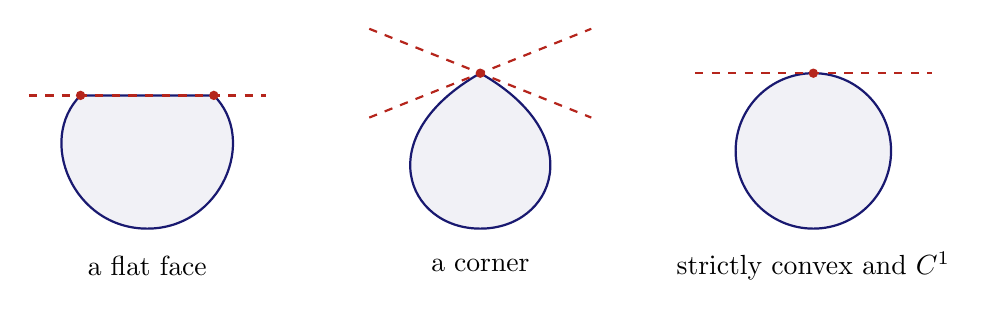
\begin{tikzpicture}[scale=0.94,line width=0.8pt,
  body/.style={draw=MidnightBlue,fill=MidnightBlue!6},
  support/.style={draw=BrickRed,dashed}]
 \begin{scope}[xshift=-4.5cm]
  \path[body] (-0.9,0.7)--(0.9,0.7)
   .. controls (1.5,0.1) and (1,-1.1) .. (0,-1.1)
   .. controls (-1,-1.1) and (-1.5,0.1) .. (-0.9,0.7);
  \draw[support] (-1.6,0.7)--(1.6,0.7);
  \fill[BrickRed] (-0.9,0.7) circle (1.8pt) (0.9,0.7) circle (1.8pt);
  \node at (0,-1.6) {a flat face};
 \end{scope}
 \begin{scope}
  \path[body] (0,1) .. controls (1.5,0.15) and (1,-1.1) .. (0,-1.1)
   .. controls (-1,-1.1) and (-1.5,0.15) .. (0,1);
  \draw[support] (-1.5,1.6)--(1.5,0.4);
  \draw[support] (-1.5,0.4)--(1.5,1.6);
  \fill[BrickRed] (0,1) circle (1.8pt);
  \node at (0,-1.6) {a corner};
 \end{scope}
 \begin{scope}[xshift=4.5cm]
  \path[body] (0,-0.05) circle (1.05);
  \draw[support] (-1.6,1)--(1.6,1);
  \fill[BrickRed] (0,1) circle (1.8pt);
  \node at (0,-1.6) {strictly convex and $C^1$};
 \end{scope}
\end{tikzpicture}
\caption{The two obstructions to regularity. These are schematic convex
bodies; the circle is not a proposed formula for the limit shape.}
\label{fig:geometry}
\end{figure}

\subsection{History and significance}

First-passage percolation was introduced by Hammersley and Welsh
\cite{HW1965}. The asymptotic-shape theory developed through the work of
Richardson \cite{Richardson1973} and Cox and Durrett \cite{CD1981},
alongside Kingman's ergodic theory of subadditive processes
\cite{Kingman1968}.
Although the shape theorem gives a convex deterministic body, its fine
geometry is much harder to determine; see the survey of Auffinger,
Damron, and Hanson \cite{ADH2017}. Theorem~\ref{thm:exponential-shape}
resolves positively the strict-convexity and differentiability
conjectures for the planar exponential model.

There are important partial results for both questions. Lalley
\cite{Lalley2003} gave sufficient conditions for strict convexity in
the standard lattice model, involving asymptotic straightness and
mean-zero scaling limits. In Richardson's site growth model, Durrett
and Liggett \cite{DurrettLiggett1981} established a flat edge for
parameters sufficiently close to one and identified its onset with the
threshold of a related contact process. For planar edge first-passage
percolation with support minimum normalized to one and an atom of mass $p$
there, Marchand \cite[Theorem~1.3]{Marchand2002} determined the exact
flat segment on the first-quadrant unit $\ell^1$ boundary when
$p>\vec p_c$, where $\vec p_c$ is the oriented-percolation threshold,
and a single diagonal contact point when $p=\vec p_c$. For finite-mean
laws in this class with $\vec p_c\le p<1$, Auffinger and Damron
\cite[Theorem~2.1]{AD13} proved differentiability at the endpoints,
including the critical contact point. These last two results concern
an atom at a positive minimum; exponential edge weights are nonatomic
and have essential infimum zero.

The connection between shape geometry and geodesics was developed by
Newman and Licea--Newman \cite{Newman1995,LiceaNewman1996}. Curvature
hypotheses and fixed-direction uniqueness play distinct roles in those
results. Damron and Hanson \cite{DH2017}
proved convergence and coalescence toward a specified supporting sector
under differentiability assumptions. Our two regularity conclusions
make that sector a single direction. Section~\ref{sec:consequences}
states the resulting geodesic and Busemann conclusions with the
direction fixed before the probability-one event is chosen. The
midpoint question of Benjamini, Kalai, and Schramm \cite{BKS2003}
is already answered qualitatively without shape regularity by Ahlberg
and Hoffman \cite{AH2019}. We explain its relation to the directional
results. For all Gamma laws, differentiability supplies infinitely
many extreme points, making the quantitative midpoint estimate of
Dembin, Elboim, and Peled \cite{DEP2024} applicable as well.

\subsection{Proof strategy}

\paragraph{Excluding a corner.}
Suppose two distinct extreme supporting functionals $f_-,f_+$ touch
the norm in a direction $u$, and let $f=(f_-+f_+)/2$. Their gap gives
a linear penalty for transverse motion. Part~\ref{part:differentiability}
turns this penalty into a positive excess over $f$ for every sufficiently
long simple path, contradicting the shape theorem along $u$.

First, a crossing confined to a long narrow strip is unlikely to save
a fixed multiple of the strip width over either extreme support.
Otherwise independent parallel trials, connected using one-sided
first-order contact with the norm, would yield macroscopic travel
below that support. Second, a finite-region change of measure produces
characteristic lengths $L$ for widths $s$, with $L/s\to\infty$ and
$L\le s^3$. Nested grids then extend the crossing estimate to arbitrary
endpoints, with a summable cost. Third, every cheap path chunk contains
a witness for a rare decreasing event. The van den Berg--Kesten
inequality \cite{BK85}, applied to disjoint edge witnesses, handles
repeated visits to the same coarse box and yields a bound for all
long simple paths at once. The counting builds on Kesten's rectangle
itineraries and crossing-multiplicity estimates
\cite[Section~3]{Kesten1980}; here the local witnesses certify negative
excess relative to a supporting functional.

The Gamma extension is built into this proof. Its distributional inputs
are exponential tails for short coordinate paths, a continuous quantile
representation for the witness inequality, and an exact likelihood
calculation: scaling one Gamma weight by $1-\delta$ gives likelihood
second moment $(1-\delta^2)^{-\kappa}$. Scaling $O(ns)$ weights with
$\delta$ of order $s/n$ has bounded second moment when $n=s^3$.
No differentiability or curvature estimate for $\mu$ enters these inputs.

\paragraph{Excluding a flat face.}
Under a hypothetical flat face, the stationary cocycle construction of
Damron and Hanson \cite{DH2014} supplies an additive random function
$B(x,y)$, with mean the supporting functional and with
$|B(x,y)|\le T(x,y)$. Thus a path from $x$ to $y$ has nonnegative
defect $\tau(P)-B(x,y)$. Part~\ref{part:strict} considers local random
paths, called roads, tracking two directions near the ends of the face.
At lattice scale $n$, let $b(n)$ be the infimum of a common upper bound
for their mean defect per period. A local perturbation gives
$b(n)\ge c_0>0$. The main construction gives a fixed integer $D$ and
$\rho<1$ such that
\[
 b(Dn)\le\rho b(n).
\]
Iteration contradicts the positive lower bound.

A finite-cell projection constructs local endpoint potentials
approximating increments of the generally nonlocal cocycle; interpolation
controls every possible attachment in a bounded road interval
(Section~\ref{found:sec-gauges}). A physical routing argument bounds the
savings obtainable from a selected collection of local shortcuts
(Proposition~\ref{access:collection}). An area-preserving deformation
then controls those savings along paths concentrated near an extreme
direction (Lemma~\ref{probability:thin-tails}). Passage-time concentration
and mean approximation estimates of Damron--Hanson--Sosoe \cite{DHS2014}
and Damron--Kubota \cite{DK2016} supply the quantitative metric input.

These estimates let a long geodesic toward an extreme endpoint supply
many crossings between neighboring walls while controlling the discarded
pieces. The extraction gives a small upper bound for the mean clipped
cost of a local crossing. Comparing this crossing with the current road, including the
short wall connections, transfers the clipped bound to a primary
candidate. To control the remaining large positive costs, a local rule
groups their flags into short clusters and traverses an independently
built spare road across each accepted cluster, with forward connections
at both ends (Lemma~\ref{improvement:replacement}). A matched cap controls
the frequency of flags, while separation and first-moment estimates
control the added cost. This reduces the full expected excess per road
period. A fixed rescaling restores the required tracking and locality,
so the improved paths belong to the class defining $b(n)$.

The two arguments use different endpoint corrections. In
Part~\ref{part:differentiability}, the deterministic defect
$\tau(P)-f(\Delta P)$ can be negative. In Part~\ref{part:strict}, the
cocycle defect is nonnegative on every forward subpath. Each part
introduces its own local coordinates and parameters.

\clearpage
\part{Differentiability for Gamma weights}
\label{part:differentiability}
\section{Shape estimates and supporting functionals}
\label{df:sec:setup}

Fix $\kappa,\lambda>0$ throughout this part and write
$\mu=\mu_{\kappa,\lambda}$. All constants and scale thresholds may
depend on this fixed law. We shall compare path costs with the two
extreme supporting functionals at a prescribed direction. The crossing
estimates use only their one-sided contact with $\mu$; the assumption
that they differ enters the final contradiction.

\subsection{Uniform shape and local sums}

We first record the precise form of the standard shape theorem that
will be used. It holds for the fixed Gamma law:
\begin{equation}\label{df:eq:uniform-shape}
 \sup_{z\in\Z^2:\,|z|\ge R}
 \frac{|T(0,z)-\mu(z)|}{|z|}\longrightarrow0
 \qquad\text{almost surely as }R\to\infty.
\end{equation}
This is the shape theorem of
\cite[Theorem~A.1 and Equation~(A.3)]{KRS23}, at weight shift zero.
The Gamma law has essential infimum zero and no atom there. For
four independent copies of an edge weight,
\[
 \E\!\left[\min\{\tau_1,\tau_2,\tau_3,\tau_4\}^2\right]
 \le \E[\tau_1^2]
 =\frac{\kappa(\kappa+1)}{\lambda^2}<\infty.
\]
These facts verify the cited hypotheses. The source uses $\ell^1$
distance, which gives \eqref{df:eq:uniform-shape} by equivalence of
norms. There are deterministic constants $0<\alpha\le\beta<\infty$ such that
\begin{equation}\label{df:eq:norm-bounds}
 \alpha|z|\le\mu(z)\le\beta|z|\qquad(z\in\R^2).
\end{equation}
An event expressed relative to a deterministic lattice origin has the
same probability at every translate. This observation will allow us to
use shape estimates in probability at origins that vary with the
scale. Equation~\eqref{df:eq:uniform-shape} itself is an almost-sure
statement simultaneously over all endpoints from the fixed origin.

Almost surely every edge weight is finite and positive, since there
are only countably many edges. In particular, loop erasure does not
increase cost. A path constrained to a set will mean a path all of
whose vertices belong to that set; such path-existence events use
only its internal edges. Concatenated paths may retrace edges, with
each traversal contributing to the cost.

The following bound controls the vertical attachments used below.

\begin{lemma}[Gamma exponential moments]\label{df:ga:moment}
For $\tau\sim\operatorname{Gamma}(\kappa,\lambda)$ and $\theta<\lambda$,
\[
 \E e^{\theta\tau}
 =\left(\frac{\lambda}{\lambda-\theta}\right)^\kappa.
\]
If $V$ is the sum over a deterministic set of $M$ distinct edges and
$M\le A v$, where $A,v>0$, then
\begin{equation}\label{df:eq:gamma-sum-tail}
 \PP\left(V>\frac{2A\kappa}{\lambda}v\right)
 \le \exp\{-A\kappa(1-\log 2)v\}.
\end{equation}
\end{lemma}

\begin{proof}
Integrating the Gamma density with the substitution
$y=(\lambda-\theta)t$ gives the moment identity. At
$\theta=\lambda/2$ it reads $\E e^{\lambda\tau/2}=2^\kappa$.
Independence and exponential Markov inequality give
\[
 \PP\left(V>\frac{2A\kappa}{\lambda}v\right)
 \le e^{-A\kappa v}2^{\kappa M}
 \le e^{-A\kappa(1-\log 2)v}.
\]
\end{proof}

\subsection{The two extreme supports}

Signed coordinate permutations preserve the law and hence $\mu$.
Together with positive homogeneity, these symmetries reduce the proof
to directions
\[
 u=(1,b),\qquad -1\le b\le1.
\]
Fix such a deterministic direction for the rest of the argument, and
write
\[
 x(z)=z_1,\qquad r(z)=z_2-bz_1,
 \qquad m_0=\mu(u)>0.
\]
The function $t\mapsto\mu(u+te_2)$ is convex and Lipschitz. Let
\[
 a_- = \lim_{t\uparrow0}\frac{\mu(u+te_2)-m_0}{t},
 \qquad
 a_+ = \lim_{t\downarrow0}\frac{\mu(u+te_2)-m_0}{t}.
\]
These finite limits satisfy $a_-\le a_+$. Define
\begin{equation}\label{df:eq:support-definitions}
 \begin{split}
 f_\pm(z)&=m_0x(z)+a_\pm r(z),\\
 a&=\frac{a_-+a_+}{2},\qquad
 c=\frac{a_+-a_-}{2},\qquad
 f(z)=m_0x(z)+ar(z).
 \end{split}
\end{equation}

\begin{lemma}[One-sided contact]\label{df:prelim:supports}
The linear functionals $f_-$, $f_+$, and $f$ are bounded above by
$\mu$ on $\R^2$ and equal $\mu$ at $u$. For
$\sigma\in\{-,+\}$, with the corresponding numerical sign when
multiplied by a scalar,
\begin{equation}\label{df:eq:support-contact}
 \mu(u+te_2)-f_\sigma(u+te_2)=o(|t|)
 \qquad(t\to0,\ \sigma t>0).
\end{equation}
\end{lemma}

\begin{proof}
Each of $a_-$ and $a_+$ is a subgradient at zero of the convex
function $t\mapsto\mu(u+te_2)$. If $x(z)>0$, write
$z=x(z)(u+r(z)x(z)^{-1}e_2)$ and use positive homogeneity to get
$f_\sigma(z)\le\mu(z)$. If this inequality failed at any other
point $z$, then a sufficiently small positive convex combination of
$z$ with $u$ would still violate it, by convexity, and would have
positive first coordinate. This is impossible. The average $f$ is
also bounded above by $\mu$. Equation~\eqref{df:eq:support-contact}
is the respective one-sided derivative expansion.
\end{proof}

The \emph{defect} of a path is its cost minus the value of a supporting
functional on its displacement. We shall use
\begin{equation}\label{df:eq:defects}
 H(P)=\tau(P)-f(\Delta P),\qquad
 H_\sigma(P)=\tau(P)-f_\sigma(\Delta P).
\end{equation}
They are additive under concatenation, and
\begin{equation}\label{df:eq:minimum-defect}
 \min\{H_+(P),H_-(P)\}=H(P)-c|r(\Delta P)|.
\end{equation}
The crossing and endpoint estimates will hold for both signs whether
or not $c$ is positive. In Section~\ref{df:sec:witnesses}, the gap
assumption $c>0$ and \eqref{df:eq:minimum-defect} will make transverse
exits expensive relative to the average support $f$.

\section{Localized crossings}\label{df:sec:crossings}

The main estimate in this section is Lemma~\ref{df:cr:rare-fast}: a crossing
confined to a strip of width of order $s$ is unlikely to have defect below
$-\varepsilon s$ when its length is much larger than $s$. The proof amplifies
any positive probability of such a crossing into an infinite concatenation
whose defect decreases linearly, contradicting the shape theorem.

We prepare three ingredients for this construction. The shape theorem first
gives short paths confined near their joining segments. A finite net then
makes this assertion simultaneous over all endpoints in two intervals.
Finally, an oriented-percolation argument joins sufficiently likely local
tests even when nearby tests overlap. Throughout the section, distances are
Euclidean unless indicated otherwise. A path constrained to a region has
all its vertices there, so its existence and cost are tested using only
edges with both endpoints in that region.

\begin{lemma}[Localized travel]\label{df:cr:local-travel}
Fix $D,\eta,\delta>0$. Uniformly over deterministic vertices $p,q\in\Z^2$
with $|q-p|\le Ds$, the probability tends to one as $s\to\infty$
that there is a path from $p$ to $q$ with cost at most
\[
  \mu(q-p)+\eta s
\]
whose vertices are within distance $\delta s$ of the segment $[p,q]$.
\end{lemma}

\begin{proof}
\emph{Uniform shape estimates.}
Use the constants $\alpha,\beta$ from \eqref{df:eq:norm-bounds}.
Equation~\eqref{df:eq:uniform-shape} implies, for each fixed $C>0$,
\begin{equation}\label{df:eq:cr-uniform-shape}
 \frac1s\max_{\substack{z\in\Z^2\\|z|\le Cs}}
       \abs{T(0,z)-\mu(z)}\longrightarrow0
 \qquad\text{almost surely}.
\end{equation}
Indeed, outside any sufficiently large fixed ball the error is bounded by an
arbitrarily small multiple of $|z|$, while the finitely many passage
times inside that ball contribute $o(s)$. The same shape theorem gives
\begin{equation}\label{df:eq:cr-escape}
 \PP\left(
   \inf_{\substack{z\in\Z^2\\|z|\ge\delta s/3}}
       T(0,z)\ge\alpha\delta s/6
       \right)\longrightarrow1.
\end{equation}
Translation invariance gives the same probability bounds at every
deterministic lattice origin. This uniformity will allow the origins to
depend on the endpoints and on $s$.

\emph{Short pieces cannot escape.}
Choose a fixed integer $B$ so large that $\beta D/B<\alpha\delta/24$.
Round the $B+1$ equally spaced points of $[p,q]$ to vertices
$p_0=p,p_1,\ldots,p_B=q$. Uniformly in the endpoints,
\[
 \mu(p_{j+1}-p_j)=\frac{\mu(q-p)}{B}+O(1).
\]
Apply \eqref{df:eq:cr-uniform-shape} and \eqref{df:eq:cr-escape} at these
finitely many deterministic vertices. With probability tending to one,
uniformly in $p,q$, every short passage time is at most
\[
 \frac{\mu(q-p)}B+
       \min\left\{\frac{\eta}{2B},\frac{\alpha\delta}{24}\right\}s,
\]
and escape from the ball of radius $\delta s/3$ about its starting vertex
costs at least $\alpha\delta s/6$. For each $j=0,\ldots,B-1$, choose a path
from $p_j$ to $p_{j+1}$ with cost at most $T(p_j,p_{j+1})+1$.
For all sufficiently large $s$, each chosen path has cost strictly below
the corresponding escape bound. Nonnegativity of the weights forces it
to stay inside the ball about $p_j$: its initial portion up to a vertex
outside would already cost at least the escape bound.

\emph{Concatenation.}
Concatenating the $B$ paths gives total cost
at most $\mu(q-p)+\eta s/2+B\le\mu(q-p)+\eta s$. Each ball is centered
within bounded distance of the original segment, so it lies in its
$\delta s$-neighborhood for large $s$. All probability bounds used above
are uniform in the deterministic vertices, proving the stated uniformity.
\end{proof}

The next form permits the endpoints to be selected after the environment
is observed. The intervals themselves remain deterministic, and the
assertion holds for every endpoint pair on one event of high probability.

\begin{lemma}[Travel between intervals]\label{df:cr:interval-travel}
Fix $D,\eta,\delta>0$. Let $I_1,I_2$ be deterministic vertical intervals
on lattice columns, and suppose that the diameter of $I_1\cup I_2$ is at
most $Ds$. Uniformly over their locations, with probability tending to
one as $s\to\infty$, every pair
$p\in I_1\cap\Z^2$, $q\in I_2\cap\Z^2$ can be joined by a path of
cost at most $\mu(q-p)+\eta s$ within distance $\delta s$ of $[p,q]$.
\end{lemma}

\begin{proof}
The assertion is vacuous if either interval contains no vertex.

\emph{Finite nets and vertical attachments.}
Let $\beta$ be the upper norm bound in \eqref{df:eq:norm-bounds}, and
choose a fixed $\gamma>0$ so small that
\[
 \left(\frac{4\kappa}{\lambda}+2\beta\right)\gamma\le\eta/2,
 \qquad \gamma\le\delta/2.
\]
In each interval, choose a net of lattice vertices containing its extreme
lattice vertices and having consecutive gaps at most
$\lfloor\gamma s\rfloor$. For all large $s$, each net needs at most
$2D/\gamma+2$ vertices. Assign every interval vertex to a net vertex at
vertical distance at most $\gamma s$, using only edges of its intervening gap.

For any such gap, the total weight $V$ is a sum of at most
$\lfloor\gamma s\rfloor$ independent edge weights.
Lemma~\ref{df:ga:moment}, with $A=\gamma$ and $v=s$, gives
\[
 \PP\left(V>\frac{2\kappa}{\lambda}\gamma s\right)
 \le e^{-\kappa(1-\log2)\gamma s}.
\]
There are only boundedly many gaps. Thus, with probability tending to
one, all vertical connections from interval vertices to their chosen
net vertices cost at most $2\kappa\gamma s/\lambda$.

\emph{Connections between net vertices.}
Apply Lemma~\ref{df:cr:local-travel}, with errors $\eta/2$ and $\delta/2$,
to every pair of net vertices. Its uniformity and the bounded number
of pairs give these connections simultaneously.

\emph{All endpoint pairs on the same event.}
On the intersection of these high-probability events, take arbitrary
$p\in I_1\cap\Z^2$ and $q\in I_2\cap\Z^2$. Concatenate their vertical
attachments with the path between the assigned net vertices
$\widehat p,\widehat q$. The resulting cost is at most
\[
 \begin{split}
 \mu(\widehat q-\widehat p)+\eta s/2
       +\frac{4\kappa}{\lambda}\gamma s
 &\le \mu(q-p)+\eta s/2
       +\left(\frac{4\kappa}{\lambda}+2\beta\right)\gamma s.
 \end{split}
\]
The segments $[p,q]$ and $[\widehat p,\widehat q]$ have Hausdorff distance
at most $\gamma s$. The choice of $\gamma$ therefore gives both the cost
bound and the required localization, including the vertical attachments.
The same event works for every $p,q$, and its probability bound is uniform
in the deterministic locations of the intervals.
\end{proof}

We will place local crossing and connection tests on an auxiliary copy of
$\Z^2$. The following elementary lemma needs only a uniform bound on their
failure probabilities and independence at sufficiently separated sites.

\begin{lemma}[High-density oriented paths]\label{df:cr:oriented-paths}
For every integer $k_0\ge0$ there is $\zeta=\zeta(k_0)>0$ with the
following property. Let $(G_v)_{v\in\Z^2}$ be events such that any finite
family indexed by sites at pairwise sup distance greater than $k_0$ is
independent. If $\PP(G_v^c)\le\zeta$ for every $v$, then with positive
probability there is an infinite path starting at $0$, using steps
$(1,0)$ and $(0,1)$, all of whose sites satisfy $G_v$.
\end{lemma}

\begin{proof}
\emph{A finite reachable set if there is no infinite path.}
Call a site good when $G_v$ occurs. Let $S$ consist of the endpoints of
finite oriented paths from $0$ for which every site except possibly the
last is good. In particular $0\in S$. If $S$ were infinite, the finitely
branching tree of these paths would have an infinite branch; every site
on that branch would be good. Hence, on the event of no infinite good
path, $S$ is finite.

\emph{A surrounding contour forces bad sites.}
For such a finite $S$, orient the boundaries of the unit squares centered
at its sites counterclockwise and cancel shared sides. The remaining
edges form a balanced directed graph and hence decompose into closed
directed trails, with no edge repeated in a trail. Repeated vertices are
allowed, so corner contacts cause no difficulty. Every edge has an
$S$-square on its left and a complementary square on its right.
Winding number is additive under cancellation and decomposition. Its
total about $0$ is one, contributed by the square centered at $0$;
therefore some trail has nonzero winding.

Let $m$ be the length of this trail. Closedness implies that exactly
$m/2$ of its steps are upward or leftward. For these steps, the site on
the right is respectively an east or north neighbor of the site on the
left. The left-hand site must be bad: if it were good, extending a path
that reaches it would put this neighbor in $S$ as well.

\emph{Independent bad sites along a fixed contour.}
A site borders at most four edges of the trail, so at least $m/8$
distinct sites are forced to be bad. For any fixed candidate trail these
sites are deterministic. Greedy selection in a fixed order gives at least
\[
 \frac{m}{8(2k_0+1)^2}
\]
of them at pairwise sup distance greater than $k_0$: each selected site
removes at most $(2k_0+1)^2$ candidates. Their tests are independent, so
the probability of all the badness conditions forced by this particular
trail is at most $\zeta^{m/[8(2k_0+1)^2]}$.

\emph{Summing over contours.}
Nonzero winding forces $0$ into the coordinate bounding box of the
trail. A length-$m$ trail has coordinate spans at most $m$, so it lies
in a square of side $O(m)$ about $0$. Choosing its starting vertex and
then its step sequence bounds the number of candidates by
$C(m+1)^2 4^m$. Consequently the probability of no infinite good path
is at most
\[
 \sum_{m\ge4} C(m+1)^2
       \left(4\zeta^{1/[8(2k_0+1)^2]}\right)^m.
\]
This is less than one when $\zeta$ is sufficiently small. The argument
uses no stationarity assumption on the tests.
\end{proof}

We now combine these ingredients. The relevant defect is measured against
one of the extremal supports $f_\sigma$. Its one-sided contact with $\mu$
allows successive crossings to be connected with defect as small a multiple
of $s$ as needed, by drifting consistently to the corresponding side of
the direction $u$.

\begin{lemma}[Rare fast localized crossings]\label{df:cr:rare-fast}
Fix $A,R,\varepsilon>0$ and $\sigma\in\{-,+\}$. As $s\to\infty$ and
$n/s\to\infty$, with $s$ real and $n$ a positive integer,
\begin{equation}\label{df:eq:cr-rare-fast}
 \PP\left(
 \begin{array}{l}
 \text{there is a path $P$ from $x=0$ to $x=n$ with}
       \ H_\sigma(P)<-\varepsilon s,\\
 \text{all of whose vertices satisfy }
       -An\le x\le(1+A)n,\quad |r|\le Rs
 \end{array}\right)\longrightarrow0.
\end{equation}
The same assertion holds, with the same probability, for every exact
lattice translate of the event.
\end{lemma}

\begin{proof}
Suppose that the probability in \eqref{df:eq:cr-rare-fast} is at least
$p_0>0$ along a sequence satisfying the stated limits. At each auxiliary
site we will try several disjoint translates of this crossing event and
require connections to both forward neighbors. Enough trials make a
successful crossing likely; the one-sided contact estimate makes the
connections likely without spending the whole crossing deficit.

\emph{1. Parameters and site geometry.}
The dependence radius must be fixed before we choose how many trials to
make. Set
\[
 k_0=\left\lceil4(A+3)+8\right\rceil+1
\]
and let $\zeta$ be supplied by Lemma~\ref{df:cr:oriented-paths}. Choose a
fixed integer $M$ so large that $(1-p_0)^M<\zeta/2$. For each member of
the sequence put
\[
 S_0=100M(R+1)\lceil s\rceil,
 \qquad d=\lceil D_0s\rceil,
\]
where the fixed constant $D_0$ will be chosen below, after $M$.

Identify the signs $+$ and $-$ with $1$ and $-1$ when they multiply
coordinates. For a test site $v=(v_1,v_2)\in\Z^2$, write
\[
 i=v_1+v_2,
 \qquad X_i=i(n+d),
 \qquad Y_v=\sigma(i+v_2)S_0.
\]
An oriented step sends $i$ to $i+1$ and changes $Y_v$ by $\sigma S_0$
or $2\sigma S_0$. Thus every step advances to the next longitudinal
block and moves transversely to the same prescribed side.

\emph{2. Independent crossing trials within a site.}
At site $v$, make $M$ trials using exact lattice translates of the event
in \eqref{df:eq:cr-rare-fast}, all with initial column $X_i$, and with their
strips disjoint and contained in $|r-Y_v|\le S_0/4$. Here is an explicit
choice, which also accounts for lattice phases. Put
\[
 h_j=(2j-M-1)\,3(R+1)\lceil s\rceil,
 \qquad
 t_{v,j}=\left(X_i,
    \left\lfloor bX_i+Y_v+h_j+\tfrac12\right\rfloor\right),
 \quad 1\le j\le M.
\]
The translated strip has center $r(t_{v,j})$, within $1/2$ of
$Y_v+h_j$. For $s\ge1$, consecutive centers are separated by more than
$2Rs$, and every strip of half-width $Rs$ lies inside the designated
$S_0/4$ window. Thus the trials use disjoint internal edge sets.
Translation leaves both displacement and its supporting functional
unchanged, so each trial has probability at least $p_0$, exactly as in
the original event. Their probability of all failing is at most
$(1-p_0)^M$.

\emph{3. Connection tests for every endpoint pair.}
For each of the two forward neighbors $v'$ of $v$, impose an additional
test. Every vertex on
\[
 x=X_i+n,\quad |r-Y_v|\le S_0/4
\]
must be connectible to every vertex on
\[
 x=X_{i+1},\quad |r-Y_{v'}|\le S_0/4
\]
by a path of cost at most $f_\sigma$ of its displacement plus
$\varepsilon s/2$, lying in
\begin{equation}\label{df:eq:cr-connector-region}
 X_i+n-s\le x\le X_{i+1}+s,
 \qquad |r-Y_v|\le4S_0.
\end{equation}
These are existence tests using only the internal edges of this region.
Requiring every endpoint pair will permit the successful trials to be
chosen later, after the environment has been observed.

\emph{4. Choosing the connector length.}
We next choose $D_0$ and verify that both connection tests pass with
probability tending to one uniformly in $v$. A connector displacement
$z$ satisfies
\[
 x(z)=d,
 \qquad S_0/2\le\sigma r(z)\le5S_0/2\le3S_0.
\]
Set $C_0=200M(R+1)$, so that $S_0/s\le C_0$ for $s\ge1$.
The one-sided expansion \eqref{df:eq:support-contact} supplies $h_0>0$
such that
\[
 0\le\mu(u+h e_2)-f_\sigma(u+h e_2)
       \le\frac{\varepsilon}{12C_0}|h|
 \quad\text{if }0<\sigma h\le h_0.
\]
Choose $D_0\ge1$ with $3C_0/D_0\le h_0$. For every possible connector,
$h=r(z)/d$ is on the required side and has absolute value at most $h_0$.
Homogeneity therefore gives
\[
 \mu(z)-f_\sigma(z)
   \le\frac{\varepsilon}{12C_0}|r(z)|\le\varepsilon s/4.
\]
This leaves another $\varepsilon s/4$ for the travel error.

The two endpoint intervals have union diameter at most $Ds$ for a fixed
$D$ depending only on $M,R,D_0$. Their joining segments have longitudinal
coordinates between the two endpoint columns and satisfy
$|r-Y_v|\le9S_0/4$. Since $|b|\le1$, moving Euclidean distance
$\delta s$ changes $x$ by at most $\delta s$ and $r$ by at most
$\sqrt2\delta s$. Thus a tube with any fixed $0<\delta\le1/2$ fits
inside \eqref{df:eq:cr-connector-region}. Lemma~\ref{df:cr:interval-travel},
with cost error $\varepsilon s/4$, proves the required connection assertions
simultaneously for all endpoint pairs. Its probability estimate is
uniform in the intervals' locations, including their lattice phases.

\emph{5. A dependence radius independent of the later choices.}
Call $v$ good when at least one of its trials succeeds and both connection
tests pass. Its bad probability is at most
$(1-p_0)^M+o(1)$, uniformly in $v$. We verify that the initially chosen
$k_0$ is a dependence radius. Take a sufficiently large member of the
sequence that $n\ge d+s$. The entire test at $v$ is supported on internal
edges in
\[
 |x-X_i|\le(A+3)n,
 \qquad |r-Y_v|\le4S_0.
\]
To compare two sites, use the integer coordinates $i=v_1+v_2$ and
$j=i+v_2$. If their support regions share a vertex, the longitudinal
and transverse bounds give, respectively,
\[
 |\Delta i|\le2(A+3),
 \qquad |\Delta j|\le8,
\]
where $\Delta$ denotes the difference between the two sites.
Since $v_2=j-i$ and $v_1=2i-j$, this implies
\[
 |\Delta v_2|\le2(A+3)+8,
 \qquad |\Delta v_1|\le4(A+3)+8<k_0.
\]
Tests at sites at pairwise sup distance greater than $k_0$ therefore use
pairwise disjoint edge sets and are jointly independent. In particular,
the dependence radius does not increase when $M$ or $D_0$ is chosen.
The order of choices was consequently legitimate: $k_0$ and $\zeta$
first, then $M$, then $D_0$, and finally a sufficiently large member of
the sequence. For that member the bad probability is at most $\zeta$.

\emph{6. Concatenation at one fixed scale.}
By Lemma~\ref{df:cr:oriented-paths}, with positive probability there is an
infinite oriented path of good sites starting at $0$. Fix this one scale
$s,n,d,S_0$ and a configuration with such a path. At each visited site
choose a successful trial and join it to the next by a tested connector.
Prepend a vertical path from the lattice origin to the initial trial's
starting vertex; its defect $H_\sigma$ is a finite random quantity $C$.
If $z_t$ is the endpoint of the trial at the $t$th site, with the initial
site numbered $0$, additivity gives a path from $0$ to $z_t$ of defect
at most
\begin{equation}\label{df:eq:cr-linear-deficit}
 C-(t+1)\varepsilon s+t\varepsilon s/2.
\end{equation}
The trials and connectors need not be disjoint: costs are counted with
edge multiplicities, so their concatenation still bounds passage time
from above.

\emph{7. The shape-theorem contradiction.}
At that site, $i=t$ and $0\le v_2\le t$. Hence
\[
 x(z_t)=t(n+d)+n,
 \qquad |r(z_t)|\le2tS_0+S_0/4.
\]
Thus $|z_t|\to\infty$ and $|z_t|\le C'(t+1)$ for a deterministic
constant $C'$ at this fixed scale. The limit here is $t\to\infty$;
the parameters $s,n,d,S_0$ remain fixed. On the probability-one event
of the origin shape theorem, its uniform outside-ball estimate applies
also to these adaptively chosen endpoints and yields
\[
 T(0,z_t)\ge\mu(z_t)-o(t)\ge f_\sigma(z_t)-o(t),
\]
where the supporting inequality is from Lemma~\ref{df:prelim:supports}.
This contradicts \eqref{df:eq:cr-linear-deficit}, whose negative part grows
at least as $t\varepsilon s/2$. The infinite-path event consequently has
probability zero, contradicting its construction. No sequence with
crossing probability bounded below by $p_0$ exists, proving the asserted
joint limit. Exact lattice-translation invariance proves the last assertion.
\end{proof}

\section{Characteristic lengths}\label{df:sec:scales}

The rare-fast estimate concerns crossings with a negative defect.
We next identify a length at which crossings are rare even with a
positive allowance of order the strip width. A finite-region change
of measure supplies an upper bound on that length. Its definition
then guarantees enough shorter crossings to construct the endpoint
extensions in the next section.

Small multiplicative changes of many independent weights, with a
controlled quadratic probability cost, also appear in fluctuation
arguments; see Chatterjee \cite{Chatterjee2019}. Here the exact Gamma
likelihood calculation is valid for every positive shape parameter.

\subsection{A first crossing threshold}

Set
\[
 K=100\bigl(1+\abs{a_-}+\abs{a_+}\bigr).
\]
For real $s\geq1$ and integer $n\geq1$, let $E(s,n)$ be the event that
there is a finite path $P$ from the column $x=0$ to the column $x=n$,
with every vertex in
\[
 \{-n\leq x\leq2n,\ \abs{r}\leq8s\},
\]
and with
\[
 \tau(P)<m_0n+Ks.
\]
Endpoints on the two columns are unrestricted within this region. As
throughout, the event tests only the internal edges of the indicated
region. The notation $E(s,n)$ will also be used with an explicitly
specified lattice translation.

\begin{lemma}[Rarity at cubic length]\label{df:gr:tilt}
For $s=2^k$ and $k\to\infty$,
\[
 \PP\bigl(E(s,s^3)\bigr)\longrightarrow0.
\]
\end{lemma}
\begin{proof}
\emph{Turning an allowed crossing into a fast crossing.}
Put $n=s^3$. Choose a fixed $\eta>0$ such that
\[
 \eta m_0>K+16\abs{a_+}+1,
\]
and set $\delta=\eta s/n$ and $\alpha=1-\delta$. Take $s$ sufficiently
large that $0<\delta\le1/2$. Multiply every internal edge weight of the
region defining $E(s,n)$ by $\alpha$, leaving the other weights
unchanged. If $P$ witnesses $E(s,n)$ before this operation, its
transverse displacement obeys $\abs{r(\Delta P)}\le16s$, and in the
modified environment
\[
 \begin{split}
 H_+(P)
 &<\alpha(m_0n+Ks)-m_0n-a_+r(\Delta P)\\
 &\le \bigl(K-\eta m_0+16\abs{a_+}\bigr)s
          -\eta K\frac{s^2}{n}<-s.
 \end{split}
\]
This computation includes every traversal if $P$ repeats an edge.
Let $F(s,n)$ be the crossing event $H_+(P)<-s$ in the same region, and
let $Q$ be the law of the modified environment. The deterministic
implication gives
\begin{equation}\label{df:eq:gr-tilt-implication}
 \PP(E(s,n))\le Q(F(s,n)).
\end{equation}

\emph{The cost of the change of measure.}
Under $Q$, a modified edge has distribution
$\operatorname{Gamma}(\kappa,\lambda/\alpha)$. On $t>0$ its likelihood
ratio with respect to the original edge law is
\[
 L_\delta(t)
 =\frac{p_{\kappa,\lambda/\alpha}(t)}{p_{\kappa,\lambda}(t)}
 =\alpha^{-\kappa}
    \exp\{-\lambda(\alpha^{-1}-1)t\}.
\]
Both densities are positive on $(0,\infty)$, including when
$0<\kappa<1$. Direct integration gives
\[
 \begin{split}
 \E[L_\delta(\tau_e)^2]
 &=\alpha^{-2\kappa}\frac{\lambda^\kappa}{\Gamma(\kappa)}
   \int_0^\infty t^{\kappa-1}
     e^{-\lambda(2/\alpha-1)t}\,\mathrm d t\\
 &=\alpha^{-2\kappa}(2/\alpha-1)^{-\kappa}
   =\bigl(\alpha(2-\alpha)\bigr)^{-\kappa}
   =(1-\delta^2)^{-\kappa}.
 \end{split}
\]
The region has at most $(3n+1)(16s+2)$ vertices and at most twice that
many internal unoriented edges. Thus the number $M$ of modified
coordinates is at most $144ns$. The likelihood ratio is a product
over these distinct coordinates, regardless of path multiplicity.
By independence,
\[
 \begin{split}
 \E\left[\left(\frac{\mathrm d Q}{\mathrm d\PP}\right)^2\right]
 &=(1-\delta^2)^{-\kappa M}
 \le \exp(2\kappa M\delta^2)\\
 &\le \exp\left(288\kappa\eta^2\frac{s^3}{n}\right)
 =\exp(288\kappa\eta^2).
 \end{split}
\]
\emph{Transfer back to the original law.}
Lemma~\ref{df:cr:rare-fast}, applied under the original law with $A=1$,
$R=8$, and $\varepsilon=1$, gives $\PP(F(s,n))\to0$ because $n/s=s^2\to\infty$.
Cauchy--Schwarz therefore gives
\[
 \PP(E(s,n))\le Q(F(s,n))
 \le e^{144\kappa\eta^2}\PP(F(s,n))^{1/2}\longrightarrow0.
\]
All supports and the norm in $F(s,n)$ are those of the original fixed
law; no shape theorem for the modified environment is used.
\end{proof}

Fix any probability threshold $q_0\in(0,1)$ for this section and the
next. It may be arbitrarily small; Section~\ref{df:sec:witnesses}
will specify its value. Write $s_k=2^k$.

\begin{lemma}[Characteristic lengths]\label{df:gr:characteristic-lengths}
For every fixed $C>0$,
\begin{equation}\label{df:eq:gr-short-crossings}
 \PP(E(s,n))\longrightarrow1
 \qquad\text{as }s\to\infty,\quad 1\leq n\leq Cs,\quad n\in\N.
\end{equation}
There is therefore an integer $k_0\geq0$ such that, for every $k\geq k_0$,
the first dyadic integer $L_k\in\{1,2,4,\ldots\}$ satisfying
\begin{equation}\label{df:eq:gr-characteristic-threshold}
 \PP(E(s_k,L_k))\leq q_0
\end{equation}
exists. These lengths satisfy
\begin{equation}\label{df:eq:gr-characteristic-bounds}
 L_k\leq2^{3k},\qquad \frac{L_k}{2^k}\longrightarrow\infty.
\end{equation}
Moreover, every dyadic integer $l<L_k$ satisfies
$\PP(E(s_k,l))>q_0$.
\end{lemma}

\begin{proof}
\emph{Short crossings are likely.}
First suppose $n\to\infty$ with $n\leq Cs$, and put
$q=(n,\lfloor bn\rfloor)$. Then
\[
 \mu(q)\leq m_0n+\mu(e_2),\qquad -1<r(q)\leq0.
\]
Apply Lemma~\ref{df:cr:local-travel} at scale $n$, with endpoints $0,q$,
with cost error $\eta n$ where $\eta=K/(4C)$, and with tube radius
$\delta_0n$, where
\[
 0<\delta_0\leq\min\{1/4,1/(2C)\}.
\]
The endpoints have Euclidean distance at most $3n$. Since
$\abs{b}\leq1$, changing a point by Euclidean distance $t$ changes its
$r$-coordinate by at most $\sqrt2t$. The resulting tube is inside
$-n\leq x\leq2n$, and inside $\abs{r}\leq8s$ for all sufficiently large
$s$: its transverse extent is at most $1+\sqrt2\delta_0n$. With
probability tending to one its path cost is at most
\[
 m_0n+\mu(e_2)+\eta n
 \leq m_0n+\mu(e_2)+Ks/4
 <m_0n+Ks.
\]
This proves \eqref{df:eq:gr-short-crossings} when $n\to\infty$.

If $n$ remains bounded, direct lattice paths from $0$ to
$(n,\lfloor bn\rfloor)$ use a bounded number of edges and remain in a
bounded transverse region with $0\leq x\leq n$. Their costs are bounded
in probability, whereas $Ks\to\infty$. This proves the same assertion
for bounded $n$. The two cases give the joint limit in
\eqref{df:eq:gr-short-crossings} by the subsequence criterion.

\emph{The first dyadic threshold.}
Lemma~\ref{df:gr:tilt} shows that the dyadic integer $2^{3k}$ satisfies
\eqref{df:eq:gr-characteristic-threshold} for all sufficiently large $k$.
Thus $L_k$ exists and has the stated upper bound. If $L_k/2^k$ failed to
tend to infinity, a subsequence would satisfy $L_k\leq C2^k$ for some
fixed $C$, contradicting \eqref{df:eq:gr-short-crossings} and
\eqref{df:eq:gr-characteristic-threshold}. The last assertion follows from
the definition of the first dyadic length; it uses no monotonicity in
$n$ of the events $E(s,n)$.
\end{proof}

\subsection{Scales compatible with endpoint extensions}

The sequence $L_k$ need not be monotone. The endpoint construction
only requires a lower bound for earlier lengths relative to the one
currently in use. Record minima give this on an infinite subsequence.

\begin{lemma}[Record scales]\label{df:gr:record-scales}
There is an infinite set $\mathcal K\subset\{k_0,k_0+1,\ldots\}$ such that,
for $k\in\mathcal K$ and every integer $0\leq j\leq k-k_0$,
\begin{equation}\label{df:eq:gr-record-comparison}
 L_{k-j}\geq2^{-4j}L_k.
\end{equation}
\end{lemma}

\begin{proof}
The positive sequence $L_k2^{-4k}$ is at most $2^{-k}$, so it tends to
zero and has infinitely many strict record minima. Take these indices
for $\mathcal K$. At a record index $k$, comparison with $k-j$ gives
\[
 L_k2^{-4k}\leq L_{k-j}2^{-4(k-j)},
\]
which is \eqref{df:eq:gr-record-comparison}.
\end{proof}

Henceforth $k$ tends to infinity through $\mathcal K$, and we abbreviate
\[
 s=2^k,\qquad L=L_k=2^m.
\]
In particular $m\leq3k$ and $m-k\to\infty$.

\section{Endpoint extensions}\label{df:sec:grids}

Lemma~\ref{df:cr:rare-fast} concerns crossings between two prescribed
columns. We now extend it to every path contained in a region of
longitudinal size $O(L)$ and transverse size $O(s)$, including paths
whose endpoints are chosen after observing the edge weights. The main
step is to construct connections that work simultaneously for all
endpoints. These connections move each endpoint to a coarse column at
a defect cost that is an arbitrarily small multiple of $s$. Only
boundedly many pairs of coarse columns then remain to be tested.

We continue along the record subsequence $k\in\mathcal K$, with
$s=2^k$, $L=L_k=2^m$, $m\le3k$, and $L/s\to\infty$. Fix $A,R>0$.
An integer $J\ge1$ will specify the coarsest mesh. In the probability
argument we first hold $J$ fixed and let $k\to\infty$, and then let
$J\to\infty$. Use levels
\[
 J\leq j\leq j_*:=\left\lceil\frac{m-1}{4}\right\rceil,
\]
with longitudinal mesh and transverse trial scale
\begin{equation}\label{df:eq:gr-meshes}
 l_j=2^{\max\{0,m-4j-1\}},\qquad w_j=2^{k-j}.
\end{equation}
For every fixed $J$, these levels are well defined for all sufficiently
large $k\in\mathcal K$. Indeed $j_*\leq3k/4+1$, so all indices $k-j$
are at least $k/4-1$ and eventually exceed $k_0$. For $l_j>1$,
\eqref{df:eq:gr-record-comparison} gives
\[
 l_j=2^{-4j-1}L\leq\tfrac12L_{k-j}<L_{k-j}.
\]
For $l_j=1$, the same strict inequality follows from
$k-j\geq k/4-1\to\infty$ and
Lemma~\ref{df:gr:characteristic-lengths}. Thus, uniformly over the levels
being used,
\begin{equation}\label{df:eq:gr-trial-probability}
 \PP(E(w_j,l_j))>q_0.
\end{equation}
The meshes are nested integer powers of two, the ratio of two
successive distinct meshes is at most $16$, and $l_{j_*}=1$.
The longitudinal meshes therefore reach every integer column, while
the transverse scales $w_j=2^{-j}s$ make the eventual connection
errors summable over the levels.

\begin{lemma}[Simultaneous grid connections]\label{df:gr:grid-tools}
There is a constant $C_1$, independent of $A,R,J,j,k$, and for each
fixed $A,R$ a sequence $\beta_J\to0$, such that the following holds.
For every fixed $J\ge1$ and all sufficiently large $k\in\mathcal K$,
there is an event $G_{k,J}$ with
\[
 \PP(G_{k,J}^{\mathrm c})\le\beta_J
\]
on which the following connections exist simultaneously. For every
level $J\le j\le j_*$, every grid interval
\[
 [X,X+l_j]\subset[-(A+4)L,(A+4)L],\qquad X\in l_j\Z,
\]
every real $r_0$ with $\abs{r_0}\le Rs$, and every pair of lattice
vertices $p,q$ on its left and right endpoint columns with
\[
 \abs{r(p)-r_0}\le1,\qquad\abs{r(q)-r_0}\le1,
\]
there is a path from $p$ to $q$ whose cost is at most
\begin{equation}\label{df:eq:gr-grid-cost}
 m_0l_j+C_1j^2w_j,
\end{equation}
and whose vertices satisfy
\begin{equation}\label{df:eq:gr-grid-localization}
 X-l_j\le x\le X+2l_j,\qquad
 \abs{r-r_0}\le C_1j^2w_j.
\end{equation}
One may take $C_1=K+200\kappa/\lambda$. Thus $C_1$ may depend on
$K,\kappa,\lambda$; the sequence $\beta_J$ may depend on
$A,R,q_0,\kappa,\lambda$.
\end{lemma}
\begin{proof}
\emph{Independent crossing trials.}
Bin the values of $r_0$ in intervals $[hw_j,(h+1)w_j]$, taking those
bins with $h\in\Z$ that meet $[-Rs,Rs]$.
Fix $j,X,h$, and write $w=w_j$, $l=l_j$. Make $j^2$ trials, using the
lattice translates of $E(w,l)$ by
\[
 v_t=(X,\lfloor bX\rfloor+(h+30t)w),\qquad1\le t\le j^2.
\]
Here $w$ is an integer, so each $v_t$ is a lattice vector. The
transverse center of its strip is
\[
 r(v_t)=\lfloor bX\rfloor-bX+(h+30t)w.
\]
Thus the lattice phase contributes the same offset, of absolute value
less than one, to every trial. Consecutive centers differ by exactly
$30w$, and each strip has half-width $8w$, so their vertex sets and
internal edge sets are disjoint. Each trial is an exact lattice
translate of $E(w,l)$ and has the same probability as that event.
By independence and \eqref{df:eq:gr-trial-probability}, all trials fail
with probability at most
\begin{equation}\label{df:eq:gr-trial-failure}
 (1-q_0)^{j^2}.
\end{equation}

\emph{Vertical attachments for every endpoint.}
On each column $x=X,X+l$, consider the deterministic vertical
interval whose vertices satisfy
\[
 hw-2\le r\le hw+(30j^2+9)w+2.
\]
It contains every vertex whose transverse coordinate is within one
unit of the chosen bin, as well as every possible trial endpoint. There
are at most $50j^2w$ internal vertical edges. If $V$ is their total
weight, Lemma~\ref{df:ga:moment}, with $A=50$ and $v=j^2w$, gives
\[
 \begin{split}
 \PP\left(V>\frac{100\kappa}{\lambda}j^2w\right)
 &\le e^{-c_0j^2w},\\
 c_0&=50\kappa(1-\log2)>0.
 \end{split}
\]
Except with probability $2e^{-c_0j^2w}$, vertical travel between any
vertices in either of these intervals costs at most
$100\kappa j^2w/\lambda$.

\emph{Cost and localization.}
If a trial succeeds and the vertical bounds hold, join $p$ vertically
to that trial, follow its crossing, and join its other endpoint
vertically to $q$. The total cost is at most
\[
 m_0l+Kw+\frac{200\kappa}{\lambda}j^2w
 \le m_0l+\left(K+\frac{200\kappa}{\lambda}\right)j^2w.
\]
The path stays in the longitudinal range $[X-l,X+2l]$, and all its vertices
are within $50j^2w$ transversely of every $r_0$ in the chosen bin.
Since $K=100(1+\abs{a_-}+\abs{a_+})\ge100$,
$C_1=K+200\kappa/\lambda$ supplies both bounds. This argument does not
require independence between a successful trial and its attachments.

\emph{One event for all grid connections.}
Let $G_{k,J}$ be the event that, for every tested triple $j,X,h$,
some crossing trial succeeds and both vertical bounds hold.
There are at most $C_{A,R}2^{5j}$ pairs $X,h$ to test at level $j$:
the grid interval count is bounded by a constant times
$L/l_j\le2^{4j+1}$ and the bin count by a constant times
$s/w_j=2^j$. The first bound also holds at the terminal mesh
$l_j=1$, because then $m\le4j+1$.
Taking the union over these pairs and the levels, and
using $w_j\ge1$, gives
\[
 \begin{split}
 \PP(G_{k,J}^{\mathrm c})
 &\le C_{A,R}\sum_{j=J}^{j_*}2^{5j}
       \bigl((1-q_0)^{j^2}+2e^{-c_0j^2w_j}\bigr)\\
 &\le C_{A,R}\sum_{j\ge J}2^{5j}
       \bigl(e^{-q_0j^2}+2e^{-c_0j^2}\bigr)=:\beta_J.
 \end{split}
\]
For every fixed $q_0>0$ and $\kappa>0$ this series is convergent,
and its tail tends to zero as $J\to\infty$, independently of $k$.
Whole vertical intervals were tested, so the event gives every
allowed endpoint pair simultaneously.
\end{proof}

We next use these simultaneous connections to extend any path with a
negative defect. The coarse mesh leaves only boundedly many column
pairs, and the finer meshes attach the actual endpoints at a total
error controlled by the tail $\sum_{j\ge J}j^2 2^{-j}$. Since the
connection event already covers every endpoint, this reduction also
applies when the original path is chosen from the observed environment.

\begin{lemma}[Arbitrary endpoints]\label{df:gr:variable-endpoints}
For every fixed $A,R,\varepsilon>0$,
\begin{equation}\label{df:eq:gr-variable-endpoints}
 \PP\left(
 \begin{array}{c}
 \text{there is a finite path }P\text{ in }
 \{\abs{x}\leq AL,\ \abs{r}\leq Rs\}\\
 \text{with }H_+(P)<-\varepsilon s\text{ or }H_-(P)<-\varepsilon s
 \end{array}\right)\longrightarrow0
\end{equation}
as $k\to\infty$ through $\mathcal K$. The endpoints of $P$ may be any
vertices of the region. The convergence is uniform over lattice
translations of the region.
\end{lemma}

\begin{proof}
Fix $A,R,\varepsilon$, and let $J\geq1$ be a fixed integer, to be chosen large.
We first work on the event $G_{k,J}$ and construct extensions for all
vertices in the region. Set $l=l_J$.

\emph{Connections to the coarse columns.}
For a vertex $p$ in
\[
 \mathcal D=\{\abs{x}\leq AL,\ \abs{r}\leq Rs\},
\]
define coarse columns
\[
 X_p^-=(\lfloor x(p)/l\rfloor-1)l,
 \qquad
 X_p^+=(\lceil x(p)/l\rceil+1)l.
\]
Each of $x(p)-X_p^-$ and $X_p^+-x(p)$ lies in $[l,2l)$.

Decompose $[X_p^-,x(p)]$ into grid intervals by taking one full interval
of length $l_J$, then filling the remaining interval greedily with
successively finer meshes. There are at most $16$ intervals of each
level: at finer levels this follows from the ratio bound $16$, and the
mesh of one reaches the integer endpoint exactly. At every integer
column $X$ that occurs, use the vertex
\[
 z_p(X)=(X,\lfloor bX+r(p)\rfloor).
\]
It satisfies $\abs{r(z_p(X))-r(p)}<1$, and $z_p(x(p))=p$. Apply
Lemma~\ref{df:gr:grid-tools} with the same transverse target $r_0=r(p)$
to every interval, and concatenate its paths. This gives an entrance
path $P_p^-$ from the column $X_p^-$ to $p$. Decomposing
$[x(p),X_p^+]$ from its right endpoint in the same way, and then
concatenating the resulting intervals in left-to-right order, gives an
exit path $P_p^+$ from $p$ to the column $X_p^+$.

\emph{The cost and region of the extensions.}
Each path costs at most $m_0$ times its longitudinal displacement plus
\begin{equation}\label{df:eq:gr-extension-error}
 16C_1s\sum_{j\geq J}j^2 2^{-j}.
\end{equation}
The $r$-coordinate of every intermediate vertex used to join successive
paths differs from $r(p)$ by less than $1$. In particular the
\emph{whole} entrance and the whole exit each have transverse
displacement of absolute value less than one. Thus, for either sign,
\begin{equation}\label{df:eq:gr-extension-defect}
 H_\sigma(P_p^\pm)
 \leq16C_1s\sum_{j\geq J}j^2 2^{-j}+\abs{a_\sigma}.
\end{equation}
Only the displacement of the whole extension enters this bound; no
rounding error is accumulated over the levels.

The grid intervals used here lie inside
$[-(A+4)L,(A+4)L]$. Their paths have longitudinal range within $3l$ of
$x(p)$, so they also lie in this enlarged longitudinal interval. Since
$\sup_{j\geq1}j^2 2^{-j}<2$, their transverse localization in
\eqref{df:eq:gr-grid-localization} gives
\begin{equation}\label{df:eq:gr-extension-region}
 \abs{x}\leq(A+4)L,\qquad
 \abs{r}\leq(R+C_2)s,
 \qquad C_2=2C_1.
\end{equation}
All these statements hold simultaneously for every $p\in\mathcal D$.

\emph{Preserving a negative defect.}
Now suppose a path from $p$ to $z$ in $\mathcal D$ satisfies
$H_\sigma(P)<-\varepsilon s$. Put
$a_* =\max\{\abs{a_-},\abs{a_+}\}$. Nonnegativity of its cost and
$\abs{r(z)-r(p)}\leq2Rs$ imply
\[
 m_0\bigl(x(z)-x(p)\bigr)
 >\varepsilon s-a_\sigma\bigl(r(z)-r(p)\bigr)
 \geq\varepsilon s-2Ra_*s.
\]
In particular
\begin{equation}\label{df:eq:gr-reverse-displacement}
 x(z)-x(p)\geq-C_3s,\qquad C_3=2Ra_*/m_0.
\end{equation}
Thus the final endpoint can lie at most $C_3s$ to the left of the
initial endpoint. This bound lets the extensions produce a left-to-right
crossing even when the original endpoints occur in reverse order.

Choose $J$ so large that
\[
 32C_1\sum_{j\geq J}j^2 2^{-j}\leq\varepsilon/4.
\]
Then take $k\in\mathcal K$ large enough that $2a_*\leq\varepsilon s/4$.
By \eqref{df:eq:gr-extension-defect}, the concatenation
\[
 \widetilde P=P_p^-\,P\,P_z^+
\]
satisfies $H_\sigma(\widetilde P)<-\varepsilon s/2$. It starts on the coarse
column $X_p^-$, ends on the coarse column $X_z^+$, and stays in
\eqref{df:eq:gr-extension-region}.

\emph{A long crossing between coarse columns.}
For this fixed $J$, eventually
\[
 l_J=2^{-4J-1}L,\qquad \frac{l_J}{s}\longrightarrow\infty.
\]
Using \eqref{df:eq:gr-reverse-displacement} and the two attachments of
longitudinal length at least $l_J$, the new span satisfies
\begin{equation}\label{df:eq:gr-extended-span}
 d':=X_z^+-X_p^-
 \geq2l_J-C_3s\geq l_J
\end{equation}
for all sufficiently large $k$. Thus $d'$ is a positive integer and
$d'/s\to\infty$, uniformly over the possible endpoint choices.

\emph{Reduction to finitely many crossing tests.}
Both coarse columns lie in $[-(A+2)L,(A+2)L]$ and are multiples of
$l_J$. There are at most a constant depending on $A,J$ possible pairs,
because $L/l_J=2^{4J+1}$. For each pair obeying
\eqref{df:eq:gr-extended-span}, translate its first column to zero by the
lattice vector $(X_p^-,\lfloor bX_p^-\rfloor)$. The transverse center
changes by less than one. Also $L/d'\leq2^{4J+1}$. It follows that the
translated region in \eqref{df:eq:gr-extension-region} is contained in a
region of the form
\[
 -A_Jd'\leq x\leq(1+A_J)d',\qquad
 \abs{r}\leq(R+C_2+1)s,
\]
where, for example, $A_J=(2A+8)2^{4J+1}$ is independent of $k$.
Lemma~\ref{df:cr:rare-fast} therefore shows that the probability of such
an extended crossing tends to zero. This application is uniform over
the bounded number of pairs: otherwise a sequence of violating pairs
would contradict that lemma's joint limit, since every admissible pair
has $d'/s\geq l_J/s\to\infty$. Taking the union over the pairs and both
signs still gives a probability tending to zero.

\emph{Order of limits and translations.}
Write $B_k$ for the event in \eqref{df:eq:gr-variable-endpoints}. We have
proved, for every fixed sufficiently large $J$,
\[
 \limsup_{\substack{k\to\infty\\k\in\mathcal K}}\PP(B_k)
 \leq\limsup_{\substack{k\to\infty\\k\in\mathcal K}}
       \PP(G_{k,J}^{\mathrm c})
 \leq\beta_J.
\]
All constants in the crossing tests above were fixed before taking
the limit in $k$. We may now let $J\to\infty$, so that
$\beta_J\to0$, proving the assertion. Every exact lattice
translate of $B_k$ has exactly the same probability by translation
invariance of the edge-weight law and of path displacements, giving
the stated uniformity.
\end{proof}

\section{Disjoint witnesses and exclusion of corners}
\label{df:sec:witnesses}

We now turn the crossing estimates into an obstruction to a corner of the
limit shape. Assume that the two extreme supporting slopes in a fixed
direction differ. We will choose one deterministic scale $(s,L)$ at which
certain local path events are rare, and then divide every simple path from
the origin into chunks at that scale. A full chunk with small defect
supplies a witness for one of these events. More generally, the number of
disjoint witnesses in a chunk controls how negative its defect can be.

These deterministic bounds force any long path with small total defect to
contain many edge-disjoint witnesses. The BK inequality and a count of
coarse itineraries make the existence of such paths summably unlikely.
At the chosen scale this almost surely yields a positive average defect
per full chunk, contradicting the shape theorem along the direction of
contact. The argument allows the paths, the chunks, and their witnesses to
be chosen after the weights are observed.

Kesten's path-length estimates \cite[Section~3]{Kesten1980} already
count rectangle itineraries, record repeated rectangles through multiple
vertex-disjoint crossings, and use independence over spatially disjoint
rectangles. Here the witnesses certify negative excess relative to a
supporting functional, and BK controls their disjoint occurrence even
when the coarse test regions overlap.

\subsection{Disjoint occurrence for strict path witnesses}

The required form of BK concerns the edges that certify the events.
Test regions may overlap, and the same event may appear several times in
the list. This is essential when a path returns to a coarse cell.

Continuous-product extensions of disjoint occurrence are treated more
generally by Arratia, Garibaldi, and Hales \cite{AGH2018}. We give the
finite-bit reduction for the strict path events used here.

\begin{lemma}[BK for strict path witnesses]\label{df:wi:continuous-bk}
Let $A_1,\ldots,A_q$ be a finite list of events. For each $j$, suppose
$A_j$ is the existence of a path $P$ in a prescribed family of finite
lattice paths, all of whose edges belong to a fixed finite edge set,
satisfying
\[
 \tau(P)<b_j(P),
\]
where $b_j(P)$ is deterministic. A family may include several labeled
copies of a path with different bounds. Let $D(A_1,\ldots,A_q)$ be
the event that one can choose a witnessing path for each event with
pairwise disjoint edge sets. Then
\begin{equation}\label{df:wi:bk-bound}
 \PP(D(A_1,\ldots,A_q))\le\prod_{j=1}^q\PP(A_j).
\end{equation}
The events in the list need not be distinct.
\end{lemma}
\begin{proof}
Let $F_{\kappa,\lambda}$ be the Gamma distribution function and define
its quantile function by
\[
 \Phi(u)=F_{\kappa,\lambda}^{-1}(u)\quad(0\le u<1),
 \qquad\Phi(1)=+\infty.
\]
Here $\Phi(0)=0$. The density is positive for every $t>0$, so the
distribution function is continuous and strictly increasing from zero
to one. Consequently $\Phi$ is increasing and continuous on $[0,1)$.
Represent the independent weights as
\[
 \tau_e=\Phi(U_e),\qquad
 U_e=\sum_{h\ge1}2^{-h}B_{e,h},
\]
where all $B_{e,h}$ are independent Bernoulli variables of parameter
$1/2$. At precision $t$ put
\[
 U_e^{(t)}=2^{-t}+\sum_{h=1}^t2^{-h}B_{e,h},
 \qquad \tau_e^{(t)}=\Phi(U_e^{(t)}).
\]
Then $U_e^{(t)}\downarrow U_e$; because $U_e<1$ almost surely,
continuity of $\Phi$ gives $\tau_e^{(t)}\downarrow\tau_e$ almost surely
on the finite union of the edge sets under consideration. Define
$A_j^{(t)}$ and $D^{(t)}$ by using these rounded weights.

At each fixed precision, the events $A_j^{(t)}$ are decreasing events
of finitely many independent bits. Fixing all precision-$t$ bits of
the edges of a witnessing path forces its strict cost inequality
regardless of the other bits. Edge-disjoint path witnesses thus give
disjoint bit certificates. Complement the bits so that the events are
increasing. For each certificate, retain its realized one-bits and set
every other bit to zero. This configuration still belongs to the event,
because it agrees with the realized configuration on the certificate,
and its one-set lies inside that certificate. Disjoint certificates
therefore give disjoint positive witnesses in the convention of
\cite{BK85}; any unused one-bits can be assigned by monotonicity.
The finite Bernoulli BK inequality
\cite[Theorem~3.3, Equation~(3.4)]{BK85}, iterated over the list, gives
\[
 \PP(D^{(t)})\le\prod_{j=1}^q\PP(A_j^{(t)})
                   \le\prod_{j=1}^q\PP(A_j).
\]
Monotone disjoint occurrence is associative, so iteration allows
repeated events. The second inequality follows from
$\tau_e^{(t)}\ge\tau_e$.

The events $D^{(t)}$ increase with $t$. A fixed finite list of
original witnessing paths involves finitely many traversals. Its
rounded path costs decrease to the original costs, so every strict
inequality holds at all sufficiently fine precisions. Conversely,
every rounded witness remains a witness with the original weights.
Therefore, up to a null set,
\[
 D(A_1,\ldots,A_q)=\bigcup_{t\ge1}D^{(t)}.
\]
Continuity of probability from below proves \eqref{df:wi:bk-bound}.
No bound on the Gamma density or on the derivative of its quantile
function is used, so the proof includes $0<\kappa<1$.
\end{proof}

\subsection{Choosing one scale under a corner assumption}

Fix $b\in[-1,1]$ and use the notation of Lemma~\ref{df:prelim:supports}.
For the rest of the construction suppose, towards a contradiction, that
\[
  c=\frac{a_+-a_-}{2}>0,
  \qquad
  \eta=\min\{1,c/4\}.
\]
Choose $q_0\in(0,1)$ so small that
\begin{equation}
\label{df:wi:q-choice}
  400(2q_0)^{1/16}<\frac12.
\end{equation}
Use this value of $q_0$ in Lemmas~\ref{df:gr:characteristic-lengths}
and~\ref{df:gr:record-scales}, and write $s=2^k$ and $L=L_k$ along the resulting
subsequence.  In particular, $s$ and $L$ are integers and $L/s\to\infty$.

For $(i,h)\in\Z^2$, set
\[
  v_{i,h}=(iL,\lfloor biL\rfloor+hs),
  \qquad
  \mathcal B_{i,h}
  =v_{i,h}+\{z\in\Z^2:\abs{x(z)}\le4L,\ \abs{r(z)}\le4s\}.
\]
At each index $(i,h)$ we test for either a saving below an extreme support
or a cheap forward crossing. Precisely, define $\mathcal A_{i,h}$ to be
the union of the following events:
\begin{enumerate}
\item Some path $P$ with all its vertices in $\mathcal B_{i,h}$ satisfies
      $H_\sigma(P)<-\eta s$ for at least one sign
      $\sigma\in\{-,+\}$.
\item The event $E(s,L)$ holds at the lattice translate $v_{i+1,h}$.
\end{enumerate}
These are decreasing events of finitely many edge weights.  Throughout this
section a \emph{path witness} for $\mathcal A_{i,h}$ means a path satisfying
one of these two defining conditions, including its strict cost inequality.
All such events have the form in Lemma~\ref{df:wi:continuous-bk}.

The first event has probability $o(1)$ by
Lemma~\ref{df:gr:variable-endpoints}, and the second has probability at most
$q_0$ by the definition of $L$.  Translation invariance makes these bounds
uniform in $(i,h)$.  We may therefore fix one sufficiently large index $k$
on the subsequence such that
\begin{equation}
\label{df:wi:rare-events}
  \PP(\mathcal A_{i,h})\le2q_0
  \qquad\text{for every }(i,h)\in\Z^2.
\end{equation}
We also take this same index large enough that $s\ge2$ and
\begin{align}
\label{df:wi:deterministic-scale}
  C_f&:=\max\{\abs{m_0-ab},\abs{a}\}\le\eta s,\\
  2m_0L-\abs{a}(s+1)&>\eta s,
  \qquad
  3\eta s+2\abs{a}(s+1)<Ks.
  \nonumber
\end{align}
The first two requirements follow from $s\to\infty$ and $L/s\to\infty$;
the third follows from the definition of $K$ and $\eta\le1$.
The scale $k$, and hence $s$ and $L$, stays fixed from now on. The
probability bound \eqref{df:wi:rare-events} holds uniformly at this one
scale; only the length of the path will subsequently tend to infinity.
This is the finite-scale obstruction we will establish: a positive slope
gap and these rare local events almost surely give a positive lower bound
on $H(P)/N$ for every simple path from the origin with sufficiently many
full chunks $N$. In particular, $s/L$ is now a fixed positive number, and
the final contradiction uses this positivity.

\subsection{Extracting witnesses from path chunks}

Let $P$ be a finite simple lattice path starting at the origin.  Decompose
it into chunks as follows.  At the start of a chunk, with coordinates
$(x_0,r_0)$, follow the path until it first reaches a vertex for which
\[
  \abs{x-x_0}\ge2L
  \quad\text{or}\quad
  \abs{r-r_0}\ge s.
\]
Cut there and start the next chunk.  A chunk ending at such a cut is called
\emph{full}.  The decomposition consists of $N$ full chunks and a final
remainder, which may be empty.  Associate to each chunk, including the
remainder, the index
\begin{equation}
\label{df:wi:chunk-index}
  (i,h)=\bigl(\lfloor x_0/L\rfloor,\lfloor r_0/s\rfloor\bigr).
\end{equation}

The cuts and indices depend on the candidate path. All the estimates
below hold for each path individually and require no independence of its
chunks.

For a nearest-neighbor step, $\abs{\Delta x}\le1$ and
$\abs{\Delta r}\le1$.  Thus every vertex of a chunk has
$\abs{x-x_0}\le2L$ and $\abs{r-r_0}\le s+1$.  Moreover,
\[
  0\le x_0-iL<L,
  \qquad
  0\le r_0-r(v_{i,h})<s+1.
\]
The entire chunk, and each of its subpaths, therefore lies in
$\mathcal B_{i,h}$: its longitudinal offsets from $v_{i,h}$ belong to
$[-2L,3L)$, and its transverse offsets have absolute value at most
$2s+2\le4s$.

\begin{lemma}[A cheap full chunk supplies a witness]
\label{df:wi:chunk-witness}
If a full chunk $Q$ with index $(i,h)$ satisfies $H(Q)<\eta s$, then its
edges contain a path witness for $\mathcal A_{i,h}$.
\end{lemma}

\begin{proof}
There are three possible exit behaviors. A transverse exit uses the slope
gap, a backward exit has large defect by nonnegativity, and a forward exit
reduces to the crossing event after controlling its outer pieces.

If $\abs{r(\Delta Q)}\ge s$, the support identity gives
\[
  \min_{\sigma\in\{-,+\}}H_\sigma(Q)
  =H(Q)-c\abs{r(\Delta Q)}
  <(\eta-c)s\le-3\eta s<-\eta s.
\]
The whole chunk is then a witness for the first defining event.

Otherwise a longitudinal exit occurred, and
$x(\Delta Q)\in\{-2L,2L\}$.  In the negative case, nonnegative weights
and \eqref{df:wi:deterministic-scale} imply
\[
  H(Q)\ge2m_0L-\abs{a}(s+1)>\eta s,
\]
contrary to the hypothesis.

It remains to consider $x(\Delta Q)=2L$.  The initial column is strictly
to the left of $(i+1)L$, and the final column is at or to the right of
$(i+2)L$.  Let $z$ be the first vertex of $Q$ on column $(i+2)L$, and let
$p$ be the last vertex on column $(i+1)L$ preceding $z$.  The subpath
$Q'$ from $p$ to $z$ stays between these two columns.  Its transverse
offsets from $v_{i+1,h}$ have absolute value at most $2s+2\le8s$.
Consequently $Q'$ fits inside the translate of the block defining
$E(s,L)$ at $v_{i+1,h}$.

Write $Q=Q_{\rm in}*Q'*Q_{\rm out}$, allowing an empty outer part.
If either outer part has $H<-\eta s$, it witnesses the first defining
event, because it lies in $\mathcal B_{i,h}$ and
$\min_\sigma H_\sigma\le H$.  Otherwise additivity gives
$H(Q')<3\eta s$.  Since
$\abs{r(\Delta Q')}\le2(s+1)$, we obtain
\[
  \tau(Q')
  <m_0L+3\eta s+2\abs{a}(s+1)
  <m_0L+Ks.
\]
Thus $Q'$ witnesses the second defining event.
\end{proof}

\subsection{Controlling negative defect by witness multiplicity}

To control chunks whose defects are very negative, we count how many
edge-disjoint witnesses their edges support. A stopping rule will split
off a new witness each time a prefix accumulates a defect below $-\eta s$;
the bound on a single step limits the defect lost at each split.

For any chunk $Q$ with index $(i,h)$, let $M_Q$ be the maximum number of
pairwise edge-disjoint path witnesses for $\mathcal A_{i,h}$ whose edges
all belong to $Q$.  This maximum is finite.  Every witness uses at least
one edge: the first defining event has a strictly negative defect bound,
and the second crosses two distinct columns.  Hence $M_Q$ is bounded by
the number of edges of $Q$.

\begin{lemma}[Defect bound from disjoint witnesses]
\label{df:wi:chunk-defect}
Every chunk, including the remainder, satisfies
\begin{equation}
\label{df:wi:basic-defect}
  H(Q)\ge-\eta s-2\eta s M_Q.
\end{equation}
A full chunk satisfies the stronger bound
\begin{equation}
\label{df:wi:full-defect}
  H(Q)\ge\eta s-4\eta s M_Q.
\end{equation}
If $M_{\rm tot}$ denotes the sum of $M_Q$ over the $N$ full chunks and
the remainder of $P$, then
\begin{equation}
\label{df:wi:total-defect}
  H(P)\ge(N-1)\eta s-4\eta s M_{\rm tot}.
\end{equation}
The path contains $M_{\rm tot}$ pairwise edge-disjoint witnesses, assigned
to the corresponding chunk indices, even if some indices repeat.
\end{lemma}

\begin{proof}
For each oriented nearest-neighbor step $e$,
\[
  H(e)=\tau_e-f(\Delta e)\ge-C_f.
\]
Starting at the beginning of $Q$, split off the first prefix with
$H<-\eta s$, if one exists, and repeat with the remaining path.
At the last step of each split prefix, its defect decreases from a value
at least $-\eta s$ to a value below $-\eta s$.  By
\eqref{df:wi:deterministic-scale}, the defect of this prefix is at least
$-\eta s-C_f\ge-2\eta s$.  Every split prefix is a witness for the
original chunk's event $\mathcal A_{i,h}$: it remains in the same box,
and $\min_\sigma H_\sigma\le H<-\eta s$.

If this procedure splits off $t$ prefixes, simplicity of $P$ makes their
edge sets disjoint, so $t\le M_Q$.  The unsplit final part has
$H\ge-\eta s$.  Additivity now gives
\[
  H(Q)\ge-\eta s-2\eta s t
       \ge-\eta s-2\eta s M_Q,
\]
which proves \eqref{df:wi:basic-defect}.

For a full chunk with $M_Q=0$, Lemma~\ref{df:wi:chunk-witness} gives
$H(Q)\ge\eta s$.  If $M_Q\ge1$, then
\[
  -\eta s-2\eta s M_Q
  \ge\eta s-4\eta s M_Q.
\]
This proves \eqref{df:wi:full-defect}.  Apply that bound to all full chunks
and use \eqref{df:wi:basic-defect}, weakened to
$-\eta s-4\eta sM_Q$, on the remainder.  Their sum is
\eqref{df:wi:total-defect}.

Finally, choose a family attaining $M_Q$ in each chunk.  Distinct chunks
of a simple path have disjoint edge sets, so the union of these families
is still edge-disjoint.  The assertion does not require their associated
events or their boxes to be distinct.
\end{proof}

\subsection{Counting itineraries and witness multiplicities}

We now apply BK to the witnesses supplied by the deterministic bounds.
The counting records the coarse itinerary and the number of witnesses
assigned to each of its positions. For each fixed number of chunks this
produces a finite collection of deterministic event lists covering all
possible choices of the path and its witnesses, including paths that
revisit a coarse cell.

\begin{proposition}[Uniform lower bound for long paths]
\label{df:wi:long-paths}
At the fixed scale chosen above, almost surely there exists a finite
$N_0$ such that every finite simple path $P$ starting at the origin and
having $N\ge N_0$ full chunks satisfies
\begin{equation}
\label{df:wi:long-path-bound}
  H(P)\ge\frac12 N\eta s.
\end{equation}
\end{proposition}

\begin{proof}
First quantify how many witnesses a path of small defect must supply.
Let $B_N$ be the event that there exists such a simple path with $N$ full
chunks and $H(P)<N\eta s/2$.  If it occurs, \eqref{df:wi:total-defect}
implies
\[
  M_{\rm tot}>\frac N8-\frac14.
\]
For all sufficiently large $N$, we may therefore select exactly
$t_N=\lfloor N/16\rfloor$ of the edge-disjoint witnesses supplied by
Lemma~\ref{df:wi:chunk-defect}.

Next count the possible event lists. List the chunk indices in order,
including the index of the remainder.
The first is $(0,0)$.  Each coordinate of consecutive indices differs
by at most $3$, by the displacement bounds for a full chunk and
\eqref{df:wi:chunk-index}.  There are consequently at most $49^N$ possible
index itineraries.  For a fixed itinerary, the numbers of selected
witnesses in its $N+1$ positions form a weak composition of $t_N$.
The number of these compositions is
\[
  \binom{N+t_N}{t_N}\le2^{N+t_N}\le4^N.
\]
The allocation is indexed by positions along the itinerary, so repeated
visits to one coarse cell retain separate positions. Each composition
specifies a list of $t_N$ events
$\mathcal A_{i,h}$, with repetitions when appropriate.  Its selected
witnesses certify disjoint occurrence of that list.  Lemma~\ref{df:wi:continuous-bk}
and \eqref{df:wi:rare-events} bound its probability by $(2q_0)^{t_N}$.
There is no additional count of witness paths: that lemma bounds the
existence of all choices of disjoint witnessing paths at once.
Thus the path-dependent selection is covered by a union over deterministic
itineraries and compositions. Taking this union yields
\begin{equation}
\label{df:wi:entropy-bound}
  \PP(B_N)\le196^N(2q_0)^{\lfloor N/16\rfloor}
\end{equation}
for all sufficiently large $N$.  All the events involved are measurable;
in particular, finite lattice paths form a countable family.

Put $p=2q_0$.  Condition~\eqref{df:wi:q-choice} implies $0<p<1$ and
$196p^{1/16}<1$, while the right-hand side of
\eqref{df:wi:entropy-bound} is at most
\[
  p^{-1}\bigl(196p^{1/16}\bigr)^N.
\]
Thus $\sum_N\PP(B_N)<\infty$.  The first Borel--Cantelli lemma proves
the simultaneous eventual bound \eqref{df:wi:long-path-bound} for all the
paths in the proposition.
\end{proof}

\subsection{Contradiction with the shape theorem}

The bound just proved applies simultaneously to all sufficiently long
simple paths from the origin. In particular it applies to approximate
minimizers selected from the realized environment. Along the contact
direction $u$, their number of chunks must grow with their longitudinal
displacement, whereas the shape theorem makes their defect sublinear in
that displacement.

\begin{proposition}[Absence of corners]
\label{df:wi:no-corner}
For every $b\in[-1,1]$, the two one-sided transverse derivatives at
$u=(1,b)$ agree:
\[
  a_-=a_+.
\]
\end{proposition}

\begin{proof}
Fix an arbitrary deterministic $b\in[-1,1]$ and suppose that $c>0$.
Make all the preceding choices for this $b$, including the single fixed
scale $k$.  For positive integers $t$, let
\[
  z_t=(t,\lfloor bt\rfloor).
\]
A path from $0$ to $z_t$ with $N$ full chunks has $N+1$ chunks when the
remainder is included.  Each changes the $x$-coordinate by at most $2L$,
so
\begin{equation}
\label{df:wi:cut-number}
  N+1\ge\frac{t}{2L}.
\end{equation}

Work on the probability-one event where the shape theorem and
Proposition~\ref{df:wi:long-paths} both hold.  For each $t$, choose a finite
path from $0$ to $z_t$ with cost at most $T(0,z_t)+1$ and erase its loops.
The resulting simple path $P_t$ still has cost between $T(0,z_t)$ and
$T(0,z_t)+1$, since the edge weights are nonnegative.  The shape theorem
gives $T(0,z_t)/t\to m_0$, and
\[
  f(z_t)=m_0t+a(\lfloor bt\rfloor-bt)=m_0t+O(1).
\]
It follows that
\begin{equation}
\label{df:wi:shape-defect-zero}
  \frac{H(P_t)}{t}\longrightarrow0.
\end{equation}

On the other hand, the numbers $N_t$ of full chunks of $P_t$ tend to
infinity by \eqref{df:wi:cut-number}.  Proposition~\ref{df:wi:long-paths}
therefore applies for all sufficiently large $t$ and gives
\[
  \liminf_{t\to\infty}\frac{H(P_t)}t
  \ge\frac{\eta s}{2}
       \liminf_{t\to\infty}\frac{N_t}{t}
  \ge\frac{\eta s}{4L}>0.
\]
This contradicts \eqref{df:wi:shape-defect-zero}.  Hence $c>0$ is impossible,
and convexity gives $a_-=a_+$.

The choice of $b$ was arbitrary and deterministic.  The corner gap of the
deterministic norm is itself deterministic, and the argument excludes a
positive gap for each such $b$.  Accordingly the conclusion holds for
every $b\in[-1,1]$; no intersection of uncountably many probability-one
events is being asserted or needed.
\end{proof}

\section{Differentiability and the boundary}
\label{df:sec:conclusion}

The preceding section has ruled out distinct extreme supports at
every prescribed direction. We now pass from this directional
statement to Fr\'echet differentiability and identify its equivalent
boundary formulation.

\begin{lemma}[Convex boundary regularity]\label{df:convex-regularity}
For a norm on $\R^2$, Fr\'echet differentiability at every nonzero
vector is equivalent to uniqueness of the supporting line at every
point of its unit sphere. These conditions are also equivalent to
the unit sphere being a regular $C^1$ curve.
\end{lemma}

\begin{proof}
\emph{Differentiability and a unique support.}
Fix a nonzero vector $u$ and choose a vector $e$ linearly independent
of it. The function $t\mapsto\mu(u+te)$ has finite one-sided
derivatives $a_-\le a_+$. As in Lemma~\ref{df:prelim:supports}, the
linear functionals taking the value $\mu(u)$ on $u$ and the values
$a_-$ and $a_+$ on $e$ support $\mu$ globally. Any other supporting
functional at $u$ must have its value on $e$ between these two
numbers, by the inequalities for positive and negative $t$.

If the endpoints agree with value $a$, the two-sided expansion gives,
as $xu+re\to u$ with $x>0$,
\[
 \mu(xu+re)
 =x\mu\bigl(u+(r/x)e\bigr)
 =x\mu(u)+ar+o(|r|).
\]
Since $x\to1$ and $|r|\le C|xu+re-u|$, this is Fr\'echet
differentiability at $u$. The expression is exact when $r=0$.
Conversely, Fr\'echet differentiability makes the two one-sided
derivatives equal. Thus differentiability is equivalent to a unique
linear functional $g\le\mu$ satisfying $g(u)=\mu(u)$.

\emph{Supports of the norm and of its unit ball.}
Because zero lies in the interior of the unit ball, every supporting
line at $u/\mu(u)$ has a unique normalization $g=1$ with
$g\le\mu$ and $g(u)=\mu(u)$. This identifies uniqueness of the
functional with uniqueness of the line.

\emph{Continuity of the derivative and the boundary.}
Suppose now that this uniqueness holds everywhere off zero. All
supporting functionals lie in the compact dual unit ball. If
$u_j\to u\ne0$ and a subsequence of the supports at $u_j$ converges
to $g$, passing to the limit shows $g\le\mu$ and $g(u)=\mu(u)$.
Uniqueness determines $g$, so the whole sequence of supports
converges to the support at $u$. The derivative of $\mu$ is therefore
continuous off zero. At a unit vector for this norm it is nonzero,
since homogeneity gives
\[
 D\mu(u)[u]=\mu(u)=1.
\]
The implicit function theorem shows that the level set $\mu=1$ is a
$C^1$ curve.

Conversely, at any point of a regular $C^1$ convex boundary a supporting
functional has a local maximum along a local boundary
parametrization. It therefore annihilates the tangent direction.
Its supporting line is the tangent line, which is unique. This
proves the converse and all the equivalences.
\end{proof}

\begin{proof}[Proof of Theorem~\ref{thm:gamma-differentiability}]
Proposition~\ref{df:wi:no-corner} gives $a_-=a_+$ for every fixed
$b\in[-1,1]$. The expansion in the proof of
Lemma~\ref{df:convex-regularity}, applied to $u=(1,b)$ and $e=e_2$,
gives Fr\'echet differentiability at $u$. Signed coordinate
permutations and positive homogeneity cover every nonzero vector.
Lemma~\ref{df:convex-regularity} gives the remaining conclusions.
The parameters $\kappa,\lambda>0$ were arbitrary and fixed throughout,
so the conclusion holds for each Gamma law in the theorem.
\end{proof}

\clearpage
\part{Strict convexity for exponential weights}
\label{part:strict}
\section{Exponential passage times and the strict-convexity argument}
\label{model:section}

We now restrict to independent exponential edge weights of mean one.
The argument in this part uses no differentiability conclusion. Its
starting point is a hypothetical flat face of the limit shape, and its
contradiction will come from improving local paths in two directions
inside that face.

In this part $\tau_e$ has density $e^{-t}$ on $[0,\infty)$, and
$T$, $\mu$, and $\Bcal$ refer to this rate-one law.

We regard an edge also as an interval, assigning a partial traversal
the corresponding fraction of its cost and interpolating vertex
potentials affinely. This permits cuts inside edges while leaving all
vertex-to-vertex passage times unchanged.

The quantitative input is sublinear control of passage-time errors,
uniformly over polynomially many possible endpoints. We state the forms
used below for the exponential law.

\begin{lemma}[Uniform metric estimates]\label{model:metric}
There are constants $C,c>0$ such that, for $x,y\in\Z^2$ and
$R=|x-y|_1\ge2$,
\begin{align}
 0\le \E T(x,y)-\mu(y-x)
     &\le C\sqrt{R\log(2+R)},\label{model:mean}\\
 \PP\bigl(|T(x,y)-\E T(x,y)|\ge t\sqrt R\bigr)
     &\le C e^{-ct},\qquad t\ge0.\label{model:concentration}
\end{align}
Consequently, for any fixed $p,C_0<\infty$ and $\alpha\in(1/2,1)$,
with probability tending to one all pairs in $[-n^p,n^p]^2\cap\Z^2$
at distance at most $C_0n$ satisfy
\[
 |T(x,y)-\mu(y-x)|\le n^\alpha.
\]
The expected maximum lower deficit over those pairs is at most
$C_{p,C_0}\sqrt n\log(2+n)$. The same conclusions hold for
metric-graph endpoints after adding an $O(\log n)$ term in expectation.
\end{lemma}

\begin{proof}
Equation~\eqref{model:mean} is the nonrandom-fluctuation estimate of
Damron and Kubota \cite[Proposition~1.1]{DK2016}. The two-sided
concentration theorem of Damron, Hanson, and Sosoe
\cite[Theorem~1.1]{DHS2014} gives the stronger scale
$\sqrt{R/\log R}$; enlarging constants gives
\eqref{model:concentration}. Its hypotheses hold since
$\PP(\tau_e=0)=0$ and $\E e^{a\tau_e}=(1-a)^{-1}<\infty$ for $a<1$.
The finitely many small separations can be bounded by a coordinate
path and the exponential tail of its cost.

There are polynomially many pairs in the displayed box. Since
$\sqrt n\log n=o(n^\alpha)$, a union bound in
\eqref{model:concentration} proves the simultaneous assertion.
For the lower deficit, use $\mu(y-x)\le\E T(x,y)$ and integrate
the bound $\min\{1,C n^{C_p}e^{-ct/\sqrt n}\}$.
For interior-edge endpoints, attach the endpoint of each incident
edge, at a cost bounded by twice the maximum edge weight in a
slightly larger box; changes in $\mu$ are bounded by a fixed constant.
The expected maximum of polynomially many exponential variables is
$O(\log n)$. This proves the remaining statements.
\end{proof}

Lemma~\ref{lem:fb-cheap-paths} will supply a linear geodesic-length bound
with exponentially small failure probability by counting self-avoiding
paths. Together these estimates give the required microscopic controls.

\paragraph{A hypothetical flat and the quantity to improve.}
Suppose $\partial\Bcal$ contains a nontrivial segment. On its supporting
line take the maximal face, with endpoints $a,b$, and let $h$ be the
linear functional equal to one there. Then $h\le\mu$, and $\mu=h$ on
the positive cone generated by the face. The endpoints are extreme
points of $\Bcal$ and are linearly independent.

Choose rational vectors $v,w$ in this cone close to $a,b$. For a small
rational $s>0$ put $A=v+sw$ and $B=w+sv$. These slightly inward
directions will carry the two road families. Tracking and input
locality are measured by
$\|x\|_*=|[v\ w]^{-1}x|_\infty$. Constants may depend on the fixed
flat. The tracking and support constants of the final construction,
however, must be independent of $s$, of all large auxiliary cutoffs,
and of the input road rule; this is what will allow a fixed rescaling.

The variational quantity is the infimum $b(n)$ of a common bound for
the expected excess cost per period of the two local roads, with costs
kept in their original lattice units. We will prove both
$0<c_0\le b(n)$ and $b(n)\le C_s n^{3/4}$. The upper bound provides
inputs to an improvement; the lower bound makes indefinite improvement
impossible.

The middle of the proof establishes that improvement. Local gauges
make endpoint corrections computable from nearby inputs. Physical
routing bounds the savings that selected local tunnels can offer, and
a thin-diagram argument converts this into capped crossing estimates.
An independent spare road then replaces rare large positive costs.
The resulting pair satisfies $b(Dn)\le\rho b(n)$ for a fixed integer
$D$ and $\rho<1$, contradicting the positive lower bound.

\section{Calibration and local roads}\label{sec:roads}

Assume that the exponential time-constant ball has a nontrivial flat
face.  We associate a nonnegative defect with every path, then minimize
the expected defect of roads that track either of two directions in
the cone of that face.  Two estimates begin the argument: there exist
local roads with sublinear expected defect at large scales, and the
infimum of the common period bound over admissible pairs is bounded
away from zero.  Both estimates will remain available when the road
rules are changed later.

\subsection{A dominated stationary calibration}
\label{sec:fb-calibration}

Let $h$ be the supporting functional equal to one on the hypothetical
face.  Write $\mathcal G_n=n^{-1}\Z^2$; rescaling the lattice
does not rescale its exponential edge weights.  For $z\in\mathcal G_n$,
the shift $\theta_z$ translates microscopic inputs by $nz$.

The stationary Busemann-measure construction of Damron and Hanson
\cite[Section~3, Propositions~3.2 and~3.4, and Theorem~3.5]{DH2014}
provides, on a stationary extension of the weight space, an additive
cocycle $\mathcal B(x,y)$ with
\[
 |\mathcal B(x,y)|\le T(x,y),\qquad
 \E \mathcal B(0,x)=h(x),\qquad x,y\in\Z^2.
\]
The construction allows the prescribed supporting functional $h$ and
requires no differentiability of the norm.  Its moment and
subcritical-zero-mass assumptions hold for exponential weights.
For mean identification, Damron and Hanson use Hoffman's argument
\cite{Hoffman2008}, developed from an averaging argument of Garet and
Marchand \cite{GaretMarchand2005}, with a presentation inspired by
Gou\'er\'e's Lemma~2.6 \cite{Gouere2007}.

Condition $\mathcal B$ on the full edge environment.  This preserves
additivity, domination and the mean.  The resulting cocycle also has a
translation-covariant version: stationarity gives the conditional
expectation identity for each fixed translation, and countability of
the vertices and translations gives a common exceptional null set.
After rescaling, we therefore have an edge-measurable cocycle $B_n$ on
$\mathcal G_n$ satisfying
\begin{equation}
 \begin{split}
 B_n(x,z)&=B_n(x,y)+B_n(y,z),\\
 |B_n(x,y)|&\le T(nx,ny),\\
 \E B_n(x,y)&=n h(y-x),\\
 B_{n,\omega}(x+z,y+z)&=B_{n,\theta_z\omega}(x,y).
 \end{split}
 \label{eq:fb-calibration}
\end{equation}
These identities persist after adjoining independent private inputs.
For a path $\gamma$ from $x$ to $y$, put
\[
 P_n(x)=B_n(0,x)-nh(x),\qquad
 Q_n(\gamma)=\tau(\gamma)-nh(y-x)
\]
and define its \emph{defect} by
\begin{equation}
 D_n(\gamma)
 =Q_n(\gamma)-P_n(y)+P_n(x)
 =\tau(\gamma)-B_n(x,y)\ge0.
 \label{eq:fb-defect}
\end{equation}
Defect is additive under concatenation and nonnegative on every
forward subpath, with repeated edge occurrences counted with
multiplicity.  This pathwise accounting will allow endpoints to be
chosen after the environment has been inspected.

For cuts inside an edge, interpolate $B_n(0,\cdot)$ affinely and charge
the traversed fraction of the weight.  Each orientation of the edge
has nonnegative defect, so \eqref{eq:fb-defect} also holds for these
partial traversals.  Passage times between lattice vertices are
unchanged.

\subsection{The class of local randomized roads}
\label{sec:fb-roads}

Choose rational $v,w$ in the cone of the face, close to its two
endpoints, and a rational $0<s<1/4$.  Set
\[
 A=v+sw,\qquad B=w+sv,\qquad r=s/1000.
\]
We restrict to $n$ for which $nA,nB$ are lattice vectors.  All road
tracking distances and input-dependence radii are measured in the fixed
oblique norm
\[
 \|x\|_* =\bigl|[v\ w]^{-1}x\bigr|_\infty.
\]
In these coordinates $A=(1,s)$ and $B=(s,1)$.  In particular,
\begin{equation}
 \bigl|[A\ B]^{-1}x\bigr|_\infty\le2\|x\|_* ,
 \qquad
 \|x\|_*\ge\tfrac34\bigl|[A\ B]^{-1}x\bigr|_\infty.
 \label{eq:fb-coordinate-comparison}
\end{equation}
The conversion to $(v,B)$ coordinates has operator norm at most $2$
as well.  Thus changes between these oblique coordinates have uniform
constants.  Conversion to microscopic lattice coordinates may depend
on the fixed face: restrict the neighborhoods of its endpoints once
and choose $K_{\mathrm{lat}},M\ge1$ such that, for the standard basis
vectors $e_1,e_2$,
\begin{equation}
 \max_{i=1,2}\|e_i\|_*\le K_{\mathrm{lat}},
 \qquad |A|_2,|B|_2\le M.
 \label{eq:fb-geometry-constants}
\end{equation}
The constants depend only on the fixed face.  Such uniform choices
are possible because its endpoints, lying on $h=1$, are linearly
independent.

\begin{definition}[Admissible road]
\label{def:fb-road}
For $d\in\{A,B\}$, an admissible $d$-road is a measurable oriented
two-sided lattice walk together with a continuous nondecreasing nominal
parameter on its edge occurrences.  The nominal parameter tends to
$-\infty$ and $+\infty$ at the two ends.  Every compact parameter
interval contains finitely many edge occurrences.  A point with nominal
parameter $t$ satisfies $\|x-td\|_*\le r$.

The construction uses the edge environment and a private product field
$U=(U_\iota)_{\iota\in\mathcal I}$ independent of it. Each coordinate
has a spatial location and, when needed, a road-position or auxiliary
type label. For every $z\in\mathcal G_n$, the shift $\theta_z$ acts
measurably by translating the spatial and road-position indices together
and preserves the product law. Thus $(\theta_z\omega,\theta_zU)$ has
the same law as $(\omega,U)$. Marginals may depend on a type left
unchanged by translations. The road's restriction to
a parameter interval $I$, including all cuts and occurrences, is a
function of inputs at $\|\cdot\|_*$-distance at most $10$ from
$\{td:t\in I\}$.  The rule commutes with translation by $d$ and a unit
shift of nominal parameter.  At an integer parameter level use the
first occurrence of that level as the marked cut $X_i$.  In particular,
\begin{equation}
 X_i(\omega,U)
 =id+X_0(\theta_{id}\omega,\theta_{id}U).
 \label{eq:fb-cut-covariance}
\end{equation}
The cost between consecutive marked cuts has finite expectation.
Translated copies are obtained by translating this same rule, using
fresh private inputs when independence of the private randomizations
is required.
\end{definition}

A pause at an integer level belongs to the following period under
this convention; any other covariant marking gives the same accounting.
Locality applies to private inputs as well as edge weights.  In
particular, it does not permit a global random phase shared by distant
parts of a road.

Measurability of a parametrized walk is understood in the following
standard Borel coding. In a compact parameter window, record the finite
ordered list of labeled closed subintervals of oriented edge occurrences,
their endpoint fractions in the original edges, and their continuous
nominal maps after linear reparametrization to $[0,1]$. Use the usual
Borel structure of $C([0,1])$ with its uniform topology, together with
the discrete edge and occurrence labels. Marked occurrences are part
of this local record, and repeated visits retain distinct labels. This
coding also applies to every bounded road portion below.

\begin{lemma}[Random-cut period identity]
\label{lem:fb-random-cuts}
For any admissible $d$-road,
\begin{equation}
 \E [P_n(X_{i+1})-P_n(X_i)]=0,
 \qquad
 \E D_n(\gamma[i,i+1])
 =\E Q_n(\gamma[i,i+1])\ge0.
 \label{eq:fb-period-identity}
\end{equation}
Here $\gamma[i,i+1]$ denotes the oriented road portion between its
marked cuts.
\end{lemma}

\begin{proof}
By the joint stationarity of the edge and private inputs, it is enough
to consider $i=0$.  Combining the
centered cocycle identity with \eqref{eq:fb-cut-covariance} gives
\[
 P_{n,\omega}(X_1)
 =P_{n,\omega}(d)
  +P_{n,\theta_d\omega}
       \bigl(X_0(\theta_d\omega,\theta_dU)\bigr).
\]
The first term has mean zero; the second has the law of $P_n(X_0)$.
All terms are integrable because each cut lies on one of finitely many
deterministic edges, where domination bounds its calibration value by
a finite sum of weights and a deterministic linear term.  Taking
expectations proves the first identity, and \eqref{eq:fb-defect}
proves the second.  The mean of $P_n(X_0)$ itself need not vanish.
\end{proof}

For a pair of admissible roads define its common period bound as
\[
 \beta=\max\bigl\{
 \E Q_n(\gamma_A[0,1]),
 \E Q_n(\gamma_B[0,1])\bigr\},
\]
and let $b(n)$ be the infimum over admissible pairs.  The period
identity gives $b(n)\ge0$.  More generally, a forward portion between
levels $u\le v$ has defect bounded by the sum of the complete-period
defects whose parameter intervals meet $[u,v]$.  Nonnegativity makes
this a pathwise bound, valid for environment-selected endpoints.  We
will repeatedly use it to bound a random road portion by a fixed
number of periods.

\subsection{Initialization and a strictly positive infimum}
\label{sec:fb-bounds}

The two estimates for $b(n)$ use the same elementary fact: a long
crossing cannot be very cheap, uniformly over all choices of the
crossing path.  It first localizes geodesics between nearby anchors;
later it guarantees a saving when all weights in a small region are
decreased.

\begin{lemma}[No long cheap paths]
\label{lem:fb-cheap-paths}
Let $V$ be a finite set of vertices of $\Z^2$.  For every integer
$R\ge1$ and $t\ge0$,
\begin{equation}
 \PP \left(
 \begin{array}{c}
 \text{some self-avoiding path starting in $V$ has}\\[-2pt]
 \text{at least $R$ edges and cost at most $t$}
 \end{array}\right)
 \le \frac83 |V|e^{5t}2^{-R}.
 \label{eq:fb-cheap-bound}
\end{equation}
Consequently there are numerical constants $c,C>0$ such that, for
$z\ne0$ and $R\ge40|z|_1$, the probability that a geodesic from $0$ to
$z$ has at least $R$ edges is at most $Ce^{-cR}$.
\end{lemma}

\begin{proof}
A fixed vertex starts at most $4\cdot3^{m-1}$ self-avoiding paths
of length $m$.  For each path, independence and the identity
$\E e^{-5\tau_e}=1/6$ give
\[
 \PP (\tau(\gamma)\le t)\le e^{5t}6^{-m}.
\]
Sum over paths and over $m\ge R$ to obtain
\eqref{eq:fb-cheap-bound}.

For the geodesic estimate, compare with a deterministic coordinate
path of length $\ell=|z|_1$ and cost $S$.  Its exponential moment gives
$\PP (S>t)\le2^\ell e^{-t/2}$.  Since weights are positive, a
geodesic is self-avoiding.  If it has at least $R$ edges and $S\le t$,
it is counted by \eqref{eq:fb-cheap-bound} with $V=\{0\}$.  Taking
$t=(\log2)R/10$ makes both probabilities exponentially small in $R$
when $R\ge40\ell$.  The same estimate excludes arbitrarily long
paths of bounded cost.  Comparing with $S$ therefore also proves
existence of a finite minimizing path.
\end{proof}

\begin{proposition}[Sublinear initialization]
\label{prop:fb-upper}
For fixed $s,v,w$ there are admissible pairs of roads with
\begin{equation}
 b(n)\le C_s\sqrt n\log(2+n)\le C'_s n^{3/4}
 \label{eq:fb-upper}
\end{equation}
for all sufficiently large multiples of a fixed integer.  The constants
may depend on $s$; the exponent $3/4$ does not.
\end{proposition}

\begin{proof}
We concatenate geodesics between closely spaced deterministic anchors,
restricting each geodesic to a small ball to make the rule local.
Choose an integer $m$ large enough that, with $\delta=1/m$,
\[
 \delta\max(|A|_1,|B|_1)\le r/(1000K_{\mathrm{lat}}).
\]
Increase the fixed divisibility requirement so that $n\delta A$ and
$n\delta B$ are lattice vectors.  For $d=A$ or $B$, join successive
deterministic anchors $k\delta d$ by a minimizing path restricted to
the lattice portion of the $\|\cdot\|_*$-ball of scaled radius $r/4$
about the first anchor.  Each microscopic edge has $\|\cdot\|_*$-length
at most $K_{\mathrm{lat}}/n$, so a coordinate path between the anchors stays within
$K_{\mathrm{lat}}\delta|d|_1\le r/1000$ of the first anchor.  The restricted minimum
therefore exists.  Use a translation-covariant tie rule.

Restriction changes the minimum only if the unrestricted geodesic
leaves the ball.  Such a geodesic has at least
$rn/(4K_{\mathrm{lat}})$ edges, so Lemma~\ref{lem:fb-cheap-paths},
with integer rounding, bounds this event by $Ce^{-c_s n}$ for large
$n$.  On that event the increase is at most the coordinate-path cost
$S_k$.  Since $(\E S_k^2)^{1/2}\le C_s n$, Cauchy--Schwarz
bounds the expected increase by $C_s n e^{-c_s n/2}$.

For each patch, Lemma~\ref{model:metric} bounds the mean unrestricted
cost above its norm value by $C_s\sqrt n\log(2+n)$.  The latter value
is $\mu(n\delta d)=n\delta h(d)$ because $d$ lies in the cone of the
face.  Summing over the $m$ patches in a unit period proves the first
inequality in \eqref{eq:fb-upper}; increasing $C'_s$ gives the second.

Parametrize each patch monotonically from $k\delta$ to
$(k+1)\delta$, for example proportionally to its number of edge
occurrences.  Its $\|\cdot\|_*$-distance from its nominal location is
at most $r/4+\delta\|d\|_*\le r/4+K_{\mathrm{lat}}\delta|d|_1<r$.
The inputs for each patch lie within this same distance of every
nominal point in the patch.  Thus the radius-ten locality condition
holds.  The rule commutes with translation by $d$, and each period
has finite expected cost.  This proves admissibility.
\end{proof}

\begin{proposition}[Uniform positive lower bound]
\label{prop:fb-positive}
There is $c_0>0$, depending only on the fixed flat and the dependence
radius $10$, such that
\begin{equation}
 b(n)\ge c_0
 \label{eq:fb-positive}
\end{equation}
for all sufficiently large admissible $n$.  The constant $c_0$ is
independent of the road rules, of sufficiently small $s$, and of the
nearby rational directions.  The lower threshold on $n$ may depend
on $s$ and the divisibility requirements.
\end{proposition}

\begin{proof}
Two routes around a large square have small expected defects if
$\beta$ is small.  We decrease weights near the middle of one route,
leaving the other route and their common endpoints fixed.  The first
route then becomes a cheaper competitor, while the change in law is
small enough to transfer that saving back to the original environment.

\emph{The two routes.}
Fix an admissible pair with common bound $\beta$.  Write
$(\xi,\eta)=[A\ B]^{-1}x$ for its oblique coordinates, and put
$\rho=2r$.  Choose the fixed even integer
\[
 L=200.
\]
Use four translated roads, with nominal lines
\[
 \begin{aligned}
 \eta=0,\quad\eta=L
 &\quad\text{for the two $A$-roads},\\
 \xi=0,\quad\xi=L
 &\quad\text{for the two $B$-roads}.
 \end{aligned}
\]
They use the same physical edge weights and independent private
inputs.  Their strips have oblique half-width at most $\rho$.

At each nominal corner, determine the intersection from parameter
windows of half-width $4\rho$ on the two incident roads.  One
road crosses the square of coordinate half-width $2\rho$ from left
to right inside its horizontal strip, and the other crosses from
bottom to top inside its vertical strip.  The elementary planar
crossing property for a rectangle gives an intersection.  Nearest-
neighbor lattice edges can meet only at a common vertex or along a
common edge.  If $K_{\mathrm{lat}}/n\le r$, a common vertex can be chosen with
coordinate distance at most $2\rho$ from the corner and with both
nominal parameters within $3\rho$ of their corner values: moving
from an interior intersection to an endpoint of its edge costs at
most $2K_{\mathrm{lat}}/n\le\rho$ in coordinates, after which tracking costs at
most another $\rho$ in nominal parameter.  The chosen vertex remains
in the inspected windows.  Select the lexicographically first eligible vertex
and then the first pair of eligible occurrences.  These finite choices
give a measurable local corner rule.

The bottom and right sides, traversed forward between these selected
corners, form $R_1$; the left and top sides form $R_2$.  Their initial
and terminal vertices agree.  Since $3\rho<1$, every side used is a
subpath of the periods with indices $-1,0,\ldots,L$.  Nonnegative
defects and Lemma \ref{lem:fb-random-cuts} give, with
$C_R=2(L+2)$,
\begin{equation}
 \E D_n(R_j)\le C_R\beta,\qquad j=1,2,
 \qquad
 |\tau(R_1)-\tau(R_2)|\le D_n(R_1)+D_n(R_2).
 \label{eq:fb-route-defects}
\end{equation}

\emph{A region traversed by only one route.}
Consider the deterministic middle-side parallelogram
\[
 S=\{(L/2)A+uA+vB:|u|\le2,\ |v|\le2\},
\]
and let $\mathcal E_n(S)$ be the edges having both endpoints in
$S\cap\mathcal G_n$.  The entire input support of $R_2$, including
its selected endpoints and the middle corner, is outside $S$.
Indeed that support is contained in the $\|\cdot\|_*$-neighborhood of radius $10$
of the deterministic union $\mathcal C$ of the left and top nominal
segments and all incident nominal corner windows of parameter
half-width $4\rho$.  The coordinate distance from $S$ to $\mathcal C$ is at least
$L/2-2-4\rho$.  By \eqref{eq:fb-coordinate-comparison}, its
$\|\cdot\|_*$-distance is at least
$\tfrac34(L/2-2-4\rho)>10$.  The same separation holds for the unused corner window.
Thus changing only weights in $\mathcal E_n(S)$
leaves $R_2$ and its endpoints unchanged, even when its rule and
corner selections are recomputed.

The bottom-road portion with nominal parameters between
$L/2-1$ and $L/2+1$ belongs to $R_1$.  For sufficiently large $n$,
every edge meeting this portion has both endpoints in $S$.  Discarding
the first and last partial edges leaves endpoints with coordinate
separation at least
$2-2\rho-4K_{\mathrm{lat}}/n\ge1$.  Each microscopic edge has
$(A,B)$-coordinate length at most $2K_{\mathrm{lat}}/n$, so the resulting
lattice path has at least $n/(2K_{\mathrm{lat}})$ edges, up to integer
rounding.  Loop erasure preserves the endpoints and their separation,
so the resulting self-avoiding path obeys the same length bound and
has no greater cost.

There are at most $C_V n^2$ vertices in $S\cap\mathcal G_n$, where
one may take $C_V=(8M+3)^2$.  Apply Lemma
\ref{lem:fb-cheap-paths} with
\[
 R=\lfloor n/(2K_{\mathrm{lat}})\rfloor,\qquad
 a_*=(\log2)/(40K_{\mathrm{lat}}),\qquad t=a_*n.
\]
For $n\ge4K_{\mathrm{lat}}$ the resulting bound is
\begin{equation}
 \PP \left(
 \text{the cost of $R_1$ charged to $\mathcal E_n(S)$ is below $a_*n$}
 \right)
 \le q_n:=C n^2e^{-cn},
 \label{eq:fb-middle-saving}
\end{equation}
The constants $c,C>0$ depend only on $K_{\mathrm{lat}},M$.  Uniformity
in the road rule follows because the cheap-path event includes every
self-avoiding path starting at every vertex of $S$.

\emph{Perturbation and transfer of the saving.}
Keep the private inputs fixed.  For $0<\varepsilon\le1/2$, put
$a_n=1-\varepsilon/n$ and multiply every weight in
$\mathcal E_n(S)$ by $a_n$.  Let $\PP $ be the original joint
law of weights and private inputs, and $\mathbb Q$ its pushforward
under this map.  Write $m_n=|\mathcal E_n(S)|$.  Since each vertex
is charged at most two undirected edges,
$m_n\le C_E n^2$, where $C_E=2C_V$.  The relative entropy of a scaled
exponential variable with respect to an unscaled one is
$a_n-1-\log a_n$.  Product additivity, followed by Pinsker's
inequality \cite[Theorem~31, order one]{vanErvenHarremoes2014}, with total
variation taken as one half of the $L^1$ distance, gives
\begin{equation}
 \begin{split}
 D_{\mathrm{KL}}(\mathbb Q\Vert\PP )
 &=m_n(a_n-1-\log a_n)\le C_E\varepsilon^2,\\
 \|\mathbb Q-\PP \|_{\mathrm{TV}}
 &\le C_{\mathrm{TV}}\varepsilon,
 \qquad C_{\mathrm{TV}}=\sqrt{C_E/2}.
 \end{split}
 \label{eq:fb-total-variation}
\end{equation}
Here we used $-x-\log(1-x)\le x^2$ for $0\le x\le1/2$.

Set $\lambda=a_*\varepsilon/2$.  Let $E$ be the event that the cost
of the current $R_2$ exceeds passage time between its current endpoints
by at least $\lambda$.  This event uses only the current $R_2$, its
endpoints and the passage metric.  In the perturbation coupling,
outside the event in \eqref{eq:fb-middle-saving}, the old $R_1$ saves at least
$a_*\varepsilon$.  It still joins the endpoints of the unchanged
$R_2$.  If its old cost exceeded that of $R_2$ by at most $\lambda$,
it is therefore a competitor cheaper by at least $\lambda$ after
perturbation.  Equation~\eqref{eq:fb-route-defects} and Markov's
inequality give
\[
 \mathbb Q(E)
 \ge1-q_n-
 \PP \bigl(D_n(R_1)+D_n(R_2)>\lambda\bigr)
 \ge1-q_n-\frac{2C_R\beta}{\lambda}.
\]
Only the old $R_1$ is used as a competitor; its recomputed rule may
produce a different path.  Transferring $E$ to the original law by
\eqref{eq:fb-total-variation} yields
\[
 \PP (E)
 \ge1-q_n-C_{\mathrm{TV}}\varepsilon
       -\frac{2C_R\beta}{\lambda}.
\]
In the original environment domination implies
$D_n(R_2)\ge\lambda$ on $E$, also for its random endpoints.
Hence
\[
 C_R\beta\ge\lambda\PP (E)
 \ge\lambda(1-q_n-C_{\mathrm{TV}}\varepsilon)-2C_R\beta.
\]
Fix $\varepsilon>0$ with $C_{\mathrm{TV}}\varepsilon\le1/8$ and
then take $n$ large enough that $q_n\le1/8$.  Rearranging yields
\[
 \beta\ge \frac{a_*\varepsilon}{8C_R}=:c_0>0.
\]
The constants in $c_0$ depend only on the uniform geometry bounds
and the fixed locality radius.  Taking the infimum over admissible
pairs proves \eqref{eq:fb-positive}.  The transfer used the event $E$,
so no comparison of calibrations in the two environments was needed.
\end{proof}

\section{Local gauges for nearly calibrated roads}
\label{found:sec-gauges}

The defect estimates above involve the generally nonlocal calibration
$P_n$.  The next step replaces its increments by increments of a
\emph{local gauge}: an endpoint potential computed from nearby inputs.
For endpoints with specified road labels, the corrected cost is
$Q_n(\gamma)-g(y)+g(x)$.  These corrections telescope whenever
successive pieces use the same endpoint label.

The construction has three stages.  Short signed trips along crossing
roads estimate calibration increments.  A finite-cell projection turns
these local estimates into local potentials.  Interpolation then
controls all attachment occurrences in a bounded window at once.
Throughout, we estimate differences of calibration errors; we do not
need a local approximation to the absolute value of $P_n$.

Expectations include the roads' private randomness.  We may condition
throughout on a fixed finite collection of phases, provided every
hypothesis, including the period defect bound, holds uniformly over
the conditioned phase types.
We retain the norm $\|\cdot\|_*$ and geometry constants of
Section~\ref{sec:fb-roads}. Conversion to $(A,B)$ or $(v,B)$ coordinates
has operator norm at most $2$ uniformly for $0<s<1/4$; the scaled
edge length is at most $K_{\rm lat}/n$, where $K_{\rm lat}$ may depend
on the fixed flat. Suppress the subscript $n$ in this section.
We write $Q(\gamma)=\tau(\gamma)-nh(y-x)$ for a path from $x$ to $y$,
$P(x)=B_n(0,x)-nh(x)$, and
\[
 D(\gamma)=Q(\gamma)-P(y)+P(x)\geq0.
\]
A signed trip is a concatenation of forward road intervals with
specified signs: both $Q$ and the increments of $P$ are summed with
those signs.  It estimates a potential difference.  Physical path
costs, by contrast, always charge every traversal positively.

\subsection{A bounded network of signed comparisons}

\begin{lemma}[Local increment comparisons]
\label{found:lem-network}
Let $A=v+sw$, $B=w+sv$ with $0<s<1/4$, and suppose two road rules have
tracking radius $r$ and dependence radius $10$ in $\|\cdot\|_*$, and
expected defect at most $\beta$ on each marked unit period.  There
exist numerical constants $r_0,H,C>0$ with the following property
whenever $r<r_0$ and $n\geq K_{\rm lat}/r$.

One can choose a random anchor $X_z$ near each point $z_1A+z_2B$,
$z\in\Z^2$, and, for $i=1,2$, a random variable $E_{z,i}$ such
that
\begin{equation}
 \E \left|E_{z,i}-P(X_{z+e_i})+P(X_z)\right|
 \leq C\beta.                                      \label{found:eq-increment}
\end{equation}
The variable $E_{z,i}$ uses only input cells at index distance at most
$H$ from $z$.  Here an input cell contains all microscopic weights and
private inputs assigned to the corresponding unit parallelogram.

One may also prescribe any collection of additional marked anchors
$X_{z,\lambda}$, each on a translated $A$- or $B$-road within a fixed
distance of $z_1A+z_2B$.  There are comparisons of the same kind between
any two such anchors at the same or neighboring indices.  Their constants
depend on that distance, but not on the number of labels $\lambda$.
\end{lemma}

\begin{proof}
We build a grid from the two road families, then attach any additional
anchor to that grid by a bounded signed trip.  Put an $A$-road on each
line $jB+\R A$ and a $B$-road on each
line $iA+\R B$.  Write physical coordinates in the basis $(A,B)$.
The coordinate-conversion bound implies that the first road lies in
$|x_2-j|\leq\delta$ and the second in $|x_1-i|\leq\delta$, where
$\delta=2r$.  Take $r_0=1/100$, so $8\delta<1/2$.

The portions whose nominal parameters are within $4\delta$ of the
nominal crossing connect opposite sides of a small rectangle.
The planar crossing property gives an intersection of the two portions.
An intersection lies in both strips and hence within coordinate
distance $\delta$ of the nominal crossing.  Nearest-neighbor paths
meet at a common vertex or along a common edge.  Each scaled edge has
$(A,B)$ coordinate length at most $2K_{\rm lat}/n\leq\delta$; a vertex
of that edge therefore has coordinate distance at most $2\delta$
from the crossing and nominal parameter distance at most $3\delta$
on either road.  It lies within the inspected portions.  Choose the
first such vertex occurrence along the
$A$ portion, breaking any remaining tie by its occurrence on the $B$
portion.  This choice uses only those two bounded portions, is covariant
under lattice translations, and specifies $X_{(i,j)}$ together with its
occurrence label on each road.  Loops and repeated visits cause no
ambiguity because occurrences, rather than only vertex names, are used.

The disjoint parameter windows order neighboring intersections along
the relevant road.  Define $E_{z,1}$ as the $Q$-cost of the intervening
forward $A$ portion, and define $E_{z,2}$ using the $B$ portion.
Each portion lies in a fixed number of marked periods, so additivity
and nonnegativity bound its expected defect by $C\beta$.  This proves
\eqref{found:eq-increment}.

Tracking and locality put all inputs in a fixed number of unit
parallelograms.  Assign boundary weights by a fixed half-open convention
and private inputs to the cell of their nominal location.  Since each
microscopic input is assigned to one cell, the cell variables are
independent.

To attach an additional anchor, follow its road with either sign to
a nearby transverse network road, then follow that road to a network
intersection.  A bounded number of network intervals reaches any
other anchor under consideration.  All nominal distances are bounded,
and crossings use the same local selection rule.  The error on each
signed interval is its signed defect, whose absolute value is bounded
by complete-period defects.  The triangle inequality gives the stated
comparison.  Its constant depends on the allowed anchor distance,
independently of the number of other labels.
\end{proof}

\subsection{An explicit finite-cell lemma}

We now isolate the step from local increment estimates to a local
potential.  Only independence of coarse cells is needed.  A cell may
contain arbitrarily many microscopic variables, so the constants below
do not depend on lattice scale or on the fineness of a fixed row mesh.

\begin{lemma}[Local increments admit a local potential]
\label{found:lem-finite-cell}
Let $(\eta_z)_{z\in\Z^2}$ be independent random elements and let
$V_{z,\lambda}\in L^1$, where $\lambda$ belongs to an arbitrary label
set with a distinguished label $0$.  Set
$\mathcal F_I=\sigma(\eta_z:z\in I)$ and
$Q_H(z)=z+[-H,H]^2\cap\Z^2$, with integer $H\geq2$.
Suppose that whenever $|z-z'|_1\leq1$, and for every pair of labels
in question, there is an $\mathcal F_{Q_H(z)}$-measurable variable
$E_{(z,\lambda),(z',\lambda')}$ such that
\begin{equation}
 \left\|E_{(z,\lambda),(z',\lambda')}
       -V_{z',\lambda'}+V_{z,\lambda}\right\|_1
 \leq\varepsilon.                              \label{found:eq-abstract-hyp}
\end{equation}
Then there are random variables $g_{z,\lambda}$, measurable with respect
to $\mathcal F_{Q_{R+2H}(z)}$, where $R=8H+20$, such that
\begin{align}
 \E g_{z,\lambda}&=\E V_{z,\lambda},\label{found:eq-mean}\\
 \left\|g_{z',\lambda'}-g_{z,\lambda}
       -V_{z',\lambda'}+V_{z,\lambda}\right\|_1
 &\leq C_H\varepsilon.                         \label{found:eq-potential}
\end{align}
The constant $C_H$ depends only on $H$, not on the number of labels.
Translation covariance is preserved whenever the true increment field
$V_{z',\lambda'}-V_{z,\lambda}$ is covariant under measure-preserving input shifts
and the deterministic means have the required covariance.
\end{lemma}

\begin{proof}
We decompose a local increment according to the finite sets of cells
on which it depends.  Each component can be integrated locally; an
exterior detour controls the error where that integration is cut off.

For a nonempty finite $S\subset\Z^2$, define
\[
 \Pi_S F=\sum_{I\subset S}(-1)^{|S|-|I|}
                 \E [F\mid\mathcal F_I].
\]
These are finite-product ANOVA (Hoeffding) projections; see
Efron and Stein \cite[Section~2]{EfronStein1981} for the classical
square-integrable decomposition. Here we use only finite
inclusion--exclusion identities in $L^1$. Each projection has mean
zero and $L^1$ operator norm at most $2^{|S|}$.
If $F$ is measurable with respect to a finite cell set $N$, then
$\Pi_SF=0$ unless $S\subset N$, and
\begin{equation}
 F=\E F+\sum_{\varnothing\ne S\subset N}\Pi_SF.
                                                        \label{found:eq-anova}
\end{equation}
Cancellation and independence prove both identities directly in
$L^1$; no infinite or $L^2$ expansion is involved.

A comparison supported on $Q_H(z)$ has components only on sets of
at most $m=(2H+1)^2$ cells and diameter at most $2H$.  Accordingly,
let $\mathscr S$ be the collection of nonempty finite
sets $S$ with $|S|\leq m$ and $\operatorname{diam}_\infty S\leq2H$.
Let $k(S)$ be the lexicographically least point of $S$, put
\[
 U_S=Q_R(k(S)),\qquad
 z_S=k(S)+(R+4H+10)e_1,
\]
and use $z_S$ as a reference beyond the cutoff $U_S$.  Define
\begin{equation}
 g_{z,\lambda}=\E V_{z,\lambda}
    +\sum_{\substack{S\in\mathscr S\\z\in U_S}}
       \Pi_S\bigl(V_{z,\lambda}-V_{z_S,0}\bigr).
                                                        \label{found:eq-gauge-formula}
\end{equation}
There are only a bounded number $N_H$ of summands: $k(S)$ must lie in
$Q_R(z)$ and $S\subset Q_{2H}(k(S))$.  For example
$N_H\leq(2R+1)^2 2^{(4H+1)^2}$ suffices.  Every summand is measurable
with respect to cells in $Q_{R+2H}(z)$ and has mean zero.  This proves
locality and \eqref{found:eq-mean}.

\emph{The cutoff error.}
Suppose $z\in U_S$ but a neighbor $z'$ lies outside.  There is a
lattice path from $z$ to
$z_S$ of length at most $20(R+4H+10)$ lying outside
$Q_{R-2}(k(S))$: follow the boundary of $Q_R(k(S))$ to its eastern
side and then move east.  Every local support $Q_H(u)$ along this path
is disjoint from $S\subset Q_{2H}(k(S))$.  If necessary first switch
from label $\lambda$ to label $0$ at $z$.  By
\eqref{found:eq-abstract-hyp}, telescoping and the projection norm,
\begin{equation}
 \left\|\Pi_S(V_{z,\lambda}-V_{z_S,0})\right\|_1
 \leq [20(R+4H+10)+1]2^m\varepsilon.
                                                        \label{found:eq-boundary}
\end{equation}
Each local comparison has zero $\Pi_S$ projection because its support
misses $S$.  The connected exterior in two dimensions is used exactly
at this step.

\emph{Recovery of an increment.}
Consider an edge $(z,\lambda),(z',\lambda')$ from the hypothesis
and write $W=V_{z',\lambda'}-V_{z,\lambda}$ and $E$ for its local
comparison.  The centered variables satisfy
$\|W-\E W-E+\E E\|_1\leq2\varepsilon$.
Every nonempty subset of $Q_H(z)$ contributes to both endpoint
gauges, since $R>H+1$.  A set contributing at both endpoints gives
$\Pi_SW$, within $2^m\varepsilon$ of $\Pi_SE$; this latter projection
vanishes when the set is not contained in $Q_H(z)$.  A set contributing
at only one endpoint is controlled by \eqref{found:eq-boundary}.
Thus \eqref{found:eq-anova}, the centered error bound above and at
most $2N_H$ component errors prove \eqref{found:eq-potential}.
For a same-index label change there are no cutoff terms.

Finally, the choices $k(S)$, $U_S$ and $z_S$ commute with index
translations.  The random summands in \eqref{found:eq-gauge-formula}
contain only differences of $V$, so a random common additive constant
under translation cancels.  Covariance of the increments and the
deterministic means therefore passes to the gauge.
\end{proof}

\begin{remark}[Random-anchor means]
\label{found:rem-means}
In the application $V_{z,\lambda}=P(X_{z,\lambda})$, the deterministic
mean in \eqref{found:eq-gauge-formula} need not be zero.  It is,
however, compatible with translation.  If
$X_{z+k,\lambda}(\omega)=t_k+X_{z,\lambda}(\theta_{t_k}\omega)$,
the centered cocycle identity and $\E P(t_k)=0$ give
$\E P(X_{z+k,\lambda})=\E P(X_{z,\lambda})$.
Thus it is a label mean, compatible with spatial covariance.  A common
deterministic constant may be subtracted from every label.
\end{remark}

\subsection{Interpolation and uniform envelopes}

Apply Lemmas~\ref{found:lem-network} and
\ref{found:lem-finite-cell} with $\varepsilon=C\beta$.  To extend the
result from marked anchors to arbitrary attachments, let $g_i$ be the
gauge at the $i$th marked cut of a road and put
\[
 C_i=Q(i,i+1)-g_{i+1}+g_i.
\]
Additivity and nonnegativity of defect give
\begin{equation}
 \E |C_i|\leq C\beta.                 \label{found:eq-slope}
\end{equation}
For an occurrence between the marked cuts $i$ and $i+1$, with nominal
parameter $t\in[i,i+1]$, set
\begin{equation}
 g(t)=g_i+Q(i,t)-(t-i)C_i.                  \label{found:eq-interpolation}
\end{equation}
Here $Q(i,t)$ includes the occurrence label.  During a pause the formula
is applied separately at successive occurrences; as before, a pause
at an integer belongs to the following period.  For any two ordered
occurrences in the same marked period, cancellation gives
\begin{equation}
 Q(t,u)-g(u)+g(t)=(u-t)C_i.                 \label{found:eq-short}
\end{equation}
Reversing a signed trip changes the sign of this identity.  Splitting
at integer levels shows that a prescribed window of length $\ell\le1$
has absolute corrected cost at most $\ell$ times the sum of $|C_i|$
over its at most two periods.  In particular, taking a supremum over
attachment occurrences costs no factor for the number of lattice
vertices in the window.

Writing $P(t)$ for the calibration at the physical occurrence,
\begin{equation}
 \bigl[g(t)-P(t)\bigr]-\bigl[g_i-P(i)\bigr]
       =D(i,t)-(t-i)C_i.                  \label{found:eq-interpolation-error}
\end{equation}
The right-hand side has expected absolute supremum at most $C\beta$,
because $0\le D(i,t)\le D(i,i+1)$.  Together with the anchor
increment estimates, this gives the simultaneous bounds needed for
randomly selected attachments.

\paragraph{Local extrema with variable endpoints.}
All parameter windows used in a local optimization are closed and
bounded. A bounded polygonal domain denotes its closed intersection
with the metric graph, subdivided at the finitely many endpoints of
point or segment intersections with its boundary. These conventions
justify the extrema below even when
an attachment lies inside an edge.

For fixed local inputs, a window contains finitely many labeled edge
occurrences. Positive edge weights allow loops in a physical competitor
to be deleted. Deletion preserves the later band and drawdown constraints,
because it retains a subsequence of the traversal order. There are
therefore finitely many combinatorial route types. For one type, let
$(a,b)\in[0,1]^2$ be the fractions specifying its two endpoints.
Membership in the closed parameter windows is a closed condition by
continuity of the nominal maps. Membership in the subdivided domain,
and the later band and drawdown conditions, are also closed: on each
linear segment the coordinate extrema occur at its endpoints, leaving
finitely many inequalities. Thus the feasible fractions form a compact
set. Partial passage costs and the interpolated gauges are continuous
in these fractions, including during a nominal pause. Each corrected
objective consequently attains its extrema on every nonempty type.

The extrema and a selected optimizer are measurable from the same local
inputs. To see this directly, enumerate the route types by a fixed order
of their relative edge and occurrence codes. For one type its constraints
can be written as $F(a,b)=0$, where $F\ge0$ is continuous in $(a,b)$
and measurable in the local record; write $c(a,b)$ for its continuous
cost. With the infimum of the empty set equal to $+\infty$, compactness
gives
\[
 \min_{F=0}c
 =\lim_{j\to\infty}\inf\{c(q):q\in\mathbb Q^2\cap[0,1]^2,
                                      \ F(q)<1/j\}.
\]
The right side is measurable. For an empty feasible set it is eventually
$+\infty$. When some type is feasible, take the first minimizing type,
then successively minimize the two endpoint coordinates on its compact
set of minimizers. The same formula makes this selector measurable, and
the relative order makes it commute with translations. If every type is
empty, return a fixed no-path symbol. The same argument applied to $-c$
handles suprema, and equality of two physical attachment points is one
more closed constraint for switch costs. A nonnegative envelope over an
empty family, including the negative part defining $U'$, is set to zero.

\begin{lemma}[Local envelope]
\label{found:lem-envelope}
Fix $m$ road labels and parameter windows of length at most $L$ contained
in a bounded macroscopic neighborhood of a deterministic cell.  There
is a nonnegative local random variable $U$ with
$\E U\leq C_{m,L}\beta$ which bounds all of the following:
absolute corrected signed costs within these windows; sums with a
bounded number of switches between these labels at intersections; and
the gauge differences for such switches at their common physical
vertex.  The support radius depends only on $L$, the
neighborhood size, and the original road locality radius.

If a physical path is confined to a prescribed deterministic finite
closed metric subgraph and has endpoints on two of the windows,
its corrected cost, including signed adjustments to prescribed center
anchors, is bounded below by $-U'$ for a local nonnegative variable
$U'$ with $\E U'\leq C_{m,L}\beta$.  Its support also includes
the prescribed subgraph.  This bound holds simultaneously for every such
path and every choice of its endpoints.
\end{lemma}

\begin{proof}
Define $U$ as a fixed multiple of the sum of the suprema of the listed
corrected costs and switch gauge differences, large enough for the
allowed number of switches.  It is local because the road windows
and their gauges are local.

For its expectation, compare with an auxiliary sum over the finitely
many relevant periods and anchors: include $|C_i|$, the defects
$D(i,i+1)$, and the absolute increment discrepancies in
\eqref{found:eq-potential}.  At a switch the two calibration values
refer to the same physical vertex and cancel.
Equations~\eqref{found:eq-short} and
\eqref{found:eq-interpolation-error} therefore bound $U$ by a constant
times this auxiliary sum.  Its expectation is $O(\beta)$, regardless
of how many microscopic occurrences lie in the windows.

For physical competitors, let $U'$ be the negative part of the minimum
endpoint-adjusted corrected cost in the prescribed subgraph.  This is
again a local measurable variable by the preceding endpoint-selection
argument. Domination gives $Q\ge\Delta P$ for
every competitor.  After endpoint corrections, only calibration-error
increments and signed corrected anchor adjustments remain in the
lower bound.  The same auxiliary sum controls their suprema in
expectation by $O(\beta)$.

The auxiliary estimates may be nonlocal; $U$ and $U'$ were defined
from the local costs themselves.  Thus the argument does not require
local pointwise dominators for the absolute errors $P-g$.
\end{proof}

\begin{lemma}[Linear-scale tail bound]
\label{found:lem-gauge-tail}
Suppose the period excess bound satisfies $\beta\leq C_s n^\alpha$
for some fixed $\alpha<1$.  Fix the neighborhood and finitely many
labels of Lemma~\ref{found:lem-envelope}.  After subtraction of one
common deterministic reference-label mean, a local random variable $V$ bounds the
absolute gauges at all those occurrences and the absolute raw signed
$Q$-costs of their bounded road adjustments.  For any fixed
$\alpha'\in(\max\{\alpha,1/2\},1)$, Lemma~\ref{model:metric} gives
\[
 \E V\leq C_s n^{\alpha'},\qquad
 \PP (V>\epsilon n)\leq C_s\epsilon^{-1}n^{\alpha'-1}.
\]
The constants may depend on the fixed neighborhood and label collection.
\end{lemma}

\begin{proof}
We bound the expectations of the local suprema appearing in the
statement, then take their sum as $V$.  The passage-time deficits
used to estimate these expectations need not be local.

Choose a fixed macroscopic box containing the road portions in question,
the bounded comparison trips used below and every lattice edge meeting
them.  Let $K_n^{\rm vert}$ be the
maximum of $(\mu(n(y-x))-T(nx,ny))_+$ over lattice vertices in that
box, and let $M_n$ be its maximum edge weight.  Put
\[
 C_\mu=2\max_{i=1,2}\mu(e_i),\qquad
 K_n=K_n^{\rm vert}+2M_n+C_\mu.
\]
The lower concentration estimate, summed over polynomially many
vertex pairs and then integrated, gives
$\E K_n^{\rm vert}\le C n^{\alpha'}$.  The exponential tail
and $O(n^2)$ edges give $\E M_n=O(\log(2+n))$.  Hence
$\E K_n\le Cn^{\alpha'}$.

The enlargement handles interior-edge endpoints as well.  Given a
road subinterval from $x$ to $y$, attach partial edges to endpoints
$x',y'$ of the incident lattice edges.  The resulting vertex-to-vertex
path costs at most the subinterval cost plus $2M_n$, while
\[
 \mu(n(y'-x'))\geq\mu(n(y-x))-C_\mu.
\]
The definition of $K_n^{\rm vert}$ therefore shows that every forward
road subinterval in the box satisfies $Q\geq-K_n$, because $\mu\geq h$.
For a complete period $q=Q(i,i+1)$ we therefore have
$\E |q|\leq\E q+2\E K_n
\leq\beta+2\E K_n$.
If $q=q_1+q_2+q_3$ is split at any two occurrences, then
$q_2\geq-K_n$ and $q_2\leq q+2K_n$.
Thus the supremum of absolute raw subinterval costs is bounded by
$|q|+2K_n$, including for intervals selected after inspecting the road.
The same conclusion holds for a bounded signed trip by addition.

For the gauges, each summand in \eqref{found:eq-gauge-formula} is a
projection of a potential difference.  Lemma~\ref{found:lem-network}
approximates that difference by a bounded signed trip with $L^1$
error $O(\beta)$.  The projection norm and the fixed number of terms
therefore give an $O_s(n^{\alpha'})$ bound.  Taking expectations of
the same comparison bounds the differences of deterministic label
means.  Interpolation by \eqref{found:eq-interpolation} extends the
bound to the windows.  After the common deterministic centering, the
sum of these local absolute suprema supplies $V$.  Markov's inequality
then gives the asserted tail.

For random phases, take the common centering constant to be the mean
of a specified fixed-phase reference anchor, and attach its translated
copy as an extra label near each site.  The signed-trip comparison
bounds the difference between any phase-conditioned anchor mean and
this reference by $C_s n^{\alpha'}$, uniformly in the phase.  The
centered cocycle identity makes the reference mean independent of the
site.  Thus centering remains deterministic and introduces no shared
random phase.
\end{proof}

\subsection{A common gauge in several exterior completions}

The preceding construction uses a calibration from one complete
environment.  We now show that its gauge on a preserved incoming road
can be approximated using only that road's own inputs.  This gives a
common endpoint correction when the exterior environment is completed
in several different ways.

\begin{lemma}[A gauge from the preserved incoming road]
\label{found:lem-common-gauge}
Fix deterministic tubes and a baseline road contained in one of them.
Write $\eta=(\eta_0,\eta_{\rm other})$ for all preserved tube weights,
where $\eta_0$ consists exactly of the weights in the baseline's own
tube and $\eta_{\rm other}$ contains the remaining preserved edges.
Let $\xi$ contain the baseline's private road seeds and a private
completion of the entire complement of its own tube.  Construct the
baseline once, using the actual weights in its own tube and these
private inputs everywhere else.  The resulting road is a function of
$(\eta_0,\xi)$ alone.

In each world $j$, retain all prescribed tube weights and use an iid
completion $\zeta^j$ elsewhere.  For every $j$, the private input
$\xi$ is independent of the joint tuple $(\eta,\zeta^j)$; different
worlds may share coordinates with one another.  Assume that every world
has the correct product weight law, uses the same measurable
calibration map, and supplies the local comparison network above with
period bound $\beta$.  Assume also that the shared baseline is
admissible in every world and has expected defect at most $\beta$ on
each marked period there.  The latter condition follows from the
random-cut period identity when the shared baseline rule has period
excess at most $\beta$.

Let $g_x^j$ be the gauge given by \eqref{found:eq-gauge-formula} at a
marked baseline anchor.  There is a local function $g_x^{\rm in}$ of
$(\eta_0,\xi)$ alone such that, in every world,
\begin{equation}
 \E |g_x^j-g_x^{\rm in}|\leq C\beta.
                                                        \label{found:eq-common-gauge}
\end{equation}
Its support radius and the constant $C$ are uniform in the number of
worlds.  After interpolation along any bounded baseline interval,
the same assertion holds with an expected supremum bound of order
$\beta$.  No identification of the calibrations in different worlds
is asserted.  In particular, incoming gauges for disjoint baseline
tubes with independent private completions and seeds are independent.
\end{lemma}

\begin{proof}
Use the same deterministic coarse cell partition in every world.
Within each cell, group the common tube coordinates, common private
coordinates, and additional coordinates of that world.  These cells
are independent.  Until we establish that a projection is common to
all worlds, $\Pi_S$ denotes the finite-cell projection in the product
space of the world under consideration.

We first replace each calibration difference in the gauge formula by
a common baseline cost.  Let $x$ be the anchor's coarse index, and
choose a marked anchor $y$ on the same baseline, a fixed integer
number $L_0$ of periods earlier.  Take $L_0$ large enough that $y$
lies outside every cutoff $U_S$ contributing at $x$ in
\eqref{found:eq-gauge-formula}, with an additional margin of $4H+20$.
The coordinate-conversion bound allows one choice of $L_0$ for all
$0<s<1/4$.

Let $Q_{y,x}$ be the forward baseline cost from $y$ to $x$.  The
traveled edges lie in the baseline's own preserved tube, and the path
and its marked occurrences depend only on $(\eta_0,\xi)$.  Thus
$Q_{y,x}$ is the same random variable in every world.  Adding the
period defects along this fixed number of periods gives
\[
 \|Q_{y,x}-P^j(X_x)+P^j(X_y)\|_1\leq C\beta.
\]

Fix a contributing set $S$.  Attach $y$ to the comparison network
locally near $y$, and connect that network anchor to the reference
anchor at $z_S$ by signed comparisons along the boundary of
$Q_R(k(S))$ and its exterior.  Such a
route can reach the square's boundary, follow it to the eastern side,
and then move east to $z_S$, just as in the cutoff argument leading
to \eqref{found:eq-boundary}.  The initial attachment is separated
from $S$ by the margin at $y$.  Along the remaining route, the local
supports $Q_H(u)$ miss $S\subset Q_{2H}(k(S))$, since
$R=8H+20$.  The route has bounded length: $L_0$ is fixed,
$k(S)\in Q_R(x)$, and $z_S-k(S)$ is fixed by the gauge construction.

Every local comparison on this route therefore has zero $\Pi_S$
projection.  Telescoping their calibration differences, using their
$O(\beta)$ errors and the bounded projection norm, yields
\[
 \|\Pi_S(P^j(X_y)-P^j(X_{z_S,0}))\|_1\leq C\beta.
\]
Combining this estimate with the preceding baseline estimate shows
that each summand of $g_x^j$ differs by $O(\beta)$ from
$\Pi_SQ_{y,x}$.

It remains to check that these projected baseline costs, including
the deterministic mean term, are common to all worlds.  The joint
marginal law of the world weights and the shared baseline is the same
in every world: the baseline uses its own tube weights together with
private inputs independent of that world's actual exterior.  Since
the calibration map is also the same, the mean
$m_x=\E P^j(X_x)$ is independent of $j$.  Define
\[
 g_x^{\rm in}=m_x+
       \sum_{\substack{S\in\mathscr S\\x\in U_S}}
                        \Pi_SQ_{y,x}.
\]
For any cell subset, conditioning $Q_{y,x}$ on its independent
$\eta_{\rm other}$ or $\zeta^j$ coordinates adds no information to
its $(\eta_0,\xi)$ coordinates.  Consequently, every conditional
expectation in $\Pi_SQ_{y,x}$ is a function only of that subset's
$(\eta_0,\xi)$ coordinates.  These conditional expectations, and
hence the projections themselves, can be chosen as the same
functions in every world.  They have no dependence on weights in
the other preserved tubes.

Only a fixed number of sets $S$ contributes, all within the fixed
support radius of \eqref{found:eq-gauge-formula}.  Summing the
projection errors proves \eqref{found:eq-common-gauge} and locality,
with constants independent of the number of worlds.  The displayed
construction also proves the independence assertion: disjoint
baseline tubes supply disjoint sets of product edge weights, their
private input collections are independent, and $m_x$ is deterministic.

Finally, interpolate the common anchor gauges using the common raw
baseline cost.  In \eqref{found:eq-interpolation}, the raw $Q$ terms
cancel when the two interpolations are subtracted.  For
$t\in[i,i+1]$, their discrepancy is therefore the linear
interpolation of the discrepancies at $i$ and $i+1$.  Its supremum
is bounded by the sum of those two anchor discrepancies.  A bounded
interval meets only a bounded number of periods, which proves the
stated expected supremum bound.
\end{proof}

\begin{remark}[Finite averaging of mesh offsets]
\label{found:rem-offsets}
Suppose the required row translations generate a finite group modulo
the coarse mesh periods.  Perform the construction for every
translated coarse mesh, and average the resulting gauge functions.
Each required translation permutes these finitely many functions,
so their average has exact covariance under the row translations.
All their supports lie in one fixed-radius ball.  By the triangle
inequality, averaging preserves every preceding $L^1$ bound without
a factor equal to the number of offsets.  Applying the incoming-road
construction separately for each offset and then averaging also
preserves Lemma~\ref{found:lem-common-gauge}.  The averaging is over
deterministic offsets and introduces no shared random mesh phase.
\end{remark}

\section{Phase conventions and locality of the comparison fields}
\label{phases:section}

The gauges, links, and auxiliary comparison networks will all be realized
on one probability space.  We first specify how translations act on their
private inputs, then choose the wall phases and the comparison meshes.
These conventions give the column independence needed for the output
road and the finite-template reduction needed for two-dimensional
selected-path estimates.

\paragraph{Spatial private inputs and wall phases.}
Index a $d$-road by its structural role and its nominal origin modulo
$\Z d$, and index each private input also by its spatial location.
A unit longitudinal shift keeps the road-position class and shifts the
spatial index; a transverse or fractional-phase shift acts on both.
Auxiliary world starts and transition slots carry their own position
indices and translate as well. Distinct private coordinates are
independent, and all are independent of the edge weights. Their product
law is invariant under these shifts, as required by
Definition~\ref{def:fb-road}. Thus translated road copies
can use the same physical weights and independent private completions;
two distant portions of one road also use disjoint private coordinates
when their prescribed input neighborhoods are disjoint.

Fix a rational row spacing $\sigma$ such that every row increment in use,
including $s$, is an integer multiple of $\sigma$.  Let
$\mathcal H\subset\R/\Z$ be the finite subgroup generated by these
increments.  The canonical $B$-walls have nominal lines
$jA+\R B$, $j\in\Z$.  Independently of the spatial inputs, give these
walls independent uniform phases $\phi_j\in\mathcal H$, measured
relative to their nominal origins $jA$.  Their absolute phases in
$(v,B)$ coordinates are
\[
                         \theta_j=js+\phi_j\pmod 1.
\]
All auxiliary $A$-roads have deterministic longitudinal phases relative
to their nominal origins.  Their private randomness follows the spatial
indexing convention above.

Choose representatives $\phi_j\in[0,1)$.  A phase translates the road
rule together with its marked cuts and private inputs.  More explicitly,
if $\gamma_B(u)$ is the original $B$-road rule, the phased wall is
\[
 jA+\phi_jB+
 \gamma_B\bigl(\theta_{jA+\phi_jB}\omega,
                 \text{translated private inputs};u\bigr),
 \qquad t=u+\phi_j.
\]
Here $t$ is the nominal parameter relative to $jA$.  The marked cuts
$u=k$ have absolute heights $js+\phi_j+k$.  We restrict $n$ to
sufficiently divisible integers so that every phase displacement is a
lattice translation.  At each fixed phase, translation preserves the
product input law and the expected marked-period excess.  Consequently
the nonnegative period-defect estimates and all bounded-window
comparisons remain uniform after the phases are fixed.  Changing a phase
representative by an integer simply invokes the road's unit-period
covariance.

\paragraph{Averaging the comparison gauges.}
Fix one comparison radius $H$ large enough for every structural local
anchor attachment used below. In each offset mesh, register each labeled
anchor once at the lexicographically first nearest mesh index to its
deterministic nominal point, and reuse that registration wherever the
label appears. This rule commutes with translations and has a uniform
distance bound; longer comparisons telescope these local ones.
Lemma~\ref{found:lem-network} therefore permits this
choice before the canonical gauges are defined. Keep $H$, the cutoff
family, the reference anchors, and the offset group fixed when later
labels are added.

For each $a\in\mathcal H$, take the unit $(A,B)$ comparison mesh shifted
by $aB$, with auxiliary $A$-roads on its horizontal lines.  Apply
Lemma~\ref{found:lem-finite-cell} on this mesh. For each physical road
label used in a bounded comparison---a canonical $B$-wall, an $A$-road,
a corridor road, or a baseline introduced later---include the same
physical anchor as an additional label in every mesh. Average its gauge
functions over $a$. The formula~\eqref{found:eq-gauge-formula} for a
label uses only that anchor and the mesh's reference anchors, so these
labelwise definitions agree when two local comparisons overlap.

All labels taking part in a switch are averaged over the same offsets.
In particular, their averaged gauge difference is the average of the
within-mesh differences controlled by the local-envelope lemma. The
private inputs of all translated meshes are indexed as above, so
translations permute this finite family. This construction changes
only endpoint potentials: the physical roads and their anchor
occurrences are already fixed.

Adjoining a new road label in this fixed construction does not change
an existing gauge formula. Any new primitive coordinates placed in the
cells are jointly independent of the preexisting primitives;
conditioning an old variable on those extra coordinates
does not change its conditional expectation. Thus later baseline labels
can be added without changing the canonical wall gauges that define
the link field.

\begin{lemma}[Local phases and covariant gauges]\label{phases:locality}
The averaged gauges retain the local bounds, means, interpolation
identities, and common-tube comparisons of the preceding section.
Their support radii and bounds do not acquire a factor
$|\mathcal H|$.  They are covariant under translation by $A$, and their
laws are covariant under every row shift in $\mathcal H$.

For a link or gauge in a fixed neighborhood of wall $j$, all random phase
dependence is confined to a fixed number of wall indices near $j$.
Together with the independent spatial inputs, this gives independence
of entire columns at sufficiently separated indices.  The separation
constant is independent of $|\mathcal H|$ and $\sigma$.
\end{lemma}

\begin{proof}
We first check phase dependence, including that of the conditional
expectations used to construct a gauge.  An anchor is determined by
local weights, local private inputs, and the phases of the roads in a
fixed neighborhood.  The calibration itself depends on the weights
alone.  Each projected variable in
\eqref{found:eq-gauge-formula} is the difference of calibration values
at two anchors: the anchor carrying the gauge label and the reference
anchor indexed by $z_S$.  Both anchors lie within a fixed distance of
the gauge's location.  Indeed, for a gauge indexed by $z$, one has
$k(S)\in Q_R(z)$ and $z_S=k(S)+(R+4H+10)e_1$.

Regard the phases as fixed parameters when taking expectations over
weights and private inputs.  The variable being integrated depends on
the phases only through the two anchors.  Its conditional expectations
therefore depend on the same finite list of phases.  This applies to
every projection and to the deterministic anchor mean in the gauge
formula.  The number of potentially involved $B$-wall indices is
bounded by their spatial range, independently of the number of possible
phase values.  The spatial support of each projection is the one given
by Lemma~\ref{found:lem-finite-cell}.

All mesh offsets lie in one bounded fundamental cell.  Thus the supports
of the gauges being averaged lie in one fixed larger neighborhood,
uniformly in $|\mathcal H|$ and $\sigma$.  The triangle inequality for
the normalized average preserves the $L^1$ estimates without a factor
$|\mathcal H|$. At a fixed physical anchor, each mesh gauge has the
same mean, namely the expected calibration value at that anchor, so
averaging preserves this mean. For a switch between two labels, the
triangle inequality applied to the average of their within-mesh gauge
differences preserves the switch estimate without a factor
$|\mathcal H|$. Interpolation is affine in the anchor
gauges and uses the same physical road cost on every mesh.  It therefore
commutes with averaging.  The construction from the preserved incoming
road can be averaged in the same way; its common-tube comparison and its
dependence only on the baseline's own tube inputs and private field are
preserved.

Translation by $A$ advances the wall index by one and the absolute row
height by $s$.  Since $\theta_j=js+\phi_j$, its action on relative
phases is the ordinary shift of the sequence $(\phi_j)_{j\in\Z}$.
The road rules, spatial inputs, and gauge construction are covariant
under this joint translation, giving covariance under $A$.  Translating
the decorated network by $aB$, $a\in\mathcal H$, adds $a$ modulo one
to every wall phase and permutes the offset meshes.  Integer carries
are absorbed by unit-period covariance.  The independent uniform phase
law is invariant under this addition, and the spatial product law is
translation invariant.  This proves the asserted covariance of the row
laws.

Finally, the non-phase inputs for an entire column lie in a strip of
fixed width about that column.  Sufficiently separated columns have
disjoint strips and disjoint finite sets of wall-phase indices.  The
auxiliary $A$-roads contribute only private coordinates at the spatial
locations being inspected.  Hence the corresponding column
sigma-fields are generated by disjoint independent inputs.  The strip
width and the range of wall indices are independent of
$|\mathcal H|$ and $\sigma$, as required.
\end{proof}

\paragraph{Finite templates for selected-path estimates.}
A phase is shared along its entire wall, so the column independence
above does not give two-dimensional finite dependence. For each fixed
local test, however, Lemma~\ref{phases:locality} confines its phase
dependence to finitely many wall indices, including both anchors in
every gauge projection and the phases entering the anchor means.
A template is an assignment of values in $\mathcal H$ to this finite
list. Section~\ref{access:phases} extends these assignments periodically
on sparse grids. Each template then gives an iid field, and their
finite sum bounds the original nonnegative field pointwise. Different
template fields need not be independent.

All translated offsets used here are rational and are fixed before
$n$.  Sufficient divisibility of $n$ makes them lattice translations.
The number of templates may depend on the fixed auxiliary meshes and
on $s$, but it is independent of $n$ and of the eventual denominators
of the rational direction approximations.  This auxiliary enumeration
does not enter the input radius of the final road algorithm.

\section{Uniform estimates for selected local observations}
\label{probability:section}

The local observations used later are chosen after inspecting the
environment.  We therefore need estimates for the largest reward over
all admissible choices.  There are two different tail estimates.
Sparse-path counting controls fields with sufficiently light tails,
including bounds obtained by choosing among separated candidates.  For
the tunnel rewards, the available tail is only of order $t^{-2}$;
their control instead uses the thin geometry of the selected diagram
and a directed collection bound.

Selected-path estimates are related to the greedy lattice-animal and
lattice-path bounds studied by Martin \cite{Martin2002}. The critical
quadratic tails here require the additional collection and geometric
deformation arguments proved below.

The collection bound \eqref{probability:collection-assumption} is a
hypothesis, proved for tunnels in Proposition~\ref{access:collection}.
It does not follow from locality and a first-moment estimate.  All
constants below may depend on the fixed lattices, cones, dependence
ranges, and observation templates, but are uniform in the index $n$
of a family of laws.  Constants denoted by $C_F$ may also depend on
the deformation parameter $F$; constants denoted by $C$ do not.

\subsection{Sparse observations and light selected tails}

Use the $\ell^1$ norm on $\Z^2$, and let $\mathcal P_L$ be the
nearest-neighbor paths starting at the origin with at most $L$ edges.
Sums in this subsection count each visited site once.  Allowing at
most $m_0$ occurrences per site multiplies the bounds by $m_0$.

\begin{lemma}[Sparse-path estimate]
\label{probability:sparse}
Let $(I_z)_{z\in\Z^2}$ be indicators with $\PP(I_z=1)\le p$.
Suppose $\Z^2$ has a partition into $q$ classes such that the
variables within each class are mutually independent.  For every
integer $L\ge0$,
\begin{equation}
 \E\max_{\pi\in\mathcal P_L}\sum_{z\in\pi}I_z
 \le C_q\min\{L+1,(L+1)\sqrt p,(L+1)^2p\}.
 \label{probability:sparse-bound}
\end{equation}
The same conclusion, with adjusted constants, holds for lists of
distinct sites whose initial distance from the origin plus the sum
of their successive distances is at most $c(L+1)$, for fixed $c$.
It also holds on any fixed full-rank planar lattice.  In particular,
it applies to a field with a fixed range of dependence.
\end{lemma}

\begin{proof}
First suppose all indicators are independent.  If a path visits
$\ell$ distinct marked sites, list them in their order of first
encounter as $z_1,\ldots,z_\ell$.  With $z_0=0$,
$\sum_{i=1}^{\ell}|z_i-z_{i-1}|_1\le L$.  There are at most
$4(d+1)$ displacements of $\ell^1$ length $d$.  The number of
possible lists is therefore at most
\[
 4^\ell\sum_{d_1+\cdots+d_\ell\le L}
                   \prod_{i=1}^{\ell}(d_i+1)
 =4^\ell\binom{L+2\ell}{2\ell}
 \le \left(\frac{C(L+1)}{\ell}\right)^{2\ell},
 \qquad 1\le\ell\le L+1.
\]
The identity follows from
$\sum_{d\ge0}(d+1)x^d=(1-x)^{-2}$, followed by summing
coefficients through degree $L$.  The count includes lists that
cannot occur along a path, which only increases the bound.

Distinctness makes the probability that a specified list is marked
at most $p^\ell$.  If $M_L$ is the maximum in the statement and
$a=C(L+1)\sqrt p$, the union bound gives
\begin{equation}
 \PP(M_L\ge\ell)
 \le\min\{1,(a/\ell)^{2\ell}\}.
 \label{probability:sparse-union}
\end{equation}
For $a\le1/2$, summing over $\ell\ge1$ gives at most
$\sum_{\ell\ge1}a^{2\ell}\le2a^2$.  For $a>1/2$, split at
$\lceil2a\rceil$: the initial sum is $O(a)$ and the remaining
sum is geometric.  Thus $\E M_L\le C\min\{a,a^2\}$, after
adjusting constants also for $1/2<a<1$.  Combining this with
$M_L\le L+1$ proves \eqref{probability:sparse-bound}.

For a partition into independence classes, apply the same list
count to sites in each class and sum the resulting $q$ maxima.
No independence between classes is needed.  For example, when
$I_z$ depends on independent inputs in $z+[-R,R]^2$, residue
classes modulo an integer greater than $2R$ give the required
partition.  The same partition argument works when sigma-fields
generated by sets at distance greater than a fixed range are
independent.

Only the budget for successive distances entered the counting
argument, so it also proves the assertion about lists.  An invertible
linear identification of a fixed full-rank lattice with $\Z^2$
changes this budget by a fixed factor and proves the lattice version.
\end{proof}

\begin{corollary}[Integrated bound for selected tails]
\label{probability:integrated-tails}
Let $(U_z)$ be nonnegative fields whose dependence range is uniform
in a possible law index $n$, and suppose
$\sup_{n,z}\PP(U_z>t)\le p(t)$.  Then, for $T\ge0$,
\begin{align}
 \E\sup_{\pi\in\mathcal P_L}
       \sum_{z\in\pi}U_z\mathbf1_{\{U_z>T\}}
 &\le C(L+1)\left[T\sqrt{p(T)}+
                         \int_T^\infty\sqrt{p(t)}\,dt\right].
 \label{probability:tail-integral}
\end{align}
In particular, a uniform bound $\PP(U_z>t)\le A t^{-4}$ for
$t\ge1$ gives $C_A(L+1)/T$ for $T\ge1$.  The same bounds hold
for the site lists and bounded multiplicities in
Lemma~\ref{probability:sparse}.
\end{corollary}

\begin{proof}
For $u\ge0$,
\[
 u\mathbf1_{\{u>T\}}
 =T\mathbf1_{\{u>T\}}+
       \int_T^\infty\mathbf1_{\{u>t\}}\,dt.
\]
Take the supremum over paths, move it inside the nonnegative
integral as an upper bound, and apply
Lemma~\ref{probability:sparse} at every level.  Tonelli's theorem
gives \eqref{probability:tail-integral}, possibly with an infinite
right-hand side.  Integrating $\sqrt A\,t^{-2}$ proves the
fourth-power assertion.

The sharper minimum of $(L+1)\sqrt{p(t)}$ and $(L+1)^2p(t)$
in \eqref{probability:sparse-bound} can also be used inside the
integral.  In particular, the estimate has no additive constant
independent of $t$ to be integrated over an infinite interval.
\end{proof}

\begin{lemma}[Selection from separated candidates]
\label{probability:candidates}
A fixed bounded region contains at most $J$ candidate cells.  For
each cell $c$, let $U_c\ge0$ be measurable with respect to a
specified subset of one family of independent inputs, with
$\E U_c\le A$.  Suppose each admissible object provides a tuple
of $m$ cells whose input supports are pairwise disjoint.  There is
a local random variable $V$ that bounds, simultaneously for every
object, its smallest available $U_c$, and satisfies
\[
 \PP(V>t)\le J^m\min\{1,(A/t)^m\},\qquad t>0.
\]
For fixed $J,m,A$, the fourth moment of $V$ is uniformly bounded
when $m>4$.  The same assertion holds conditional on auxiliary
data if the disjoint supports retain their product law and each
conditional first moment is at most the same deterministic $A$.
\end{lemma}

\begin{proof}
Before selecting an object, form
\[
 V=\max_{(c_1,\ldots,c_m)}\min_{1\le i\le m}U_{c_i},
\]
where the maximum ranges over all tuples in the region with
pairwise disjoint supports, including those that no admissible
object supplies.  Set $V=0$ if there are no such tuples.  This is
a local variable and gives the required simultaneous domination.
For each fixed tuple, independence and Markov's inequality bound
the probability that all $m$ values exceed $t$ by
$\min\{1,(A/t)^m\}$.  There are at most $J^m$ tuples, so a
union bound proves the tail estimate.  Finally,
\[
 \E V^4=4\int_0^\infty t^3\PP(V>t)\,dt<\infty
 \qquad(m>4).
\]
The conditional proof is identical.  The object itself may depend
on the whole environment: independence is used only for each
fixed tuple, before taking the finite maximum.
\end{proof}

\subsection{Compressing a thin diagram by a lattice permutation}

The critical-tail argument will compress one coordinate and stretch
the other by reciprocal factors.  The next lemma realizes this
area-preserving deformation as a permutation of the lattice, so
that transporting an iid field preserves its law exactly.

\begin{lemma}[Bounded-displacement matching]
\label{probability:matching}
Let $\Lambda$ be a full-rank lattice in $\R^2$ and let $T$ be
invertible with $|\det T|=1$.  There is a bijection
$\psi:\Lambda\to\Lambda$ and a finite $b_T$ such that
\[
                  |\psi(z)-Tz|\le b_T\qquad(z\in\Lambda).
\]
For a bounded fundamental tile $Q$ of $\Lambda$, one may take
$b_T\le\sup_{q,q'\in Q}|Tq-q'|$.  For an affine map $Tz+a$,
the same bound holds with $|\psi(z)-(Tz+a)|$ on the left.
\end{lemma}

\begin{proof}
Compare the tilings $(T(z+Q))_{z\in\Lambda}$ and
$(w+Q)_{w\in\Lambda}$.  Join $z$ to $w$ when the corresponding
tiles intersect in positive area.  This bipartite graph is countable
and locally finite.  All tiles have the same area $v_Q>0$.  Any union
of $k$ tiles on either side has area $kv_Q$ and is covered, up to a
null set, by its neighboring tiles on the other side.  It therefore
has at least $k$ neighbors.  Both finite Hall conditions hold.

Here is the compactness step giving a perfect matching.  By finite
Hall's theorem~\cite[Theorem~1]{Hall1935}, any prescribed finite
set of left vertices is covered by a finite matching $M_1$, and
any prescribed finite set of right vertices by a finite matching
$M_2$.  The union of the two matchings consists of alternating
paths and cycles, together with common edges.  On each component
one can choose an alternating matching covering all prescribed
vertices.  Internal vertices are covered by either choice.  On an
odd-length path, one choice covers both endpoints.  On an
even-length path, the endpoints lie on the same side, and the
matching that covered the prescribed vertices on that side already
covers every prescribed endpoint.  Thus one matching covers both
prescribed finite sets.

Exhaust the two vertex sets by finite sets and choose such a
matching at each stage.  A diagonal subsequence converges on every
edge.  Since each vertex has finite degree and is covered at all
sufficiently large stages, exactly one of its incident edges belongs
to the limit.  The limit is a perfect matching.

Let $\psi(z)=w$ for the matched pair.  An intersection point has
the form $Tz+Tq=w+q'$, with $q,q'\in Q$, giving the stated
displacement bound.  Translate the first tiling by $a$ to obtain
the affine statement, with the same error relative to $Tz+a$.
\end{proof}

We now specify the geometry and its uniformities.  A cone here is
closed, convex, pointed, and has nonempty interior.  Fix a target
cone $\mathcal K$ strictly inside the positive quadrant, and fix
linearly independent vectors $u_1,u_2$ strictly inside $\mathcal K$,
ordered so that $U=(u_1,u_2)$ has positive determinant.  Let
$E=(e_1,e_2)$ range over a fixed compact set of matrices with
positive determinant.  For each application, $E$ and its lattice
matching are deterministic.  No supremum over an
environment-dependent choice of $E$ is taken.  All constants in
the thin-diagram estimates below are uniform over the allowed
matrices $E$, with $F$-dependence indicated by subscripts.

\begin{lemma}[Thin diagrams and order errors]
\label{probability:thin-geometry}
Fix $H,c>0$ and a full-rank lattice $\Lambda$.  Suppose
$z_1,\ldots,z_k\in\Lambda$ satisfy the all-pairs condition
\begin{equation}
 E^{-1}(z_j-z_i)\ge-H(1,1)
 \quad\hbox{coordinatewise for every }i<j,
 \label{probability:approximate-order}
\end{equation}
and lie in the parallelogram
\begin{equation}
 E\big([-H,cN+H]\times[-H,\delta N+H]\big).
 \label{probability:thin-box}
\end{equation}
For $F\ge1$, define
\[
 T_F=\left(\frac{\det E}{\det U}\right)^{1/2}
          U\begin{pmatrix}F^{-1}&0\\0&F\end{pmatrix}E^{-1}.
\]
Then $\det T_F=1$.  A matching $\psi_F$ supplied by
Lemma~\ref{probability:matching} sends these sites into a
deterministic square of diameter at most
\begin{equation}
             C(N/F+F\delta N)+C_F.
 \label{probability:compressed-size}
\end{equation}
For every fixed $r_0>0$, there is a finite $R_F$, uniform in $E$,
such that, if $i<j$ and $|z_j-z_i|>R_F$, then
$\psi_F(z_j)-\psi_F(z_i)\in\mathcal K$ and both coordinates
of this increment exceed $r_0$.
\end{lemma}

\begin{proof}
The scalar prefactor makes the determinant one.  In $E$-coordinates,
the map contracts the first extent of the box by $F$ and expands
the second by $F$.  The prefactor and $U$ have uniform bounds, so
the transformed diameter is at most
$C(N/F+F\delta N)+C_F$.  The fundamental-tile bound in
Lemma~\ref{probability:matching} bounds the matching error
uniformly in $E$ for fixed $F$.  Adding this error proves
\eqref{probability:compressed-size}.  Its $N$-dependent coefficient
$C$ is independent of $F$; the deformation of the fixed margins
and the matching error are included in $C_F$.

For $v=z_j-z_i$, condition
\eqref{probability:approximate-order} gives $v=Ea+e$ with
$a\ge0$ coordinatewise and $|e|\le CH$.  The vector $T_FEa$
is in the cone generated by $u_1,u_2$, strictly inside
$\mathcal K$.  Consequently its distance to the complement of
$\mathcal K$, and each of its positive coordinates, are at least
$\rho_{\mathcal K}|T_FEa|$ for a fixed $\rho_{\mathcal K}>0$.
For fixed $F$,
\[
 |T_FEa|\ge c_F(|v|-CH),\qquad |T_Fe|\le C_FH,
\]
with $c_F>0$.  Replacing $T_Fv$ by
$\psi_F(z_j)-\psi_F(z_i)$ adds at most twice the matching
error.  Choose $R_F$ so that the cone margin and the two coordinate
margins exceed these errors plus $r_0$ whenever $|v|>R_F$.
Compactness of the allowed matrices makes this choice uniform in
$E$.
\end{proof}

The all-pairs condition is essential: a bounded error at each
successive step may accumulate.  The box condition follows, for
example, when the same all-pairs condition also includes
deterministic initial and terminal points with $E$-coordinates
$(0,0)$ and $(c'N,\delta'N)$, where $0\le c'\le c$ and
$0\le\delta'\le\delta$.  Neither condition bounds the number of
visits to one site; that is a separate hypothesis below.

\subsection{Critical tails in a thin diagram}

Let $(Y_z)_{z\in\Lambda}$ be a nonnegative iid field on a fixed
full-rank lattice.  For $L\ge1$ and $x\in\R^2$, let $G(L,x)$
be the maximum of $\sum_{z\in S}Y_z$ over chains in
$x+[-L,L]^2$ whose successive increments lie in $\mathcal K$
and have both coordinates at least $r_0$.  Include the empty chain
and all singletons.  Suppose the laws, possibly indexed by $n$,
satisfy
\begin{equation}
 \E G_n(L,x)\le C_0L+C_1,
 \qquad L\ge1,\quad x\in\R^2,
 \label{probability:collection-assumption}
\end{equation}
with the same constants for every $n$.  This finite-volume bound
will be proved for the charged tunnels in
Proposition~\ref{access:collection}, before its use in
Section~\ref{links:section}.

\begin{lemma}[Weak second-moment bound]
\label{probability:weak-two}
Under \eqref{probability:collection-assumption},
\[
                \sup_n\PP(Y_z>t)\le C\min\{1,t^{-2}\},
                \qquad t>0.
\]
\end{lemma}

\begin{proof}
Fix a law and $t>0$, and set $p=\PP(Y_z>t)$.  There is nothing
to prove if $p=0$.  Otherwise choose $L$ comparable to $p^{-1/2}$,
with lattice-dependent comparison constants, so that $L\ge1$ and
$[-L,L]^2$ contains at least $p^{-1}$ lattice sites.  Independence
implies that some value in the square exceeds $t$ with probability
at least $1-e^{-1}$.  Since singletons are allowed in $G$,
\[
 (1-e^{-1})t\le\E G_n(L,0)
                  \le C_0L+C_1\le Cp^{-1/2}.
\]
Rearrange and combine with $p\le1$.  The constants do not depend
on the law.
\end{proof}

This is a weak $L^2$ estimate, not an assertion of a finite second
moment.  Substituting its $t^{-2}$ tail into the square-root integral
in \eqref{probability:tail-integral} gives a divergent bound.  The
next argument uses the thin box to control the values that would
cause this divergence.

\begin{lemma}[Negligible selected tails in a thin diagram]
\label{probability:thin-tails}
Assume \eqref{probability:collection-assumption}, and fix
$H,c,m_0$.  For $N\ge1$, let $\mathcal S(N,\delta)$ consist of
finite site sequences satisfying
\eqref{probability:approximate-order} and
\eqref{probability:thin-box}, with at most $m_0$ occurrences per
site.  Suppose also that their distinct sites can be visited by a
path whose initial distance from the origin plus total length is
at most $c(N+1)$.

For every $F\ge1$ there is $C_F<\infty$ such that, for $T\ge1$
and $0\le\delta\le F^{-2}$,
\begin{equation}
 \E\sup_{S\in\mathcal S(N,\delta)}
       \sum_{z\in S}Y_z\mathbf1_{\{Y_z>T\}}
 \le \frac{CN}{F}+\frac{C_F(N+1)}{T}+C_F.
 \label{probability:thin-tail-bound}
\end{equation}
Here $C$ is independent of $F,T,\delta,n$.  Consequently, for
every $\varepsilon>0$ there are $\delta_0>0$ and $T_0<\infty$
such that, for every sequence of laws and every $N(n)\to\infty$,
\[
 \limsup_{n\to\infty}\frac1{N(n)}
 \E\sup_{S\in\mathcal S(N(n),\delta_0)}
       \sum_{z\in S}Y_z\mathbf1_{\{Y_z>T_0\}}
 \le\varepsilon.
\]
Finite sums of field types and independence sublattices satisfy
the same conclusion if their number and all required constants
are uniform.
\end{lemma}

\begin{proof}
Fix $F$, and take $R_F$ from
Lemma~\ref{probability:thin-geometry}.  We divide the selected
values into nearby collisions, which have a lighter tail, and one
separated set, to which the collection bound applies.

\par\smallskip\noindent\emph{Collision values.}\quad
Define the local field
\[
 D_z=Y_z\mathbf1_{\{\exists w\in\Lambda:\ 0<|w-z|\le R_F,
                                               \ Y_w\ge Y_z\}}.
\]
If $D_z>t$, both $Y_z$ and one distinct neighboring value exceed
$t$.  Independence and Lemma~\ref{probability:weak-two} give
\begin{equation}
 \PP(D_z>t)
 \le\sum_{0<|w-z|\le R_F}\PP(Y_z>t,Y_w>t)
 \le C_F\min\{1,t^{-4}\}.
 \label{probability:collision-four}
\end{equation}
This argument includes laws with atoms.  The dependence range of
$D$ is fixed once $F$ is fixed.  The path budget and
Corollary~\ref{probability:integrated-tails} therefore bound the
expected supremum of its selected tail sums by $C_F(N+1)/T$.

\par\smallskip\noindent\emph{Separated values.}\quad
For any admissible sequence, keep one occurrence of each site in
its original order and pay a factor $m_0$ for multiplicity.  Among
these sites with $Y_z>T$, process values in decreasing order,
breaking ties by a fixed deterministic order.  Retain a site if
its distance from every previously retained site is greater than
$R_F$.  Every discarded site has a distinct retained neighbor
with at least its value, so its value equals $D_z$.  The retained
sites are pairwise separated by more than $R_F$.

Put the retained sites back in their original order.  The all-pairs
order condition still holds, so their images under the deterministic
bijection $\psi_F$ form an admissible directed chain.  They lie
in a deterministic square with radius
\[
 L_F=\max\{1,C(N/F+F\delta N)+C_F\}.
\]
The transported field
$\widetilde Y_w=Y_{\psi_F^{-1}(w)}$ has exactly the original iid
law.  Thus the retained reward is at most the corresponding
$G_n(L_F,x_F)$ in this transported field, for a deterministic
center $x_F$.

Crucially, the same square and the same field permutation work for
every original admissible sequence.  Hence this domination holds
after taking the supremum over those sequences, even though the
pruning and the retained chain depend on the observations.  By
\eqref{probability:collection-assumption}, its expectation is at
most
\[
 C(N/F+F\delta N)+C_F\le CN/F+C_F
 \qquad(\delta\le F^{-2}).
\]
Add the collision estimate and absorb the fixed factor $m_0$ to
obtain \eqref{probability:thin-tail-bound}.

Choose $F$ first so that $C/F<\varepsilon/3$, then choose $T_0$
so that $C_F/T_0<\varepsilon/3$, and set $\delta_0=F^{-2}$.
The remaining terms vanish after division by $N(n)\to\infty$,
uniformly over the laws.  For finitely many types, bound the
supremum of a sum by the sum of the suprema.  For a finite-range
field, first split into finitely many sublattices on which each
fixed template has an iid law, provided the collection hypothesis
holds for every such law.  Apply the argument separately and sum.
\end{proof}

Only one retained chain is charged to the collection bound.  No
packing factor depending on $F$ multiplies $N/F$; all costs of
the increasing collision radius enter $C_F/T$ or the additive
$C_F$.  This is why the order of choices $F$, then $T$, then a
sufficiently large $N$ is effective.

\subsection{Concentration along slowly varying rows}

\begin{lemma}[Uniform row concentration, including omissions]
\label{probability:rows}
For each $n$, let $W^{(n)}_{i,j}$, $i,j\in\Z$, be real random
variables with $|W^{(n)}_{i,j}|\le B$.  Suppose that for every
deterministic sequence $(j_i)$, the variables
$(W^{(n)}_{i,j_i})$ in each residue class $i\pmod q$ are mutually
independent.  The integer $q\ge1$ and $B<\infty$ are fixed.
One sufficient condition is mutual independence of the sigma-fields
generated by entire columns in any set of columns separated by at
least $q$.

Fix $d<\infty$ and $\varepsilon>0$.  Consider rows with
$|j_1|\le N^d$ and
$\sum_{i=1}^{N-1}|j_{i+1}-j_i|\le\delta N$, and omission
sets $O\subset\{1,\ldots,N\}$ with $|O|\le\eta N$.
For sufficiently small fixed $\delta,\eta>0$, depending only on
$\varepsilon,B,q,d$, uniformly in $n$,
\begin{equation}
 \PP\left(
  \sup_{(j_i),O}\left|
    \sum_{i\notin O}\big(W^{(n)}_{i,j_i}
                         -\E W^{(n)}_{i,j_i}\big)
                        \right|>\varepsilon N\right)
 \longrightarrow0\qquad(N\to\infty).
 \label{probability:row-concentration}
\end{equation}
The convergence is exponential up to a polynomial factor.  If
all means equal $m_n$, the comparison sum is $m_n(N-|O|)$.
The conclusion applies to indicators and to bounded sums over any
fixed finite list of offsets or types that separately satisfy the
hypotheses, with adjusted constants.  A direct application to the
sum requires independence at a spacing $q$ appropriate to its
combined input supports.
\end{lemma}

\begin{proof}
The case $B=0$ is immediate.  Otherwise fix a deterministic row
and omission set.  Split the centered sum into its $q$ residue
classes.  Within each class the summands are independent, have
support in intervals of length at most $2B$, and number at most
$N/q+1$.  For the total sum to have absolute value greater than
$\varepsilon N$, some class sum must have absolute value greater
than $\varepsilon N/q$.  Hoeffding's inequality
\cite[Theorem~2, Equation~(2.6)]{Hoeffding1963} and a union bound
therefore give, for $N\ge q$,
\begin{equation}
            2q\exp\left(-\frac{\varepsilon^2N}{4qB^2}\right)
 \label{probability:fixed-row-hoeffding}
\end{equation}
as an upper bound on this probability.

It remains to count the choices over which the supremum is taken.
Put $V=\lfloor\delta N\rfloor$.  For a fixed initial row, stars
and bars gives $\binom{N-1+V}{V}$ choices of the absolute
increments with sum at most $V$.  Their signs have at most $2^V$
choices.  The total number of rows is therefore at most
\[
 (2\lfloor N^d\rfloor+1)2^V\binom{N-1+V}{V}
 \le (2\lfloor N^d\rfloor+1)
                 \exp\{Nh_{\mathrm{row}}(\delta)\},
\]
where
\[
 h_{\mathrm{row}}(\delta)
   =\delta\log2+(1+\delta)\log(1+\delta)-\delta\log\delta
       \longrightarrow0\quad(\delta\downarrow0).
\]
For $0<\eta\le1/2$, there are at most
$(N+1)\exp\{Nh_{\mathrm{bin}}(\eta)\}$ omission sets, where
$h_{\mathrm{bin}}(\eta)=-\eta\log\eta-(1-\eta)\log(1-\eta)$.
Choose $\delta,\eta$ so that the two entropy terms sum to less
than $\varepsilon^2/(8qB^2)$.  Multiplying the counts by
\eqref{probability:fixed-row-hoeffding} gives a polynomial factor
times $2q\exp\{-\varepsilon^2N/(8qB^2)\}$, uniformly in $n$.

If rows are specified only at nonomitted columns, assume the same
bound on their first specified row and on their successive jumps.
Extend to the full interval by holding that first row on the
initial gap and, at each later gap, holding the old row until the
next specified column.  Hold the last row on the final gap.  This
does not increase the total variation and gives a row counted
above.  Indicators have $B=1$.  For a fixed finite sum, apply the
result to each summand with a divided tolerance, then use the
triangle inequality and a finite union bound.  Alternatively, the
sum itself has a fixed bound and can be treated directly when its
combined supports satisfy the column independence condition.
\end{proof}

The supremum in \eqref{probability:row-concentration} is taken
before any row or omission set is selected from the environment.
Its hypotheses must also be checked at the level where it is used.
After conditioning on a shared phase, the same proof is available
if the bound and independence spacing remain uniform, but the
centering is then by conditional means.  Replacing those means by
unconditional ones requires a separate equality or error estimate.
Alternatively, deterministic phase templates or a local phase
construction may directly give the stated unconditional
independence and row invariance.  Averaging functions over finitely
many mesh conventions is permitted when their input supports still
give the required independence spacing.

\subsection{A common dyadic truncation level}

The final observation chooses a truncation from a fixed finite
list.  A first-moment bound is enough for this choice, although it
does not give uniform integrability of the original family.

\begin{lemma}[Good dyadic levels]
\label{probability:dyadic}
Let $U_1^{(n)},\ldots,U_k^{(n)}$ be nonnegative variables with
\[
                 \sup_n\sum_{a=1}^k\E U_a^{(n)}\le A.
\]
Fix $M_0>0$ and an integer $J\ge1$.  For each $n$, there is
$M_n\in\{M_0,2M_0,\ldots,2^{J-1}M_0\}$ such that
\begin{equation}
        M_n\sum_{a=1}^k\PP(U_a^{(n)}>M_n)
                                      \le\frac{2A}{J}.
 \label{probability:good-level}
\end{equation}
Thus this quantity can be made arbitrarily small within a fixed
finite range of levels, uniformly over the laws.  The level may
depend on the law, but is deterministic for that law and is not
chosen from the realization of the field.
\end{lemma}

\begin{proof}
For every $u\ge0$, a geometric sum gives
\[
 \sum_{j=0}^{J-1}2^jM_0\mathbf1_{\{u>2^jM_0\}}\le2u.
\]
Take expectations and sum over $a$.  At least one of the $J$
resulting nonnegative summands is no larger than their average,
which is at most $2A/J$.
\end{proof}

For finitely many thresholds $c_aM$ with fixed $c_a>0$, apply
the lemma to $U_a/c_a$.  The conclusion controls the tail
probability multiplied by its threshold; it makes no assertion
that $\E[U_a^{(n)}\mathbf1_{\{U_a^{(n)}>M\}}]$ is uniformly
small.  When a concentration or comparison estimate is needed at
$M_n$, establish it simultaneously for the finite candidate list,
or use its largest bound $2^{J-1}M_0$ in
Lemma~\ref{probability:rows}.  All concentration tolerances can
then be fixed before $n$ varies.

\section{Selected access and charged tunnels}\label{access:section}

The probabilistic estimate needed later concerns savings selected along
an optimizing path.  A first-moment bound for a fixed local saving does
not control such a selection.  We obtain the stronger estimate by
joining any directed chain of local improvements into one physical path
and comparing its cost with the calibration.

There are three steps.  First, local envelopes control both corrected
access costs and the gauges at cuts, uniformly over the possible cut
occurrences.  Second, a conditional access charge converts a local
negative cost into a tunnel saving that can be realized by a physical
path.  Finally, a sparse corridor network joins every directed chain of
charged tunnels at an expected cost proportional to its span.  This
proves Proposition~\ref{access:collection}, which supplies the collection
hypothesis of Lemma~\ref{probability:thin-tails}.

Throughout, an observation domain for a fixed test is a deterministic
union of independent input cells.  All maxima needed to choose a path,
a cut, or a test are taken before that choice is made.  Conditional
expectations below refer to the fixed tests, and retain local supports.

\subsection{The local input used below}\label{access:local-input}

Fix an admissible pair of input-road rules with common period bound
\[
                       0<\beta\le C_s n^\alpha,
                       \qquad \alpha<1.
\]
The constants $C_s$ and $\alpha$ are fixed as $n$ and the rules vary.
Propositions~\ref{prop:fb-upper} and \ref{prop:fb-positive} place the
near-minimizing roads used in the contraction in this regime.

Road tracking and radius-ten locality are measured in the fixed
$(v,w)$ maximum norm.  We use coordinates in the ordered basis $(A,B)$
below; for $s<1/4$ this change of coordinates has operator norm at most
two.  Comparison with Euclidean coordinates may depend on the fixed flat,
which is harmless here.  Write $\xi=(\xi_1,\xi_2)$ for these coordinates and put
$\ell_1=h(A)>0$, $\ell_2=h(B)>0$.  An $A$-road has nominal equation
$\xi_2=j$, and a $B$-road has nominal equation $\xi_1=i$.  Their tracking
width in these coordinates is at most $\rho=2r<1/100$.

Assign each lattice edge to the half-open unit coordinate square
containing its midpoint.  In each square, collect the assigned edge
weights and independent private seeds into one random element.  The
resulting cell inputs
\[
             (\eta_c:c\in\Z^2)
\]
are independent.  Auxiliary road phases are fixed for the moment; they
are treated explicitly in Section~\ref{access:phases}. Every expectation
and conditional expectation below integrates the spatial cell inputs
with those phase values held fixed. The bounds are uniform over the
fixed admissible phase assignments. Enlarging a support
by a fixed number of unit cells incorporates the dependence neighborhoods
of both road rules and gauges.

We use Lemmas~\ref{found:lem-envelope} and
\ref{found:lem-gauge-tail} for a fixed finite list of road labels near a
cut and bounded parameter windows on those roads.  For each unit cell
$c$, they give nonnegative local envelopes $U_c,V_c$, supported on a
set $\mathcal N(c)$ of at most $m_0$ cells within distance $R_0$ of $c$,
with
\begin{equation}\label{access:envelope-input}
 \E U_c\le C\beta,
 \qquad \E V_c\le a_n,
 \qquad a_n=C_1n^{1-\vartheta},\quad \vartheta>0.
\end{equation}
All constants are uniform in $n$ and the admissible input-road rule.
The two envelopes serve different purposes.  The corrected-cost envelope
$U_c$ bounds the absolute signed cost of travel within the listed windows
and of a change of road label at a physical intersection.  Finite sums
of operations use the corresponding sums of envelopes.  The gauge
envelope $V_c$ bounds the absolute local gauges, after their common
deterministic centering, and the absolute raw signed $Q_n$ costs of the
same short operations.  Both envelopes are functions of the local
inputs.  Their construction requires no local pointwise bound for the
calibration discrepancy $P_n-g$.

The interpolation convention makes these bounds uniform over all
attachment occurrences, including repeated visits to one vertex.  If
$C_j$ is the corrected cost between
successive unit-period anchors, then the corrected signed cost between
parameter values $u,t$ in a bounded interval satisfies
\begin{equation}\label{access:interpolation-envelope}
 |C_W(u,t)|\le
 \sum_{j:\,[j,j+1]\cap [u\wedge t,u\vee t]\ne\varnothing}|C_j|.
\end{equation}
Here each road uses its own parameter, with marked levels at the
integers; the same formula in a shifted wall parameter uses the
correspondingly shifted period endpoints. The number of terms is
bounded by the parameter length plus two. For
switches, the local-gauge lemma supplies the analogous supremum estimate
over the finitely many crossing windows.  Its proof can use calibration
defects, but the envelopes in \eqref{access:envelope-input} themselves are
functions of the local inputs.  Enlarging $U_c,V_c$ by a fixed finite sum
will be understood whenever a cut allows both road families or several
prescribed center labels.

The envelope constants may depend on the fixed flat, the auxiliary row
mesh, and the fixed lists of local labels.  Their support radii are
chosen before the macroscopic piece size $K$ and the number of candidate
shells.  The observation domains used below prove estimates for these
local variables; they are not domains on which the final road rule is
run.

\subsection{Observation domains and conditional charges}

A cut cell $c$ specifies a finite list of road labels and a closed bounded
parameter window on each road.  Endpoints are labeled by path
\emph{occurrences}, so repeated visits to a lattice vertex remain
ordered. For each listed road, prescribe one reference center: its first
occurrence at the absolute nominal longitudinal coordinate of the center
of $c$, using the $\xi_1$ coordinate for an $A$-road and $\xi_2$ for a
$B$-road. This level is fixed by the cell and road label. The
first-occurrence convention is local and commutes with integer cell
translations, and tracking keeps its parameter at bounded distance from
every cut occurrence in $c$. Choose the windows before forming the
envelopes so that they contain these reference centers and all finitely
many allowed row centers. The reference choice adds one center convention
per road label; its half-integer absolute parameter and the fixed finite
wall phase list give only finitely many relative anchor phase classes.

A local test type consists of two cut cells $c_-,c_+$, their road labels
and one prescribed center convention at each endpoint, a reference index
$z\in\Z^2$, and a deterministic closed polygon $D_0$. It must
satisfy
\begin{equation}\label{access:slab}
 \begin{split}
 D_0&\subset [-C K,C K]^2+z,\\
 D_0&\subset
 \{\xi:\ h(c_--z)-b_0\le h(\xi-z)\le h(c_+-z)+b_0\},
 \end{split}
\end{equation}
where a cut cell in an argument of $h$ means its center, and $b_0$ is fixed.
A path of diameter $O(K)$ with backward $h$-excursion at most one fits
in an inner polygon obtained by intersecting a bounding square with the
slab of relative levels $h(c_--z)-b_{\rm in}$ and
$h(c_+-z)+b_{\rm in}$, where the fixed padding $b_{\rm in}$ includes
the unit excursion and the cut-cell diameters. Round the square
coordinates $\xi-z$ and these two relative slab levels outward to a
fixed rational mesh of spacing $\delta_{\rm mesh}>0$, and call the
resulting closed polygon $D_0=z+D_t$. It contains the inner polygon and
satisfies \eqref{access:slab} with
$b_0=b_{\rm in}+\delta_{\rm mesh}$, after a fixed enlargement of $C$.
The rounded lower and upper slab levels remain at bounded distance from
the corresponding cut windows. The bounded relative cut-cell offsets
leave finitely many $D_t$, so these are exact translated types even when
$h(A)$ or $h(B)$ is irrational. Physical access below uses this final
padding $b_0$.

For each relative type, choose a deterministic union $\mathcal D_t$ of
whole input cells before specifying its local phase pattern. Choose it
large enough to determine the weights on $D_t$ and the roads, labels,
and gauges in its cut windows for every admissible local phase pattern
and every input realization. Set $\mathcal D=\mathcal D_{z,t}=z+\mathcal D_t$.
The uniform locality bounds place this stencil in a fixed-width
enlargement of $D_0$. Set
\[
             \mathcal F_{\mathcal D}
                   =\sigma(\eta_c:c\in\mathcal D).
\]
An access envelope may overlap this observation.  The next lemma controls
its conditional mean simultaneously for every possible overlap, without
letting the size of $D_0$ enter the bound.

\begin{lemma}[A local bound for every observation]\label{access:conditioning}
There is a local random variable $W_c$, with the same support as $U_c$,
such that
\begin{equation}\label{access:all-conditionals}
 \E[U_c\mid\mathcal F_{\mathcal D}]\le W_c,
 \qquad \E W_c\le 2^{m_0}C\beta.
\end{equation}
The inequalities hold simultaneously for every deterministic union-cell
observation $\mathcal D$.
\end{lemma}

\begin{proof}
For $I\subseteq\mathcal N(c)$ put
$\mathcal F_I=\sigma(\eta_d:d\in I)$, and define
\[
           W_c=\sum_{I\subseteq\mathcal N(c)}
                        \E[U_c\mid\mathcal F_I].
\]
Independence of the input cells and measurability of $U_c$ give
\[
 \E[U_c\mid\mathcal F_{\mathcal D}]
 =\E[U_c\mid\mathcal F_{\mathcal D\cap\mathcal N(c)}].
\]
This is one of the nonnegative summands defining $W_c$.  There are at most
$2^{m_0}$ summands, each with expectation $\E U_c$.  Since only the
finitely many intersections with $\mathcal N(c)$ matter, versions can be
chosen for which all the inequalities hold simultaneously.
\end{proof}

Only the subsets of $\mathcal N(c)$ enter the construction of $W_c$.
Thus neither its support radius nor its mean depends on the number of
possible $K$-sized observation domains.  We can consequently choose the
separation of candidate cuts before choosing $K$.

A later selection of a test or label uses these simultaneous bounds.
For a chosen deterministic type, its charge is the conditional mean
computed for that type.  We do not condition again on the event that the
type was chosen; this distinction will allow arbitrary selection from
the finite test family.

\subsection{Signed center labels and physical forward access}

Center labels let adjacent pieces use a common additive cost.  The
resulting center adjustments can have either sign.  Before applying
calibration domination, we therefore realize their sum by an actual
path with forward road attachments.

For an oriented road $W$, denote by $C_W(u,t)$ its additive signed
corrected cost, with the gauge of $W$ at both endpoints.  Thus
$C_W(u,t)=-C_W(t,u)$ as bookkeeping, even when the reverse physical trip
has positive cost.  If a physical internal path $\pi$ goes from the
occurrence $x$ on $W_-$ to the occurrence $y$ on $W_+$, define
\[
 C_\pi(x,y)=Q_n(\pi)-g_{W_+}(y)+g_{W_-}(x).
\]
Let $x_0,y_0$ be the chosen center labels on these walls.  The internal
cost measured at center labels is
\begin{equation}\label{access:center-cost}
 H(\pi)=C_{W_-}(x_0,x)+C_\pi(x,y)+C_{W_+}(y,y_0).
\end{equation}

\begin{lemma}[Realization of center-label costs]\label{access:physical}
There are exterior intersection occurrences $a$ on $W_-$ and $b$ on
$W_+$, at bounded parameter distance from their cut windows, such that
$a$ precedes every admissible $x,x_0$, $b$ follows every admissible $y,y_0$,
and the input supports at $a,b$ lie beyond the corresponding observed
$h$-faces.  For every admissible internal path, the physical forward
concatenation $a\to x$, $\pi$, $y\to b$ has corrected cost
\begin{equation}\label{access:physical-identity}
 H(\pi)+C_{W_-}(a,x_0)+C_{W_+}(y_0,b).
\end{equation}
After including changes to exterior network labels, the absolute extra
cost is bounded by $U_{c_-}+U_{c_+}$, enlarging the fixed local envelopes
if necessary.
\end{lemma}

\begin{proof}
The nominal $h$-coordinate increases along either road at a fixed
positive rate, and tracking changes it by a bounded additive amount.
The slab condition therefore lets us pass the full observation halo by
moving a fixed number of periods before the incoming window or after
the outgoing window.  The relevant transverse-road index is chosen from
the deterministic test type.
For example, on an incoming $B$-wall of nominal first coordinate $i$,
take the $A$-road of index
\[
 j_a=\left\lfloor
       \frac{h(c_-)-M_0-\ell_1i}{\ell_2}\right\rfloor,
\]
where the fixed $M_0$ exceeds the final slab padding $b_0$, its input halo,
and the support radius of a connector by a strict margin.  Then use the
canonical intersection of those two prescribed roads.  On an incoming
$A$-wall interchange the coordinates; for exits use the analogous ceiling
above the upper face.  Tracking changes the $h$-level by only $O(\rho)$,
absorbed by the margin.  The chosen parameter differs by a bounded amount
from the cut window.  Thus the index choice uses no unrevealed input,
and all possible attachment occurrences remain in fixed local windows.

The first and last road portions in the asserted concatenation are
physical forward portions.  Additivity of signed corrected costs gives
\[
 \begin{aligned}
 C_{W_-}(a,x)&=C_{W_-}(a,x_0)+C_{W_-}(x_0,x),\\
 C_{W_+}(y,b)&=C_{W_+}(y,y_0)+C_{W_+}(y_0,b).
 \end{aligned}
\]
Adding $C_\pi(x,y)$ proves \eqref{access:physical-identity}, whatever the
relative orders of $x,x_0$ and of $y,y_0$.  In particular, neither signed
center arm has to be traversed backward.  A label change at an exterior
intersection adds the corresponding difference of the two local gauges.
All extra signed travels and switches lie in the bounded windows of
Section~\ref{access:local-input}.  Their absolute costs are therefore
bounded by $U_{c_-}+U_{c_+}$ after a fixed enlargement of those envelopes.
\end{proof}

\subsection{Cuts selected uniformly over optimizing paths}

We next select cuts for which both the corrected access charge and the
raw gauge are small.  The same selection must work for a path chosen
after the whole environment is known.  We achieve this by maximizing
over a finite list of separated candidate tuples.

The union of the two unit-spaced road families divides the plane into
components of uniformly bounded diameter.  Indeed a $B$-road lies in
$|\xi_1-i|\le\rho$ and is proper in its other coordinate.  The planar
crossing property prevents a component of its complement from crossing
this entire strip.  Applying this to the neighboring $B$-roads bounds
the first coordinate of every component; the $A$-roads similarly bound
the second.  Equivalently, inside a large rectangle a left-to-right
crossing intersects every top-to-bottom crossing.  This argument also
applies when roads have self-intersections.  Their nominal parameter
makes the relevant bounded crossing portions finite.

For this cut construction, distances are measured by the maximum norm
in the $(A,B)$ coordinates. Given an initial mark on a parametrized
path, place each successive $K$-exit mark at the first subsequent point
at distance $K$ from the preceding mark, stopping if no such point
remains.

\begin{lemma}[Uniform selected cuts]\label{access:selected-cuts}
Fix a polynomial-box exponent $q$ and an integer $m>4$.  The integer $m$
can be increased so that $m\vartheta>q$. There are fixed radii $H_m$ and
$K>20H_m$, a finite-range field $(E_z)$, and cuts of any
continuous nearest-neighbor path at its successive $K$-exit marks, apart
from bounded end portions, with the following properties.
\begin{enumerate}
\item Each selected cut is a road occurrence within $K/10$ of the
corresponding exit mark.  Consecutive selected cuts have displacement
between $K/2$ and $2K$, and the intervening path piece has diameter $O(K)$.
\item If $c$ is its cut cell and $z$ the unit cell containing its exit
mark, then
\begin{equation}\label{access:cut-control}
             W_c/\beta\le E_z,\qquad V_c\le a_n E_z.
\end{equation}
All finitely many allowed labels and center conventions at that
occurrence are included in these inequalities.
\item Uniformly in the input-road rule and $n$,
\begin{equation}\label{access:cut-tail}
        \PP(E_z>t)\le C_K\min(1,t^{-m}),\qquad t>0.
\end{equation}
In particular $\sup_{n,z}\E E_z^4<\infty$.
\item For any fixed $\varepsilon>0$, the probability that one of these
cuts in a collection of at most $O(n^q)$ possible mark cells has
$V_c>\varepsilon n$ tends to zero.
\end{enumerate}
The construction is valid simultaneously for all paths, including a path
chosen after the entire environment has been observed. At an exit mark,
call the portion after its last preceding hit of the boundary of its
$H_m$-ball the terminal arc. Suppose a fine occurrence partition has
segment traces of diameter at most $\delta_f$ in the present max norm,
and every fine interval meeting that arc chronologically, including at
an endpoint, has displacement in
\begin{equation}\label{access:horizontal-hyp}
 \mathcal G_\kappa=\{z:z_1\ge0,\ |z_2|\le\kappa z_1\},
 \qquad 0\le\kappa<1,
 \qquad H_m>\frac{2(1+\kappa)}{1-\kappa}\delta_f.
\end{equation}
Then all candidates for that mark may be taken on $B$-walls.
\end{lemma}

\begin{proof}
Normalize the two costs together:
\[
                  S_c=W_c/\beta+V_c/a_n.
\]
By \eqref{access:envelope-input} and Lemma~\ref{access:conditioning},
$\E S_c\le C$ uniformly.  Increase the fixed support radius $R_0$
to include the cell diameter.

\emph{Separated candidates.}
Choose $m$ nested annuli about a potential exit mark, with annulus widths
larger than the diameter bound for a component of the road complement,
and with gaps larger than $4R_0$. Also choose an integer
$J>2R_0+1+2\rho$. Take $H_m$ large enough that all annuli fit inside
its ball and $H_m>(m-1)J+2\rho+1$, then take $K>20H_m$.
On the path portion preceding an
exit mark, use the last passage from the outer boundary of this ball to
the mark.  Its successive crossings of the annuli meet the road network;
choose one occurrence at such a meeting in each annulus.  If the mark is
not at a cell center, allow every unit cell meeting the annulus enlarged
by two cell diameters.  The larger gaps ensure disjoint input supports for
any candidate tuple having one cell in each enlarged annulus.  The finite
number of such tuples depends on $K,m,R_0$, but not on $n$.

\emph{One bound for every path.}
For the mark cell $z$, let $\mathcal T_z$ contain every possible annular
tuple and every horizontal tuple described below, allowing all center
offsets within $z$, and set
\[
                  E_z=\max_{(c_1,\ldots,c_m)\in\mathcal T_z}
                                  \min_{1\le j\le m}S_{c_j}.
\]
A finite list of discretized annular and horizontal patterns suffices, because the
allowed candidate sets are subsets of a fixed finite list of unit cells.
For each fixed tuple, independence, Markov's inequality, and the uniform
mean bound give
\[
 \PP(S_{c_1}>t,\ldots,S_{c_m}>t)\le (C/t)^m.
\]
Taking the union over $\mathcal T_z$ proves \eqref{access:cut-tail}.
The actual path supplies a tuple in this list.  Choose the candidate
minimizing $S_c$, breaking ties by the deterministic cell and occurrence
order.  This gives \eqref{access:cut-control} for every path on the same
event, regardless of how that path was selected.

\emph{Geometry and gauges.}
The selected cut lies within $H_m<K/10$ of its mark.  A preliminary exit
has displacement exactly $K$ from the preceding mark, in the continuous
max norm, so the triangle inequality gives the asserted displacement
bounds.  Each portion between preliminary marks stays in its $K$-ball.
The two adjacent short terminal portions give the $O(K)$ diameter bound.
The selected cut occurs after the preceding preliminary mark, since
that mark lies outside the small terminal ball.  Thus the cuts preserve
path order.

Finally,
\[
 \PP(a_nE_z>\varepsilon n)
 \le C_K\left(\frac{a_n}{\varepsilon n}\right)^m
 \le C_{K,\varepsilon}n^{-m\vartheta}.
\]
A union bound over $O(n^q)$ mark cells proves the fourth assertion.
The single objective $S_c$ is essential here: it selects both bounds at
once, so the same product estimate controls the charge and the gauge.

\emph{Horizontal terminal portions.}
Let $[t_-,t_+]$ be the terminal occurrence-time interval and let $P$
linearly interpolate the fine cuts on their time intervals. The diameter
bound gives $|P(t)-\gamma(t)|_\infty\le\delta_f$ in the present
coordinates. For $t_-\le a\le b\le t_+$, the increment $P(b)-P(a)$
is a sum of nonnegative multiples of the good fine increments. Hence,
for $\Delta=\gamma(b)-\gamma(a)$ in these coordinates,
\begin{equation}\label{access:horizontal-submotion}
 \Delta_1\ge-2\delta_f,\qquad
 |\Delta_2|\le\kappa\Delta_1+2(1+\kappa)\delta_f.
\end{equation}
This includes both partial fine segments at the ends. At
$a=t_-,b=t_+$ we have $|\Delta|_\infty=H_m$.
The strict inequality in \eqref{access:horizontal-hyp} excludes
$\Delta_1=-H_m$ and $|\Delta_2|=H_m$, so $\Delta_1=H_m$.
Thus the last boundary hit is on the left face. By lastness and
continuity, all later points of the terminal arc are in the open ball.

Put $p_1=\xi_1(\gamma(t_-))$ and choose the wall levels
\[
 i_j=\lfloor p_1+\rho\rfloor+1+(j-1)J,\qquad 1\le j\le m.
\]
Our choice of $H_m$ gives
$p_1<i_j-\rho$ and $\xi_1(\gamma(t_+))>i_j+\rho$.
A proper $B$-road in each such vertical strip separates these two
sides: apply the planar rectangle-crossing property to a bounded
vertical road portion and a left-to-right subarc. Select the first
meeting along the terminal arc. It is a vertex occurrence, since an
interior meeting of two square-lattice paths lies on a common edge
whose entering vertex would already be a meeting; the initial arc
point is outside the wall. At repeated road visits choose the first
eligible vertex occurrence in the bounded window determined by the
cut cell. The first meetings with $i_1,\ldots,i_m$ occur in that order,
because reaching a later wall requires crossing every earlier wall.
All of them lie strictly inside the terminal ball.

The center of a cell meeting $W_{i_j}$ has first coordinate within
$\rho+1/2$ of $i_j$. Distinct candidate centers are therefore separated
by at least $J-1-2\rho>2R_0$, so their input supports are disjoint.
For a fixed mark cell all candidates lie in a fixed finite
$(H_m+1)$-neighborhood. The horizontal tuples were included in
$\mathcal T_z$ before the common objective was maximized, so the same
product estimate applies without conditioning on the path or on its
terminal test. The selected point stays on the terminal arc, preserving
the preceding order and displacement bounds.
\end{proof}

\subsection{The charged tunnel field}\label{access:tunnels}

Fix one local test type and its observation $\mathcal F_{\mathcal D}$.
The internal improvement is the minimum of the center-label cost over
physical paths in $D_0$ with the specified endpoint windows and labels.
Writing $H(\pi)$ as in \eqref{access:center-cost}, define
\[
                    -u=\beta^{-1}\min_{\pi}H(\pi).
\]
If no admissible path exists, set $u=-\infty$. Otherwise the closed-window
endpoint-selection argument preceding Lemma~\ref{found:lem-envelope}
gives an attained minimum and a measurable local optimizer. It applies
to the finitely many labeled edge occurrences and loop-erased route
types in $D_0$, while retaining the continuum of possible fractions
on each endpoint edge.

The improvement must pay for the two forward attachments of
Lemma~\ref{access:physical}.  Charge their conditional expected cost:
\begin{equation}\label{access:charge}
 a_{\mathcal D}
   =\beta^{-1}\E[U_{c_-}+U_{c_+}\mid\mathcal F_{\mathcal D}],
 \qquad Y=(u-a_{\mathcal D})_+,
\end{equation}
with $Y=0$ when no admissible internal path exists.  Both
$a_{\mathcal D}$ and $Y$ are functions of the observed cells.  Thus $Y$
is a local saving after access has been paid for.  Its sign comes from
the additive center-label cost; its realization will use physical
forward attachments.

More explicitly, for a fixed local phase pattern $\phi$, the charge is
the kernel
\[
 a_{\mathcal D}^{\phi}(\eta)
 =\beta^{-1}\E_{\eta}
   [U_{c_-}^{\phi}+U_{c_+}^{\phi}\mid\eta_{\mathcal D}],
\]
where $\E_\eta$ integrates spatial inputs only. We suppress $\phi$
while it is fixed. For the original random phase field $\Phi$, evaluate
these same kernels and set
$Y(\eta,\Phi)=(u^{\Phi}(\eta)-a_{\mathcal D}^{\Phi}(\eta))_+$.
For each relative type and phase pattern, define a product-integral
version of this kernel at the reference site by integrating the
unobserved spatial coordinates against their product law. Define its
copies by translation with $z$, and use these same kernels for the
original and template fields. This fixes the versions covariantly.

The physical-competitor envelope of Lemma~\ref{found:lem-envelope},
with this domain and these center labels, gives
$Y\le u_+\le U'/\beta$ and hence $\E Y\le C$. In particular, the
maximum reward over any finite array is integrable, being bounded by
the sum of its finitely many $Y$ variables.

\begin{lemma}[Tunnel accounting]\label{access:accounting}
If a path piece with the specified type has normalized center-label cost
$c$, then
\begin{equation}\label{access:negative-accounting}
            c^-\le Y+W_{c_-}/\beta+W_{c_+}/\beta.
\end{equation}
If $Y>0$, the internal minimizer has a physical forward realization
between its exterior intersection labels whose conditional expected
normalized corrected cost is at most $-Y$.
\end{lemma}

\begin{proof}
Minimality gives $c\ge-u$, and $a_{\mathcal D}\ge0$ gives
\[
 c^-\le u_+\le (u-a_{\mathcal D})_++a_{\mathcal D}.
\]
Lemma~\ref{access:conditioning} bounds $a_{\mathcal D}$ by the two
$W/\beta$ terms in \eqref{access:negative-accounting}.

On $\{Y>0\}$, Lemma~\ref{access:physical} realizes the internal
minimizer with normalized corrected cost at most
$-u+(U_{c_-}+U_{c_+})/\beta$.  Taking its conditional mean yields
$-u+a_{\mathcal D}=-Y$.  The envelopes already bound every admissible
attachment occurrence, so this estimate holds for the selected minimizer.
\end{proof}

At selected cuts, \eqref{access:negative-accounting} reads
\[
                    c^-\le Y+E_{z_-}+E_{z_+}.
\]
The error has the light tail \eqref{access:cut-tail}.  To assign one error
to the piece center, sum the finitely many $E_z$ in its $O(K)$
neighborhood; this preserves locality and the tail exponent.

The remaining task is to control selected tunnel rewards $Y$.  A piece
may choose its type after inspection: we bound the resulting sums by
summing the estimates for the finite type list.  This needs no
independence between types at one site.

\subsection{Compatible deterministic phase templates}\label{access:phases}

To use the abstract thin-diagram estimate, we need an iid copy of each
local tunnel law on a sparse lattice.  Shared wall phases are fixed
first; we will then dominate the original random-phase field by a finite
sum of such template fields.

Fix the rational mesh, the road periods, and the finitely many row and
anchor phase classes used by a local test.  Choose an even integer $S$ that is
a multiple of every resulting period and is much larger than the diameter
of $\mathcal D$ plus every dependence radius.  In $(A,B)$ coordinates
place copies of the test at
\[
                        p_{ij}=S(i,j),\qquad (i,j)\in\Z^2.
\]
If two translated copies refer to the same infinite $A$-road, their
longitudinal translations differ by an integer multiple of $S$; their
phase prescriptions therefore agree.  The same is true of shared
$B$-roads.  The finitely many transverse offset classes used by the test
can be repeated periodically.  Thus one fixed local phase template has a
consistent extension to the whole road network.  Give all remaining
roads fixed phases with the same periodicity.

Once the phases are deterministic, the copied observation sets have
disjoint cell supports, including all private seeds.  Translation
covariance gives a common law, and independence of the cells makes
$(Y_{ij})$ iid.  Shared phases along one wall have introduced no additional
randomness into this assertion.

For the original construction, enumerate the finitely many local phase
templates, together with the needed coarse residue and row classes, and
apply the collection estimate to each.  The local moment bounds hold
uniformly for every fixed admissible phase assignment.  The enumeration
and $S$ may depend on the fixed mesh, type, and road periods, but are
fixed before $n$ varies.

The domination is pointwise in one common coupling.  A template records
every wall phase used by the test and its access envelopes, as well as
the phases of both anchors in every projection in
\eqref{found:eq-gauge-formula}.  This includes the reference anchors
$z_S$.  Lemma~\ref{phases:locality} bounds the resulting finite list
uniformly.
For each sparse residue class and each assignment $t$ to the list,
repeat $t$ periodically and evaluate the field $Y_z^t$ using the
original weights and the same road-indexed spatial private inputs.
Only the phase arguments are overridden. At each site $z$, one
assignment is its original local phase pattern; locality then gives
$Y_z=Y_z^t$ for that assignment, and hence
\[
                         Y_z\le\sum_tY_z^t.
\]
For fixed $t$ the sparse field is iid; the different template fields
need not be independent. The same coupling applies to local error
fields. The conditional expectations defining gauges and access charges
integrate weights and private coordinates only. Thus the full local phase
list determines their kernels, including projected terms and anchor
means, and the matching template uses exactly the original charge.

\subsection{Corridors avoiding every observed halo}

We now build the routes used in the collection estimate.  Their ordinary
connectors must avoid every observed input, including observations at
sites that the chosen chain does not use.  This ensures that choosing the
chain does not bias the expected connector costs.

Increase $S$ by an integer factor so that the observation at $p$ and the
supports of its two charged access envelopes lie in
\[
                     p+[-S/10,S/10]^2.
\]
The physical trace and full input support of each ordinary road segment,
and the full input support of each intersection cost, lie within distance
$R_*$ of the corresponding nominal segment or intersection.
Choose
$S>100R_*$.  Reserve the $A$-roads on
$\xi_2=(j+\tfrac12)S$ and the $B$-roads on
$\xi_1=(i+\tfrac12)S$.  Their entire input-support strips miss every
observation square.  Adding these sparse road copies does not change
any already specified road.  At each crossing choose a canonical
intersection occurrence.  Since tracking is much smaller than the
spacing, the intersections with consecutive transverse roads occur in
the forward order.  A monotone lattice path on this corridor grid is
therefore an actual forward concatenation of roads.

The southwest and northeast portals of the cell centered at $p_{ij}$
are the intersections near
\[
       p_{ij}-(S/2,S/2),\qquad p_{ij}+(S/2,S/2),
\]
respectively.  Connect its southwest portal to the exterior entry $a$
from Lemma~\ref{access:physical} as follows.  If the last incoming road is
a $B$-wall, approach its transverse $A$-road along the left corridor
boundary and then along that $A$-road to $a$.  If the last incoming road
is an $A$-wall, interchange the two coordinates and use the bottom
boundary.  The final transverse portion is below the lower observed
$h$-face: $a$ was chosen beyond that face by more than the dependence
radius, and every earlier point of a forward $A$- or $B$-segment has
no larger nominal $h$, including during pauses. All preceding boundary portions are outside the
observation square.  The analogous construction from $b$ to the northeast
portal uses the upper observed $h$-face and the top or right boundary.

The nominal segments of the ordinary connector portions assigned to this
cell stay in $p+[-S/2,S/2]^2$ and have total length $O(S)$. Their physical
traces and full input supports lie in its $R_*$-enlargement. Apart from the two short charged
attachments in \eqref{access:charge}, their input supports avoid the
cell's observation. They also avoid every other observation: the
$R_*$-enlargement misses the inner observation squares because
$S>100R_*$. Shift a corridor or extend a short access
by a fixed extra period whenever necessary to preserve a full input
buffer.  The available margins are fixed fractions of $S$, so these
changes preserve the forward ordering and the $O(S)$ length bound.

Figure~\ref{fig:observed-halos-corridors} separates the ordinary route
portions, whose input supports avoid every observation, from the two
charged attachments at each selected cell.

\begin{figure}[t]
\centering
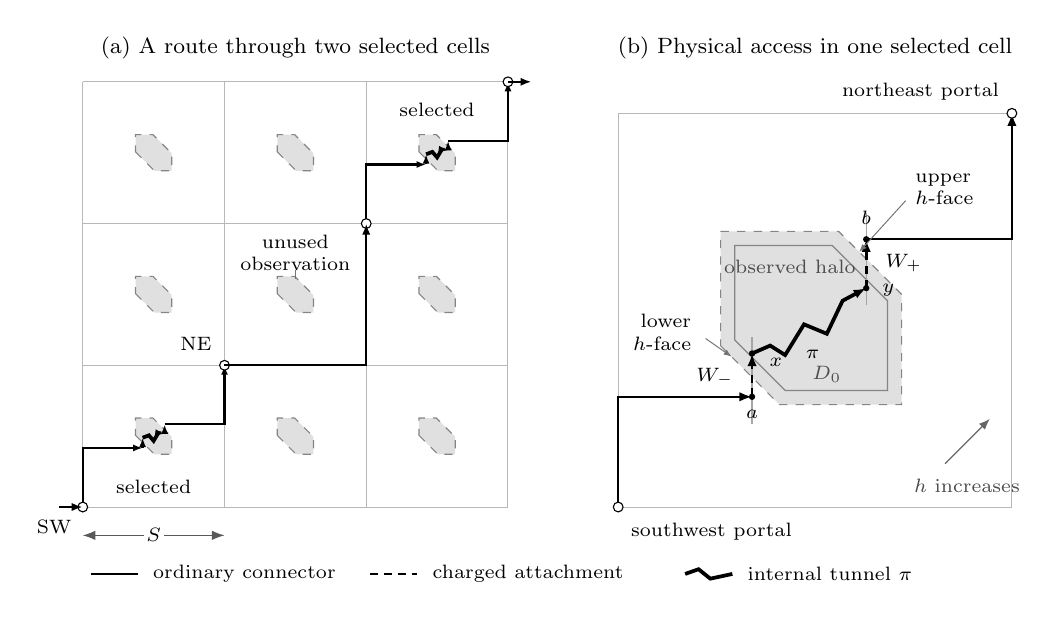
\begin{tikzpicture}[x=1cm,y=1cm,>=Latex,
  every node/.style={font=\scriptsize},
  grid road/.style={draw=black!28,line width=.35pt},
  ordinary/.style={draw=black,line width=.8pt},
  charged/.style={draw=black,line width=1pt,densely dashed},
  tunnel/.style={draw=black,line width=1.35pt},
  halo/.style={draw=black!48,fill=black!12,dashed,line width=.4pt},
  portal/.style={circle,draw=black,fill=white,inner sep=1.25pt}]

\begin{scope}[shift={(.35,.8)}]
  \node[font=\footnotesize] at (2.7,5.83)
    {(a) A route through two selected cells};
  \foreach \v in {0,1.8,3.6,5.4} {
    \draw[grid road] (\v,0)--(\v,5.4);
    \draw[grid road] (0,\v)--(5.4,\v);
  }
  \foreach \sx/\sy in {0/0,1.8/0,3.6/0,0/1.8,1.8/1.8,3.6/1.8,
                         0/3.6,1.8/3.6,3.6/3.6} {
    \begin{scope}[shift={(\sx,\sy)}]
      \path[halo] (.67,.91)--(.91,.67)--(1.13,.67)--(1.13,.89)
        --(.89,1.13)--(.67,1.13)--cycle;
    \end{scope}
  }
  \foreach \sx/\sy in {0/0,3.6/3.6} {
    \begin{scope}[shift={(\sx,\sy)}]
      \draw[ordinary,-{Latex[length=1.2mm]}]
        (0,0)--(0,.75)--(.76,.75);
      \draw[charged,-{Latex[length=1.2mm]}] (.76,.75)--(.76,.88);
      \draw[tunnel,-{Latex[length=1.2mm]}]
        (.76,.88)--(.84,.91)--(.90,.84)--(.96,.94)--(1.04,.93);
      \draw[charged,-{Latex[length=1.2mm]}] (1.04,.93)--(1.04,1.05);
      \draw[ordinary,-{Latex[length=1.2mm]}]
        (1.04,1.05)--(1.8,1.05)--(1.8,1.8);
      \node[portal] at (0,0) {};
      \node[portal] at (1.8,1.8) {};
    \end{scope}
  }
  \draw[ordinary,-{Latex[length=1.4mm]}]
    (1.8,1.8)--(3.6,1.8)--(3.6,3.6);
  \draw[ordinary,-{Latex[length=1.4mm]}] (-.3,0)--(0,0);
  \draw[ordinary,-{Latex[length=1.4mm]}] (5.4,5.4)--(5.7,5.4);
  \node[anchor=north east] at (-.02,-.04) {SW};
  \node[anchor=south east] at (1.76,1.86) {NE};
  \node[anchor=north] at (.9,.47) {selected};
  \node[anchor=south] at (4.5,4.83) {selected};
  \node[align=center] at (2.7,3.23) {unused\\ observation};
  \draw[black!55,line width=.35pt] (2.7,3.01)--(2.7,2.9);
  \draw[<->,black!65,line width=.35pt] (0,-.36)--(1.8,-.36);
  \node[fill=white,inner sep=1pt] at (.9,-.36) {$S$};
\end{scope}

\begin{scope}[shift={(7.15,.8)}]
  \node[font=\footnotesize] at (2.5,5.83)
    {(b) Physical access in one selected cell};
  \draw[grid road] (0,0) rectangle (5,5);
  \path[halo] (1.3,2.05)--(2.05,1.3)--(3.6,1.3)--(3.6,2.7)
    --(2.8,3.5)--(1.3,3.5)--cycle;
  \draw[black!48,line width=.45pt]
    (1.48,2.12)--(2.12,1.48)--(3.42,1.48)--(3.42,2.62)
    --(2.72,3.32)--(1.48,3.32)--cycle;
  \node[black!70] at (2.65,1.68) {$D_0$};
  \node[black!70] at (2.18,3.05) {observed halo};
  \draw[black!35,line width=.45pt] (1.7,1.06)--(1.7,2.16);
  \draw[black!35,line width=.45pt] (3.15,2.56)--(3.15,3.73);
  \draw[ordinary,-{Latex[length=1.6mm]}]
    (0,0)--(0,1.4)--(1.7,1.4);
  \draw[charged,-{Latex[length=1.6mm]}] (1.7,1.4)--(1.7,1.95);
  \draw[tunnel,-{Latex[length=1.6mm]}]
    (1.7,1.95)--(1.93,2.05)--(2.12,1.93)--(2.36,2.32)
    --(2.65,2.2)--(2.85,2.62)--(3.15,2.78);
  \draw[charged,-{Latex[length=1.6mm]}] (3.15,2.78)--(3.15,3.4);
  \draw[ordinary,-{Latex[length=1.6mm]}]
    (3.15,3.4)--(5,3.4)--(5,5);
  \node[portal] at (0,0) {};
  \node[portal] at (5,5) {};
  \foreach \px/\py in {1.7/1.4,1.7/1.95,3.15/2.78,3.15/3.4}
    \fill (\px,\py) circle (1.15pt);
  \node[anchor=north west] at (.04,-.08) {southwest portal};
  \node[anchor=south east] at (4.96,5.04) {northeast portal};
  \node[anchor=north] at (1.7,1.35) {$a$};
  \node[anchor=west] at (1.8,1.84) {$x$};
  \node[anchor=west] at (3.23,2.75) {$y$};
  \node[anchor=south] at (3.15,3.46) {$b$};
  \node[anchor=north] at (2.47,2.12) {$\pi$};
  \node[anchor=east] at (1.59,1.65) {$W_-$};
  \node[anchor=west] at (3.27,3.1) {$W_+$};
  \node[anchor=east,align=right] at (1.05,2.22)
    {lower\\ $h$-face};
  \draw[black!55,-{Latex[length=1mm]},line width=.35pt]
    (1.11,2.14)--(1.44,1.91);
  \node[anchor=west,align=left] at (3.65,4.03)
    {upper\\ $h$-face};
  \draw[black!55,-{Latex[length=1mm]},line width=.35pt]
    (3.65,3.89)--(3.06,3.24);
  \draw[-{Latex[length=1.4mm]},black!60,line width=.45pt]
    (4.15,.55)--(4.72,1.12);
  \node[black!70,anchor=north] at (4.43,.48) {$h$ increases};
\end{scope}

\draw[ordinary] (.45,-.05)--(1.05,-.05);
\node[anchor=west] at (1.12,-.05) {ordinary connector};
\draw[charged] (4,-.05)--(4.6,-.05);
\node[anchor=west] at (4.67,-.05) {charged attachment};
\draw[tunnel] (8,-.05)--(8.17,.01)--(8.32,-.11)--(8.6,-.05);
\node[anchor=west] at (8.67,-.05) {internal tunnel $\pi$};
\end{tikzpicture}
\caption{Physical routing through selected cells, schematically and not to
scale. Gray regions represent observed input halos, including observations
at unused cells. The ordinary connectors have input supports disjoint from
every observed halo. The two dashed attachments at a selected tunnel are
also physical forward portions; their supports may meet only that cell's
observation. In the enlarged cell, the inner outline is $D_0$, the exterior
entry $a$ is below the lower
observed $h$-face and the exterior exit $b$ is above the upper face. The
transverse connectors can therefore reach them without meeting the
observation. The internal path is $\pi:x\to y$. Only physical route portions
are drawn: the signed center-label terms in $H(\pi)$ are bookkeeping and do
not prescribe additional traversals.}
\label{fig:observed-halos-corridors}
\end{figure}

The construction works for every allowed incoming and outgoing label.
After conditioning on all observations, the selected labels and nominal
itineraries are fixed, whereas their actual road geometry and
intersection occurrences remain random.  For each itinerary, use the
envelopes over its full prescribed crossing windows.  Its uncharged
support avoids all observations, so those envelopes retain their
unconditional means.  The mean bound is uniform over the finite label
list and therefore also applies to the observation-dependent choice.

\begin{proposition}[Uniform finite-volume collection bound]
\label{access:collection}
For the iid tunnel field associated with any fixed local type and phase
template there are constants $C,C_0<\infty$, independent of $n$ and the
input-road rule, such that the following holds.  Let $G_n(L)$ be the
maximum of $\sum_{p\in\Gamma}Y_p$ over finite distinct chains in an
arbitrary deterministic translated coordinate square of side at most
$L$, whose consecutive differences have both coordinates at least $2S$.
The empty chain and singletons are allowed.  Then
\begin{equation}\label{access:finite-volume}
                       \E G_n(L)\le CL+C_0.
\end{equation}
The same bound therefore holds if consecutive differences are additionally
required to lie in any fixed inner cone of the positive quadrant.
\end{proposition}

\begin{proof}
\emph{Choose the chain and realize its route.}
Observe the inputs of every test in the sparse array.  In the given
finite square, choose a reward-maximizing chain, resolve ties
lexicographically, and omit zero-reward sites.  This is a function of the
observations.  Fix an
external southwest and an external northeast corridor intersection,
outside the square by $3S$ in both coordinates, with the same prescribed
intersection-label convention.  These endpoints depend on the square,
not on the observed chain.

Route monotonically on the corridor grid from the start to the southwest
portal of the first selected cell, use that tunnel and its private access,
then continue from its northeast portal to the next southwest portal.
The assumed $2S$ gaps make both coordinates of each latter displacement
nonnegative, with a full corridor spacing to spare.  Continue similarly
to the fixed end.  Every portion is a physical forward road portion or a
physical internal tunnel path.  Thus the result is an actual path.

Its total ordinary-corridor length is $O(L+S)$, by telescoping the two
positive coordinate increments.  A chain has at most $C(L/S+1)$ sites.
The private uncharged connector lengths are $O(S)$ per site, so their
total length is also $O(L+S)$.  The number of road switches has the same
bound when measured in unit road spacings.  The two short charged
attachments at each site are excluded from this count.

All selected route costs are integrable. A used tunnel has $Y>0$ and
therefore has negative center-label cost. Rearranging that cost identity
bounds its positive physical passage cost by a bounded $nh$ displacement
and the integrable local gauge and raw-arm envelopes. Charged attachments
and ordinary finite road portions are integrable by the same window
estimates. The chain is finite, and its maximum reward is integrable by
the bound following \eqref{access:charge}. Thus the conditional costs
and the expectation rearrangements below are finite.

\emph{Take conditional expected costs.}
For every prescribed ordinary connector, its full input support misses
\emph{all} observations.  Its inputs therefore retain their product law
under the conditioning.  Subdivide the connector into unit road periods
and apply the local envelopes to those periods and its switches.  Its
expected normalized corrected cost is at most a constant times its
nominal length plus its number of switches.  Summing uses only linearity
of conditional expectation; connectors may share unobserved inputs.

The support of a charged access envelope meets no observation other
than its own test.  Independence gives
\[
 \E[U_{c_-}+U_{c_+}\mid\hbox{all observations}]
 =\E[U_{c_-}+U_{c_+}\mid\mathcal F_{\mathcal D_p}].
\]
Thus each selected tunnel together with its charged attachments has
conditional expected normalized corrected cost at most $-Y_p$, by
Lemma~\ref{access:accounting}.  Consequently the completed path $\Pi$
satisfies
\begin{equation}\label{access:conditional-route}
 \E\left[\frac{Q_n(\Pi)-\Delta g(\Pi)}{\beta}
           \,\middle|\,\hbox{all observations}\right]
                 \le C(L+S)-G_n(L).
\end{equation}

\emph{Apply the calibration at the fixed endpoint windows.}
Corrected costs use only differences of gauges. For this endpoint
calculation, undo any common deterministic centering and use the
original mean-matching gauge representatives; the corrected cost of
$\Pi$ is unchanged.
The constructed path has endpoint labels prescribed by translated copies
of the exterior anchor convention.  Calibration domination gives,
pathwise,
\[
 Q_n(\Pi)-\Delta g(\Pi)
 \ge (P_n-g)(x_{\mathrm{end}})-(P_n-g)(x_{\mathrm{start}}).
\]
Although an endpoint intersection is random, it lies in a prescribed
bounded road window.  Put $R_W=P_n-g_W$ on that exterior road and choose
a fixed marked anchor $k$ before the entire window of possible endpoint
occurrences $t$.  Equation~\eqref{found:eq-mean} gives
$\E R_W(k)=0$, and the defect and interpolation identities give
\[
 R_W(t)-R_W(k)=-D_W(k,t)+C_W(k,t).
\]
The interval is covered by a fixed number of complete road periods.
Additivity and nonnegativity bound its defect by the defects of those
periods; Lemma~\ref{found:lem-envelope} controls its corrected cost.
Thus the expected supremum of the absolute right side is at most
$C\beta$.  In particular,
\[
 \bigl|\E(P_n-g)(x_{\mathrm{start}})\bigr|
 +\bigl|\E(P_n-g)(x_{\mathrm{end}})\bigr|
 \le C\beta.
\]
The estimate covers every possible intersection occurrence and allowed
endpoint label.  Consequently the expected normalized corrected cost of
$\Pi$ is at least $-C$.  Taking expectations in
\eqref{access:conditional-route} yields
$\E G_n(L)\le C(L+S)+C$, and the fixed $S$ is absorbed into $C_0$.
The bound holds at each finite $L$, uniformly over the tunnel law; no
law-dependent limiting passage is needed.
\end{proof}

The constants in Proposition~\ref{access:collection} may depend on the
fixed type, mesh, and sparse spacing, and are uniform over all $n$ and
road rules satisfying the local input assumptions.  Taking their maximum
over the finite type list gives one bound for that list.  For rational
$v,w$ in fixed sufficiently small neighborhoods of the flat endpoints,
the coordinate comparisons and the positive rates $h(A),h(B)$ have
uniform bounds.  The domains, support buffers, and sparse spacing can
therefore be fixed throughout those neighborhoods.  In the application
in Section~\ref{links:section}, this test family is fixed before the
final thin-diagram cone is narrowed.  Rational direction denominators
affect only the divisibility required of $n$.

Together with the phase-template domination, the proposition supplies
the iid collection bounds required by Lemma~\ref{probability:thin-tails}.
The observation domains, candidate shells, and corridors enter this
distributional proof; they do not enlarge the input support of the final
road-improvement rule.

\section{Horizontal links extracted from a long geodesic}
\label{links:section}

The aim is to bound the capped mean cost of a local horizontal crossing.
A long geodesic toward an endpoint of the putative flat has negligible
raw excess.  We extract many crossings from it, control the cost lost
at exceptional pieces by the charged-tunnel estimates, and use row
concentration to compare the surviving sum with a single-link capped mean.
The last step requires two truncation estimates, proved separately below.
Only extremality of the endpoint is used in this extraction.

Costs remain in lattice units, while positions belong to
$\mathcal G_n=n^{-1}\mathbb Z^2$.  Put $d=1-s^2$, and use coordinates $(u,y)$
in the basis $(v,B)$; thus $A=(d,s)$ and $B=(0,1)$.
Tracking and radius-$10$ locality are still measured in the fixed
$(v,w)$ maximum norm.  For $s<1/4$, changes to either
$(v,B)$ or $(A,B)$ coordinates and back cost a factor at most
$2$.  Thus a $B$-wall stays within $2r$ of its nominal line
in the present coordinates.  Lattice-edge rounding errors are at
most $2K_{\rm lat}/n$ in this norm and are absorbed by taking $n$ large.

Constants may depend on the fixed flat.  Those subscripted by
$s$ or $K$, and the large constants used only in the proof, may
also depend on the indicated auxiliary parameters.  The dependence
radius of a link is fixed independently of all truncation and
coarse-graining choices.

\subsection{The signed link and its translation conventions}

Let $W_j$ be the $B$-road with nominal line
$\{(jd,js+t):t\in\mathbb R\}$.  We keep its ordered occurrence
labels, so two visits to one lattice vertex remain distinct.
The nominal parameter is continuous and nondecreasing, and a fixed
first-occurrence convention selects its marked cuts.  This convention
also selects a unique cut at a pause, where the occurrences retain
their order.  The road is locally finite.

Write $R_j(t,t')$ for the signed raw $Q_n$-cost between the
indicated occurrences at $t$ and $t'$.  Reversing the arguments
negates this bookkeeping quantity; a physical reverse traversal has
its own positive passage cost.  With the interpolated local gauge
$g_j$, put
\[
 C_j(t,t')=R_j(t,t')-g_j(t')+g_j(t).
\]
Signed costs are additive in occurrence labels.  Interpolation gives
\[
 C_j(t,t')=(t'-t)C_j(\kappa,\kappa+1),
 \qquad \kappa=\phi_j+m,\quad m\in\mathbb Z,
\]
for occurrences in the marked wall period
$[\kappa,\kappa+1]$, with the relative wall phase $\phi_j$ from
Section~\ref{phases:section}.  This includes pauses.  Longer
intervals are split at the actual marked levels.

Fix a rational row spacing $\sigma<s/1000$, chosen so that $s$ and
all later row offsets are integral multiples of $\sigma$.  Write
$y_k=k\sigma$, $b=s/50$ and $b'=s/20$.  Let $c_{j,k}$ be the
center occurrence of $W_j$ with nominal height $y_k$, that is with
wall parameter $t=y_k-js$, selected by the first-occurrence convention.
An admissible crossing from $W_j$ to $W_{j+1}$ at row $k$ is a finite
physical path $\gamma$, with endpoint occurrences $x\in W_j$ and
$x'\in W_{j+1}$, such that
\begin{enumerate}
\item every point has $|y-y_k|\le b$ and
$jd-b'\le u\le(j+1)d+b'$;
\item for any two points in their traversal order, their horizontal
coordinates satisfy $u_2\ge u_1-b'$.
\end{enumerate}
The second condition bounds every horizontal drawdown along the
crossing, including one that occurs after an earlier visit to the
terminal wall.  At finite $n$, round the band boundaries outward to
the nearest lattice boundaries; the $O(1/n)$ error fits inside the
strict margins used below.  Equivalently, fix rational padded
boundaries and require sufficient divisibility of $n$.
Measure the crossing at the two row centers by setting
\begin{align}
 L_{j,k}(\gamma)
  &=C_j(c_{j,k},x)
    +Q_n(\gamma)-g_{j+1}(x')+g_j(x)
    +C_{j+1}(x',c_{j+1,k}), \\
 X_{j,k}&=\min_\gamma L_{j,k}(\gamma).
 \label{links:definition}
\end{align}
The closed-window endpoint-selection argument preceding
Lemma~\ref{found:lem-envelope} gives an attained measurable local
minimum. The band and all-pairs drawdown conditions are closed and
survive loop deletion. The class is nonempty for large $n$: follow the horizontal center line by a
lattice path and retain the portion between appropriate consecutive
crossings of the two proper vertical roads.  The planar
rectangle-crossing property ensures these intersections even when
the roads have self-intersections.

When a link is used in a new road, its minimizer may be chosen with
vertex endpoints. For a loop-erased minimizer starting at an interior
point $x$ of a wall edge, let $v$ be the first adjacent vertex reached
by the crossing. Delete the partial prefix from $x$ to $v$ and move
the wall attachment to the corresponding occurrence of $v$. The change
in the center-adjusted cost is
\[
 R_j(x,v)-Q_n(x\mathbin{\to}v)
 =\begin{cases}
 0,&\text{if the partial traversal follows the wall},\\
 -2\tau(x\mathbin{\to}v),&\text{if it reverses the wall}.
 \end{cases}
\]
The right endpoint has the same property after deleting its final
partial edge. The two walls have positive separation, so for large
$n$ these deletions are disjoint. The remaining subpath retains the
band and drawdown conditions. Its cost cannot exceed the minimum and
therefore equals it. Choose the first such vertex-ended minimizer in
the relative order above. This supplies a lattice path at every link
splice, while the definition still compares all allowed interior
attachments.

The minimum has a uniform bound on its negative first moment:
Lemma~\ref{found:lem-envelope} gives
\begin{equation}
 \mathbb E(X_{j,k})^-\le C\beta.
 \label{links:negative-moment}
\end{equation}
To see why taking a minimum causes no loss, apply calibration
domination to each physical $\gamma$.  After taking the difference
between the two center labels, the endpoint calibration--gauge
discrepancies have $L^1$ suprema at most $C\beta$.  The two
interpolated center arms obey the same bound.  Their suprema provide
one lower bound valid for all competitors before minimization.
The calibration enters this estimate; the definition of $X_{j,k}$
uses only local inputs.  The constant $C$ is independent of small
$s$, the row mesh, and the input rule, because only two labels and
bounded parameter windows are compared, and finite averaging of
gauges preserves these bounds.

The same first-moment proof applies with every phase entering the link
and its gauge projections fixed. The calibration depends only on the
edges, while the local-envelope proof treats phases as parameters and
uses period, interpolation, and projection bounds uniform over their
admissible assignments. Thus a link \(X^t\) evaluated under any fixed
local phase template of Section~\ref{access:phases} satisfies
\begin{equation}
 \mathbb E[(X^t)^-]\le C\beta.
 \label{links:fixed-phase-negative-moment}
\end{equation}
This fixed-phase form will be used for the sparse negative-link flags.

Two properties of the phase construction will turn selected sums
into a statement about one link.  Use Lemma~\ref{phases:locality}
with $\mathcal H$ containing $s$, $\sigma$, and all required row
offsets.  Translation by $d v=A-sB$ advances a column at fixed
height; translation by $\sigma B$ advances a row.  Covariance of
the phases and averaged gauges therefore gives every $X_{j,k}$
the same law, denoted by $X$.  The lemma also gives a fixed integer
$q$ for which entire-column sigma-fields with indices in one residue
class modulo $q$ are mutually independent.  These are precisely
the stationarity and independence used in Lemma~\ref{probability:rows}.
For a finite family of crossing templates, apply this construction
and the extraction separately to each template.

\subsection{The geometric extraction}

Two geometric facts are needed. Near-minimal norm length forces most
fine increments toward the extreme endpoint. At the coarser scale,
deleting neighborhoods of bad pieces gives the all-pairs order required
by the tunnel-tail estimate. Write
\[
 \mathcal C=\{z:\mu(z)=h(z)\}
\]
for the cone on the flat, and choose pointed closed cones with
\[
 \mathcal C\setminus\{0\}\subset\operatorname{int}\mathcal C_1,
 \qquad
 \mathcal C_1\setminus\{0\}\subset\operatorname{int}\mathcal C_2.
\]
They can be arbitrarily close to \(\mathcal C\). On every such cone
sufficiently close to \(\mathcal C\), \(h(z)\ge c|z|\), with \(c>0\)
independent of the enlargement.

\begin{lemma}[A uniform modulus at an extreme point]
\label{links:extreme}
Let \(a\) be an extreme point of the norm ball, let
\(S_\mu=\{z:\mu(z)=1\}\), and let \(U\) be a relatively open
neighborhood of \(a\) in \(S_\mu\). For \(t\ge0\), put
\[
 \omega_U(t)=\sup\left\{\nu(S_\mu\setminus U):
    \nu\in\mathcal P(S_\mu),\
    \left|\int z\,d\nu(z)-a\right|\le t\right\}.
\]
Then \(\omega_U(t)\to0\) as \(t\downarrow0\). If \(N>0\),
\(0\le d_0<1/2\), and finitely many increments satisfy
\[
 \left|\sum_i z_i-Na\right|\le d_0N,\qquad
 \left|\sum_i\mu(z_i)-N\right|\le d_0N,
\]
then, with \(C_a=2(1+|a|)\),
\begin{equation}
 \sum_{i:z_i/\mu(z_i)\notin U}\mu(z_i)
 \le (1+d_0)N\,\omega_U(C_a d_0).
 \label{links:extreme-modulus}
\end{equation}
Zero increments are omitted. In particular, endpoint error \(o(N)\)
and total norm length \(N+o(N)\) imply \(o(N)\) norm mass outside \(U\).
\end{lemma}

\begin{proof}
Put \(F=S_\mu\setminus U\). If the first assertion failed, there
would be \(t_j\downarrow0\) and probability measures \(\nu_j\) with
barycenters within \(t_j\) of \(a\) and \(\nu_j(F)\ge e>0\).
A weakly convergent subsequence exists on the compact sphere. Its
limit \(\nu\) has barycenter \(a\), and the closed-set inequality
gives \(\nu(F)\ge\limsup_j\nu_j(F)\ge e\).

The convex hull of \(F\) is compact and omits \(a\). Indeed,
Carath\'eodory's theorem would otherwise express \(a\) as a finite
nontrivial convex combination of points different from \(a\),
contrary to extremality. If \(\nu(F)=1\), its barycenter lies in that
convex hull. If \(0<\nu(F)<1\), the conditional barycenters on \(F\)
and its complement lie in the norm ball and express \(a\) as a
nontrivial convex combination. Extremality makes both equal to \(a\),
whereas the first lies in the convex hull of \(F\). Both cases are
impossible, proving \(\omega_U(t)\to0\).

For the second assertion put \(S=\sum_i\mu(z_i)>0\) and give
\(z_i/\mu(z_i)\) mass \(\mu(z_i)/S\). Its barycenter is
\((\sum_i z_i)/S\), at distance at most
\[
 \frac{d_0+d_0|a|}{1-d_0}\le C_a d_0
\]
from \(a\). The mass on \(F\), multiplied by \(S\le(1+d_0)N\),
is the left side of \eqref{links:extreme-modulus}.
\end{proof}

Deleting only the bad indices would not control an interval that
crosses several of them. The next lemma removes a density halo:
every interval touching a retained index then contains enough good
increments to enforce forward order. The raw penalty on bad indices
pays for all removed effective gauge differences.

\begin{lemma}[Removal of bad intervals]
\label{links:halos}
Let \(x_0,\ldots,x_m\) be successive cuts of a path. All distances
in this lemma use the \((A,B)\) maximum norm. Suppose
\(K/2\le|x_{i+1}-x_i|\le CK\), and associate to each starting cut
\(x_i\) a center \(z_i\) within a fixed distance \(H_0\), independent
of the cone enlargement. Declare an index bad when its
increment is outside \(\mathcal C_1\), or its physical subpath has
a backward \(h\)-excursion of size at least one. Suppose, for
\(c_*>0\) and \(\epsilon_n^{\rm raw}\to0\), its raw costs satisfy
\[
 Q_i\ge-\epsilon_n^{\rm raw}n\quad\hbox{for all }i,
 \qquad Q_i\ge c_*n\quad\hbox{for bad }i.
\]
Let effective cut labels satisfy
\(|\widetilde g_i-g_{\rm ref}|\le\lambda n\) for one common constant
\(g_{\rm ref}\). For sufficiently small \(\lambda>0\) there is a set
\(R\) of removed indices containing all bad indices, of cardinality
at most a fixed multiple of their number, for which
\begin{enumerate}
\item \(\sum_{i\in R}(Q_i-\widetilde g_{i+1}+\widetilde g_i)\ge0\);
\item retained centers \(z_i\) are in \(\mathcal C_2\)-order up to a bounded
additive error, for every pair of retained indices;
\item the same order includes the initial and terminal points, up to
a bounded additive error;
\item repetitions of any one center have bounded multiplicity, independently of how
small the cone enlargement is.
\end{enumerate}
\end{lemma}

\begin{proof}
Let \(B_0\) be the bad set. For \(\theta>0\), put
\[
 R=\{i:\text{some index interval }I\ni i
                    \text{ has }|I\cap B_0|>\theta|I|\}.
\]
A one-dimensional maximal-interval bound gives
\(|R|\le3|B_0|/\theta\): select disjoint witness intervals in
decreasing order of length. Their triple enlargements cover all
discarded witness intervals, and their lengths sum to at most
\(|B_0|/\theta\). Every interval containing a retained index
therefore has bad density at most \(\theta\).

Let \(\ell_1,\ell_2\) be the coordinate functionals of
\(\mathcal C_2\). Compactness and the strict cone inclusion give
\(\ell_j(x_{i+1}-x_i)\ge\kappa_0K\) at good indices, whereas at bad
indices they are at least \(-CK\). Choose
\(\theta<\kappa_0/(2(C+\kappa_0))\). Every interval containing a
retained index then satisfies
\[
 \ell_j\left(\sum_{i\in I}(x_{i+1}-x_i)\right)
                      \ge\tfrac12\kappa_0K|I|.
\]
Apply this to the interval between two retained cut indices, then
absorb the bounded errors in choosing their centers. To include the
initial endpoint and a retained starting-cut representative \(x_i\),
use the prefix through increment \(i\) and subtract that increment,
whose size is at most \(CK\). The suffix from \(x_i\) already contains
the retained index. Center rounding adds another bounded error.
The coordinate matrices range in a fixed compact set, so these errors
remain uniform as the cone enlargement shrinks.

For multiplicity, apply the same density argument to \(h\). After
decreasing \(\theta\) if necessary, it gives
\(h(x_j-x_i)\ge cK(j-i)\) on the relevant intervals, where \(c\) is
independent of the cone enlargement. Only boundedly many retained
centers can therefore lie in any fixed-radius ball.

For the cost assertion, bound each removed gauge difference separately:
\begin{align*}
 \sum_{i\in R}(Q_i-\widetilde g_{i+1}+\widetilde g_i)
 &\ge n\{c_*|B_0|-(\epsilon_n^{\rm raw}+2\lambda)|R|\}\\
 &\ge n\left\{c_*-\frac{3(\epsilon_n^{\rm raw}+2\lambda)}{\theta}\right\}|B_0|.
\end{align*}
Choose \(\lambda<c_*\theta/24\) and then \(n\) large. The bracket is
at least \(c_*/2\), retaining a positive penalty per bad index.
The set \(R\) depends only on the bad indices, so this conclusion
holds for every assignment of effective gauges satisfying the stated
bound.
\end{proof}

\paragraph{Costs at shared cuts.}
For an allowed road label \(W\), a cut occurrence \(x\), and a
permitted datum \(\bar x\) on the same wall, define
\begin{equation}
 \widetilde g_W(x;\bar x)=g_W(\bar x)+R_W(\bar x,x).
 \label{links:effective-gauge}
\end{equation}
The datum is a prescribed row center or reference center in the
bounded windows of the access construction. At a shared cut \(x_i\),
both incident pieces will use one datum \(\bar x_i\). Writing
\(\widetilde g_i=\widetilde g_{W_i}(x_i;\bar x_i)\), define
\begin{align}
 c_i^{\rm cost}
 &=\beta^{-1}\{C(\bar x_i,x_i)+Q_n(\gamma_i)
       -g(x_{i+1})+g(x_i)+C(x_{i+1},\bar x_{i+1})\}\notag\\
 &=\beta^{-1}\{Q_n(\gamma_i)-\widetilde g_{i+1}+\widetilde g_i\}.
 \label{links:piece-cost}
\end{align}
The second equality is additivity of signed wall costs. The cut
selection takes its suprema over every allowed label, cut occurrence,
and future datum before any row is chosen. Lemma~\ref{found:lem-gauge-tail}
therefore bounds all the effective gauges in
\eqref{links:effective-gauge} relative to one deterministic reference
mean for the law and scale.

\subsection{Uniform extraction}

We state the output shared by the two capped estimates. For the final
fixed rational directions, let \(\mathfrak R_n\) be the class of
admissible input-road laws with
\[
 c_0\le\beta\le C_s n^\alpha,\qquad \alpha<1,
\]
where these constants are fixed as the law and \(n\) vary. The
preceding local, selected-cut, and collection estimates apply
uniformly to this whole class.

The order of choices is as follows. Fix \(s,\sigma\), the local access
construction, and \(\chi=0.99\). Choose an integer \(L>99\), put
\(N=n^L\), and take \(m=m_*>4\) in Lemma~\ref{access:selected-cuts}
with \(m_*\vartheta>2L+10\). Retain its radii \(H_m\) and \(K>20H_m\);
\(K\) is the actual preliminary exit radius. Fix the finite tunnel
types and their collection constants in one larger cone. The capped
proofs then choose \(F,T\), their caps or finite cap menu, and all
entropy tolerances. For their requested thin width \(\delta\) and
row tolerance \(\eta\), choose the final cones, the halo parameters
\(\theta,\lambda\), the fine cone and radius, and the rational
direction errors. Finally impose divisibility and take \(n\) large.
The constants multiplying \(\eta\) below are fixed before \(\eta\);
later fine and cone choices enter the error sequence. The finite phase
lists are independent of the eventual direction denominators, as
explained in Section~\ref{phases:section}. These proof parameters
never enlarge the input support of an individual link.

\begin{proposition}[Uniform extraction from a long geodesic]
\label{links:extraction}
For every sufficiently small fixed \(\delta,\eta>0\), the final
geometric choices above can be made so that there are deterministic
\(\epsilon_n,\pi_n\to0\) and fixed constants \(H,C,C_K,c>0\) and
integers \(q_K,m_0\) with the following property. For each
\(\mathfrak r\in\mathfrak R_n\) there is an event \(\Omega_{n,\mathfrak r}\)
such that
\begin{equation}
 \sup_{\mathfrak r\in\mathfrak R_n}
 \mathbb P_{\mathfrak r}(\Omega_{n,\mathfrak r}^{\,c})\le\pi_n.
 \label{links:extraction-event}
\end{equation}
Let \(x_n^\star\) be a deterministic nearest vertex of \(\mathcal G_n\)
to \(Na\), and put
\[
 j_n=\left\lfloor u(x_n^\star)/d+\tfrac12\right\rfloor,\qquad
 \mathcal J_n=\{0,1,\ldots,j_n-1\}.
\]
For large \(n\), \(cN\le j_n\le CN\). On \(\Omega_{n,\mathfrak r}\),
a geodesic from \(0\) to \(x_n^\star\) has consecutive selected pieces
\(\gamma_i:x_i\to x_{i+1}\), \(0\le i<m_N\), after two bounded terminal
fragments are removed, and the following objects and bounds.
\begin{enumerate}
\item There are at most \(CN/K+C\) pieces, each of diameter \(O(K)\),
with consecutive cut displacement between \(K/2\) and \(2K\) in the
\((A,B)\) maximum norm. The shared data in
\eqref{links:piece-cost} have
\(|\widetilde g_i-g_{\rm ref}|\le\lambda n\). A removed set \(R\)
contains every bad piece of Lemma~\ref{links:halos} and satisfies
\begin{equation}
 |R|\le\epsilon_nN,\qquad
 \sum_{i\in R}c_i^{\rm cost}\ge0,\qquad
 \sum_{i\notin R}c_i^{\rm cost}\le\epsilon_nN.
 \label{links:retained-cost}
\end{equation}

\item The retained pieces have types \(t_i\) from the fixed access
family and centers \(z_i\) on its fixed finite family of full-rank
center lattices, after bounded rounding. Let \(E=[e_1\ e_2]\), where
the \(e_j\) are the boundary generators of \(\mathcal C_2\), normalized
by \(h(e_j)=1\) and ordered so that \(e_1\to a\) and \(e_2\to b\)
as \(\mathcal C_2\) shrinks to \(\mathcal C\). In
chronological order the centers satisfy
\begin{equation}
 E^{-1}(z_j-z_i)\ge-H(1,1)\quad(i<j),\qquad
 z_i\in E([-H,CN+H]\times[-H,\delta N+H]).
 \label{links:retained-geometry}
\end{equation}
The inequality is coordinatewise. Each rounded site occurs at most
\(m_0\) times, and the initial distance from the origin plus total
successive center distance is at most \(C(N+1)\). These bounds persist
on every type and sparse-residue subsequence. The matrices \(E\) range
in a fixed compact family, and \(H,C,m_0\) remain bounded when the
final cone is narrowed.

\item An irregular retained set \(\mathcal I\) has
\(|\mathcal I|\le(C_K\eta+\epsilon_n)N\). Each
\(i\notin R\cup\mathcal I\) supplies at most \(q_K\) admissible links
\(\mathcal L_i\), with
\begin{equation}
 c_i^{\rm cost}\ge\sum_{(j,k)\in\mathcal L_i}X_{j,k}/\beta.
 \label{links:unclipped-comparison}
\end{equation}
In the chronological list
\(\mathcal L=\bigcup_{i\notin R\cup\mathcal I}\mathcal L_i\), columns
are distinct, increasing, and belong to \(\mathcal J_n\). For
sufficiently small fixed \(\eta\), \(|\mathcal L|\ge cN\) for all
large \(n\), after decreasing \(c\) once. If \(k_1,\ldots,k_\ell\)
are the selected rows, then
\begin{equation}
 \begin{gathered}
 |\mathcal J_n\setminus\{j:(j,k)\in\mathcal L\}|
       \le(C_K\eta+\epsilon_n)N,\qquad |k_1|\le j_n^2,\\
 \sum_{\nu<\ell}|k_{\nu+1}-k_\nu|
       \le(C_K\eta+\epsilon_n)N.
 \end{gathered}
 \label{links:selected-rows}
\end{equation}
Rows can be held across omitted columns without increasing their variation.

\item Every retained piece obeys the charged-tunnel bound
\begin{equation}
 (c_i^{\rm cost})^-\le Y_{z_i,t_i}+E_{z_i}.
 \label{links:tunnel-bound}
\end{equation}
Here \(Y\) is the local saving of Section~\ref{access:tunnels}, and
\(E\) is a fixed local sum at the piece center that dominates both
selected endpoint errors for every allowed piece. The finite
phase-template fields for \(Y\) satisfy
Proposition~\ref{access:collection}; those for \(E\) have fixed range
and tail \(C_K\min(1,t^{-m_*})\).
\end{enumerate}
Set every selected list and count, including \(m_N,R,\mathcal I,\mathcal L\),
to the empty or zero value off \(\Omega_{n,\mathfrak r}\).
For finitely many link templates, apply the proposition separately,
intersect their events, and take the maximum of their error sequences
and the sum of their failure sequences.
\end{proposition}

\begin{proof}
\emph{An edge-only event and fine directions.}
Choose the nearest endpoint and the geodesic by fixed tie conventions.
The metric and cheap-path estimates give an event \(\mathsf M_n\)
depending only on the edge weights, with
\(\rho_n=\mathbb P_{\rm edge}(\mathsf M_n^c)\to0\), on which
\begin{equation}
 |Q_n(\gamma)|\le q_nN,\qquad |\gamma|_{\rm edges}\le CNn,\qquad
 \gamma\subset[-CN,CN]^2,\qquad
 q_n=C\frac{(Nn)^\chi+1}{N}\to0.
 \label{links:long-geodesic}
\end{equation}
Here \(L>99\) makes \((Nn)^{0.99}=o(N)\); endpoint rounding contributes
only \(O(1)\) to \(Q_n\). Write \(T_n(x,y)=T(nx,ny)\) for scaled
metric-graph endpoints. On the same event, every such pair in a fixed
enlargement of this box and at the bounded scaled distances used below
satisfies
\[
 T_n(x,y)\ge n\mu(y-x)-e_n,\qquad e_n=C_Kn^\chi=o(n).
\]
The graph-endpoint assertion includes the maximum incident-edge bound
from Lemma~\ref{model:metric}. Thus it holds simultaneously before any
cuts are chosen.

The fine choices in the stated parameter order can be made as follows.
Choose the rational approximation to \(a\), a neighborhood \(U\), and
\(\varepsilon_f>0\) so that every increment directed in \(U\) satisfies
\[
 u(z)\ge0,\qquad |y(z)|\le\varepsilon_f u(z)
                         \le\tfrac12\eta\sigma\,\mu(z).
\]
Indeed \(u(a)>0\), \(y(a)\to0\) as \(v\to a\), and \(u(z)\le C\mu(z)\)
by fixed norm comparison. Take \(\varepsilon_f\) small enough and choose
the fixed radius \(\varrho\) so that
\begin{equation}
 \kappa=s+d\varepsilon_f\le\tfrac12,\quad
 12\varrho<H_m,\quad \varrho<\sigma/100,\quad
 2(1+s)\varrho<b/10,\quad 2r+4d\varrho<b'.
 \label{links:fine-choices}
\end{equation}
These conditions are compatible because \(s<1/4\) and \(2r<b'\).

Use the fine exit partition of radius \(\varrho\) in the \((A,B)\)
maximum norm. Each fine trace has diameter at most \(2\varrho\),
including the final incomplete trace. The edge budget bounds the number
of fine segments by \(CN/\varrho+1\). For their increments \(z_i\), put
\(S_n=\sum_i\mu(z_i)\). Summing the metric lower bounds gives
\[
 nS_n\le nN+C+q_nN+(CN/\varrho+1)e_n,
\]
while the triangle inequality and endpoint rounding give
\(S_n\ge N-C/n\) and \(|\sum_i z_i-Na|\le C/n\). Thus both errors in
Lemma~\ref{links:extreme}, divided by \(N\), are at most
\[
 d_n=C\left(\frac1{nN}+\frac{q_n}{n}
              +\frac{e_n}{n\varrho}+\frac{e_n}{nN}\right)\to0.
\]
Define
\[
 \epsilon_n^{\rm fine}=(1+d_n)\omega_U(C_a d_n)\to0.
\]
The total norm mass outside \(U\) is at most
\(\epsilon_n^{\rm fine}N\). Every full fine increment has norm length
at least \(c\varrho\), so there are at most
\(C\epsilon_n^{\rm fine}N/\varrho+1\) bad increments, including a
possible bad incomplete one. A zero final segment is omitted.
The good transverse variation is at most
\(\tfrac12\eta\sigma S_n\le\eta\sigma N\) for large \(n\), and the bad
variation is at most \(C\epsilon_n^{\rm fine}N\). All these bounds hold
on the same edge event for every road law.

\emph{Cuts and the uniform good event.}
Place the actual preliminary \(K\)-exit marks in the \((A,B)\) maximum
norm. At each mark test every fine interval whose occurrence-time
interval meets the terminal arc, including at either endpoint.
The coordinate identities
\[
 u=d\xi_1,\qquad y=s\xi_1+\xi_2
\]
put every good fine displacement in \(\mathcal G_\kappa\) of
\eqref{access:horizontal-hyp}. With \(\delta_f=2\varrho\),
\(\kappa\le1/2\) and \(12\varrho<H_m\) imply its exact strict
condition
\[
 H_m>\frac{2(1+\kappa)}{1-\kappa}\delta_f.
\]
If every fine interval meeting the terminal arc is good, use the
\(B\)-wall candidates of Lemma~\ref{access:selected-cuts}; otherwise
use its annulus candidates. Both tuple families and all future datum
choices were included before this test in the single objective
\(W_c/\beta+V_c/a_n\).

With \(a_n=C_1n^{1-\vartheta}\), that lemma supplies
\begin{equation}
 \mathbb P_{\mathfrak r}(E_z>t)\le C_K\min(1,t^{-m_*}),\qquad
 W_{\rm cut}/\beta\le E_z,\qquad V_{\rm cut}\le a_nE_z.
 \label{links:joint-cut-bound}
\end{equation}
The inequalities cover every allowed effective gauge at the chosen
cut. Let \(\mathcal Z_n\) be the deterministic set of possible mark
cells in the box of \eqref{links:long-geodesic}, with its fixed
boundary enlargement. It has at most \(Cn^{2L+10}\) cells. Define
\[
 \Omega_{n,\mathfrak r}
   =\mathsf M_n\cap\{\max_{z\in\mathcal Z_n}a_nE_z\le\lambda n\}.
\]
The union bound in the selected-cuts lemma gives
\[
 \mathbb P_{\mathfrak r}(\Omega_{n,\mathfrak r}^{\,c})
 \le \rho_n+C_{\lambda,K}n^{\,2L+10-m_*\vartheta}
 =:\pi_n\longrightarrow0
\]
uniformly in \(\mathfrak r\). No independence between the metric event
and the cut fields is needed. A selected cut lies within \(H_m\) of its
mark. Since successive preliminary displacements equal \(K\), selected
displacements lie between \(K-2H_m\) and \(K+2H_m\), in particular
between \(K/2\) and \(2K\). The intervening pieces and the two terminal
fragments have diameter \(O(K)\).

\emph{The halo and its cost.}
Each terminal fragment has raw cost at least \(-e_n\), so the selected
pieces have total raw cost at most \(q_nN+2e_n\). Every such piece has
raw cost at least \(-e_n\). For an off-\(\mathcal C_1\) displacement
in the fixed annulus, compactness gives a positive lower bound for
\(\mu(z)-h(z)\). For a unit backward \(h\)-excursion, split before,
during, and after the excursion; \(\mu\ge|h|\) gives raw cost at least
\(2n-3e_n\). For some fixed \(c_*>0\), bad pieces therefore cost at
least \(c_*n\) for large \(n\). Let \(B_0\) be their index set.
The edge budget gives at most \(CN/K+C\) pieces, whence
\[
 \frac{|B_0|}{N}
 \le C\left(\frac{q_n}{n}+\frac{e_n}{nK}
                         +\frac{e_n}{nN}\right).
\]
Use the fixed \(\lambda<c_*\theta/24\) from the halo lemma and
\(\epsilon_n^{\rm raw}=e_n/n\). The halo set \(R\) depends only on
\(B_0\), and \(|R|\le3|B_0|/\theta\). On \(\Omega_{n,\mathfrak r}\)
the gauge bound holds simultaneously for every later datum, so the
removed cost is nonnegative for the eventual shared choices. They
telescope on the full consecutive list, giving
\[
 \sum_{i\notin R}c_i^{\rm cost}
 \le\sum_i c_i^{\rm cost}
 \le c_0^{-1}(q_nN+2e_n+2\lambda n).
\]

The halo's endpoint order puts the retained centers in
\eqref{links:retained-geometry}: the second \(E\)-coordinate of \(a\)
tends to zero as \(\mathcal C_2\) shrinks to \(\mathcal C\).
The endpoint and center errors stay bounded because \(E\) ranges in a
compact family. Each preliminary exit uses at least \(cKn\) edges,
so there are \(O(N/K)\) centers. Their successive-distance budget,
including the initial \(O(K)\) distance, is \(O(N)\). The halo lemma
also gives the stated multiplicity bound.

\emph{Rows and regular links.}
Track the fine polygon by hysteresis: keep its current row until it
leaves the central sub-band of half-width \(b/4\), then choose the
nearest row. Since \(\sigma<b/10\), each change except possibly the
first consumes at least \(b/10\) of transverse variation. The row-index
variation is bounded by a constant times that variation divided by
\(\sigma\), plus a constant times the number of changes. It is at most
\[
 C_K\eta N+C_{\rm fixed}\epsilon_n^{\rm fine}N+O(1).
\]
Let \(\mathcal I_0\) contain exactly the pieces whose closed
occurrence-time intervals meet a row change or a bad fine interval,
or which are incident to a failed terminal test. Define this set on
the full selected list, regardless of membership in \(R\).
A row-change time lies in at most two closed coarse intervals.
A fine trace has diameter
at most \(2\varrho\). Its closed occurrence-time interval can meet at most
two closed coarse intervals, since otherwise it contains two consecutive cuts
separated by \(K/2\). Each terminal arc occurs after its preceding
preliminary mark. A fine interval meeting three terminal arcs would
contain two consecutive preliminary marks, separated by \(K\).
Each failed test is incident to at most two pieces and is charged to a
bad fine interval meeting its terminal arc. Thus
\[
 |\mathcal I_0|
 \le C_K\eta N+C_{\rm fixed}\epsilon_n^{\rm fine}N+O(1).
\]

On a piece outside \(\mathcal I_0\), every fine interval meeting it
chronologically is good. The polygon calculation in
\eqref{access:horizontal-submotion}, now applied to any
submotion of this piece with \(\delta_f=2\varrho\), gives horizontal
drawdown at most \(4d\varrho\). The path is within transverse distance
\(2(1+s)\varrho\) of its fine polygon. The hysteresis and
\eqref{links:fine-choices} therefore keep the whole piece in one full
row band, with drawdown less than \(b'\). Its two successful terminal
tests supply \(B\)-wall vertex occurrences.
Write \(k_i\) for this constant hysteresis row. Two adjacent pieces
outside \(\mathcal I_0\) have the same row: their closed time intervals
share a cut, and a change there would put the incident pieces in
\(\mathcal I_0\).

The first \((A,B)\) coordinate increases across this piece. Its
maximum norm displacement is at least \(K-2H_m\). If the negative
first coordinate realized that norm, its size would be at most
\(4\varrho\) by \eqref{access:horizontal-submotion}; if the second
coordinate realized it, its size would be at most
\(4(1+\kappa)\varrho/(1-\kappa)\le12\varrho\).
Both contradict \(12\varrho<H_m<K/20\). Hence the first-coordinate
increase is at least \(K-2H_m\). Since \(\rho=2r\) is the wall tracking
width in these coordinates, the terminal wall index exceeds the initial
one by at least \(K-2H_m-2\rho>0\).

Split the piece at successive first meetings of the next \(B\)-wall.
At each intermediate meeting, use one occurrence of that wall for both
adjoining subpaths.
Planarity forces a meeting before passage beyond that wall's far
padded side, and the drawdown bound for every submotion supplies the
backward allowance. End the final subpath at the original terminal cut,
even if it met that wall earlier. Its overshoot is at most \(2r+4d\varrho<b'\),
so the entire trailing portion is retained. These are admissible links
in \eqref{links:definition}; the piece diameter bounds their number
by a fixed \(q_K\). Write \(q_i\le q_K\) for this number.

Figure~\ref{fig:horizontal-cuts-links} shows the terminal-wall candidates
and the first-meeting decomposition of a regular piece, including its
final subpath after an earlier visit to the terminal wall.

\begin{figure}[t]
\centering
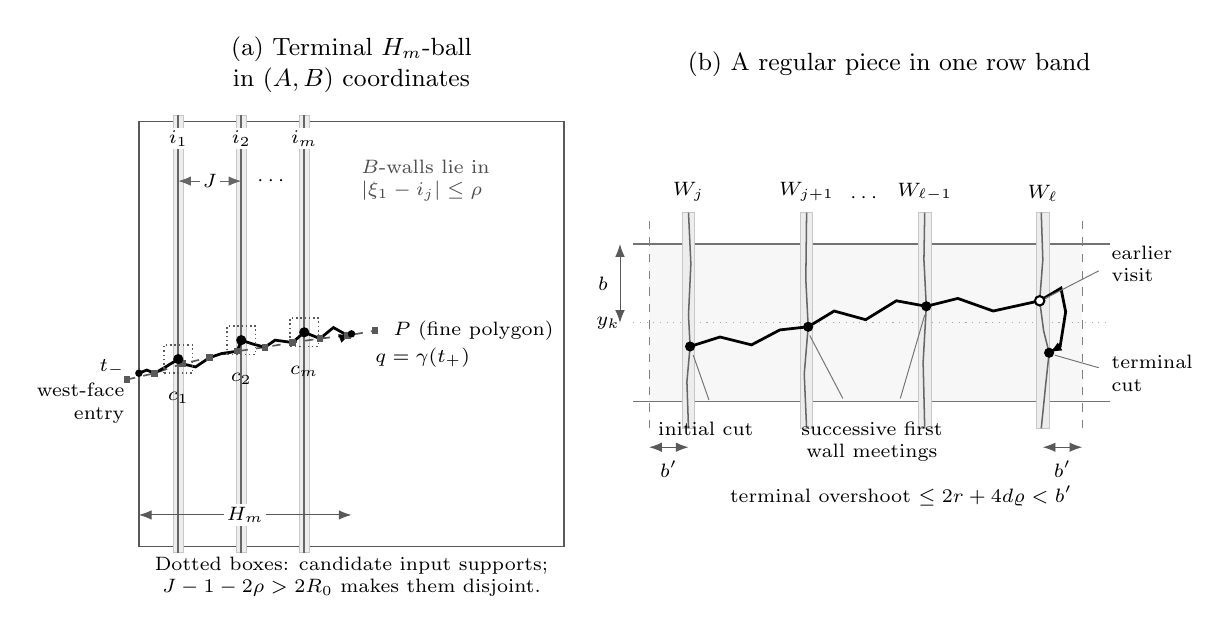
\begin{tikzpicture}[x=1cm,y=1cm,>=Latex,
  every node/.style={font=\scriptsize},
  path trace/.style={draw=black,line width=1pt},
  fine polygon/.style={draw=black!65,dashed,line width=.6pt},
  wall/.style={draw=black!60,line width=.55pt},
  wall strip/.style={fill=black!7,draw=black!22,line width=.3pt},
  support/.style={draw=black!65,densely dotted,line width=.55pt},
  cut/.style={circle,fill=black,inner sep=1.3pt}]

\begin{scope}[shift={(.42,.83)}]
  \node[font=\small,align=center] at (2.7,6.12)
    {(a) Terminal $H_m$-ball\\in $(A,B)$ coordinates};
  \draw[black!65,line width=.5pt] (0,0) rectangle (5.4,5.4);
  \foreach \v in {.5,1.3,2.1} {
    \path[wall strip] (\v-.06,-.08) rectangle (\v+.06,5.48);
    \draw[wall] (\v,-.08)--(\v,5.48);
  }
  \node[fill=white,inner sep=1pt] at (.5,5.18) {$i_1$};
  \node[fill=white,inner sep=1pt] at (1.3,5.18) {$i_2$};
  \node[fill=white,inner sep=1pt] at (2.1,5.18) {$i_m$};
  \draw[<->,black!60,line width=.35pt] (.5,4.64)--(1.3,4.64);
  \node[fill=white,inner sep=1pt] at (.9,4.64) {$J$};
  \node[fill=white,inner sep=1pt] at (1.7,4.64) {$\cdots$};
  \node[anchor=west,align=left,black!70] at (2.7,4.65)
    {$B$-walls lie in\\ $|\xi_1-i_j|\le\rho$};
  \draw[fine polygon]
    (-.15,2.12)--(.2,2.2)--(.55,2.32)--(.9,2.4)--(1.25,2.48)
    --(1.6,2.53)--(1.95,2.59)--(2.3,2.64)--(2.65,2.68)--(3,2.74);
  \draw[path trace,-{Latex[length=1.6mm]}]
    (0,2.2)--(.1,2.24)--(.2,2.2)--(.34,2.28)--(.5,2.38)--(.55,2.32)
    --(.72,2.28)--(.9,2.4)--(1.05,2.45)--(1.25,2.48)--(1.3,2.62)
    --(1.45,2.57)--(1.6,2.53)--(1.73,2.62)--(1.95,2.59)--(2.1,2.72)
    --(2.3,2.64)--(2.47,2.78)--(2.65,2.68)--(2.7,2.7);
  \foreach \px/\py in {-.15/2.12,.2/2.2,.55/2.32,.9/2.4,1.25/2.48,
                         1.6/2.53,1.95/2.59,2.3/2.64,2.65/2.68,3/2.74}
    \draw[fill=white,black!65,line width=.4pt]
      (\px-.035,\py-.035) rectangle (\px+.035,\py+.035);
  \foreach \px/\py in {.5/2.38,1.3/2.62,2.1/2.72} {
    \draw[support] (\px-.18,\py-.18) rectangle (\px+.18,\py+.18);
    \node[cut] at (\px,\py) {};
  }
  \fill (0,2.2) circle (1.35pt);
  \fill (2.7,2.7) circle (1.35pt);
  \node[anchor=east] at (-.06,2.27) {$t_-$};
  \node[anchor=east,align=right] at (-.06,1.82) {west-face\\ entry};
  \node[anchor=north] at (.5,2.08) {$c_1$};
  \node[anchor=north] at (1.3,2.32) {$c_2$};
  \node[anchor=north] at (2.1,2.42) {$c_m$};
  \node[anchor=west] at (3.11,2.74) {$P$ (fine polygon)};
  \node[anchor=west] at (2.88,2.4) {$q=\gamma(t_+)$};
  \draw[<->,black!65,line width=.35pt] (0,.4)--(2.7,.4);
  \node[fill=white,inner sep=1pt] at (1.35,.4) {$H_m$};
  \node[align=center] at (2.7,-.38)
    {Dotted boxes: candidate input supports;\\
     $J-1-2\rho>2R_0$ makes them disjoint.};
\end{scope}

\begin{scope}[shift={(6.7,1.67)}]
  \node[font=\small] at (3.25,5.28)
    {(b) A regular piece in one row band};
  \fill[black!3] (.2,1) rectangle (5.7,3);
  \draw[black!55,line width=.45pt] (0,1)--(6.05,1);
  \draw[black!55,line width=.45pt] (0,3)--(6.05,3);
  \draw[black!35,dotted,line width=.4pt] (0,2)--(6.05,2);
  \node[anchor=east] at (-.05,2) {$y_k$};
  \draw[<->,black!65,line width=.35pt] (-.17,2)--(-.17,3);
  \node[anchor=east] at (-.2,2.5) {$b$};
  \foreach \v in {.7,2.2,3.7,5.2}
    \path[wall strip] (\v-.08,.66) rectangle (\v+.08,3.4);
  \draw[wall] (.7,.66)--(.68,1.25)--(.72,1.7)--(.7,2.1)
    --(.73,2.75)--(.7,3.4);
  \draw[wall] (2.2,.66)--(2.17,1.35)--(2.22,1.95)--(2.19,2.55)
    --(2.2,3.4);
  \draw[wall] (3.7,.66)--(3.68,1.5)--(3.72,2.21)--(3.69,2.8)
    --(3.7,3.4);
  \draw[wall] (5.18,.66)--(5.24,1.25)--(5.28,1.62)--(5.21,1.9)
    --(5.16,2.28)--(5.2,2.8)--(5.18,3.4);
  \node[anchor=south] at (.7,3.42) {$W_j$};
  \node[anchor=south] at (2.2,3.42) {$W_{j+1}$};
  \node[anchor=south] at (3.7,3.42) {$W_{\ell-1}$};
  \node[anchor=south] at (5.2,3.42) {$W_\ell$};
  \node at (2.95,3.58) {$\cdots$};
  \draw[black!50,dashed,line width=.4pt] (.2,.66)--(.2,3.4);
  \draw[black!50,dashed,line width=.4pt] (5.7,.66)--(5.7,3.4);
  \draw[path trace,-{Latex[length=1.6mm]}]
    (.72,1.7)--(1.1,1.82)--(1.5,1.72)--(1.86,1.91)--(2.22,1.95)
    --(2.55,2.15)--(2.95,2.04)--(3.34,2.28)--(3.72,2.21)
    --(4.12,2.31)--(4.57,2.15)--(5.16,2.28)--(5.43,2.44)
    --(5.49,2.14)--(5.42,1.7)--(5.28,1.62);
  \foreach \px/\py in {.72/1.7,2.22/1.95,3.72/2.21,5.28/1.62}
    \node[cut] at (\px,\py) {};
  \draw[fill=white,line width=.75pt] (5.16,2.28) circle (1.7pt);
  \node[anchor=north,align=center] at (.92,.86) {initial cut};
  \draw[black!55,line width=.35pt] (.96,1.02)--(.76,1.59);
  \node[anchor=north,align=center] at (3.03,.86)
    {successive first\\ wall meetings};
  \draw[black!55,line width=.35pt] (2.66,1.04)--(2.24,1.84);
  \draw[black!55,line width=.35pt] (3.39,1.04)--(3.7,2.1);
  \node[anchor=west,align=left] at (5.95,2.75) {earlier\\ visit};
  \draw[black!55,line width=.35pt] (5.91,2.66)--(5.23,2.31);
  \node[anchor=west,align=left] at (5.95,1.36) {terminal\\ cut};
  \draw[black!55,line width=.35pt] (5.91,1.43)--(5.35,1.59);
  \draw[<->,black!65,line width=.35pt] (.2,.42)--(.7,.42);
  \draw[<->,black!65,line width=.35pt] (5.2,.42)--(5.7,.42);
  \node[anchor=north] at (.45,.37) {$b'$};
  \node[anchor=north] at (5.45,.37) {$b'$};
  \node[align=center] at (3.4,-.2)
    {terminal overshoot $\le 2r+4d\varrho<b'$};
\end{scope}
\end{tikzpicture}
\caption{Horizontal selected cuts and their use in extracting links
(schematic). In (a), the solid terminal arc starts at its last boundary hit
$\gamma(t_-)$ and ends at the mark $q=\gamma(t_+)$. The dashed fine polygon
$P$, whose fine cuts are open squares, may use partial fine intervals at
either end. The good-increment and
radius hypotheses force entry through the west face. The filled dots are
ordered first vertex meetings with the $B$-walls in the separated strips;
intermediate candidates are omitted.
Their cut cells $c_j$ have the disjoint candidate input supports represented
by the dotted boxes. In (b), a regular
piece ending on $W_\ell$ stays in $|y-y_k|\le b$ and is split at successive first meetings with
intermediate walls, most of which are omitted from the drawing. The hollow
point is an earlier visit to the terminal
wall, not the retained terminal cut. The all-pairs drawdown bound and wall
tracking give terminal overshoot at most $2r+4d\varrho<b'$, so the whole final
subpath satisfies the link window. The dashed vertical boundaries show the
outermost $b'$ margins; each unit link has the same margins.}
\label{fig:horizontal-cuts-links}
\end{figure}

\emph{Distinct columns.}
At every original cut put
\[
 v_h=\left\lfloor \xi_1(x_h)+\tfrac12\right\rfloor,
 \qquad 0\le h\le m_N.
\]
At a cut on \(W_j\), tracking gives
\(\lvert \xi_1(x_h)-j\rvert\le\rho+O(1/n)<1/2\) for large \(n\),
so \(v_h=j\). Form one integer walk by expanding each piece outside
\(\mathcal I_0\cup R\) into its \(q_i\) positive unit wall steps from
\(v_i\) to \(v_{i+1}\), and replacing each piece in
\(\mathcal I_0\cup R\) by the jump between these endpoints. Include
the two terminal jumps \(0\to v_0\) and \(v_{m_N}\to j_n\).
The walk begins at \(0\), ends at \(j_n\), and is fixed before any
whole piece is rejected by the following scan. Each jump has magnitude
\(O(K)\), including the terminal jumps. If \(q_{\rm all}\) is the
number of unit steps and \(P,D\) are the sums of the positive and
negative jump magnitudes, then
\[
 q_{\rm all}+P-D=j_n,\qquad
 P+D\le C_K\bigl(|\mathcal I_0|+|R|+1\bigr).
\]
Scan this fixed walk once, updating its running maximum at every
visited vertex. Call a unit step \(j\to j+1\) a candidate if its
endpoint is a new strict maximum and is at most \(j_n\), and let
\(q_{\rm rec}\) be the number of candidates. For each integer level
\(\ell\in\{1,\ldots,j_n\}\), the first step whose endpoint is at least
\(\ell\) is either a candidate unit step ending at \(\ell\) or a
positive jump. A positive jump is charged at most its magnitude. Hence
\[
 j_n-q_{\rm rec}\le P,\qquad
 q_{\rm all}-q_{\rm rec}
   =D-P+(j_n-q_{\rm rec})\le D.
\]
This counts every rejected unit step, including record steps beyond
\(j_n\). Let \(\mathcal C_{\rm rec}\) be the pieces outside
\(\mathcal I_0\cup R\) containing at least one rejected step, and set
\[
 \mathcal I=(\mathcal I_0\cup\mathcal C_{\rm rec})\setminus R,
 \qquad
 \mathcal G=\{0,\ldots,m_N-1\}\setminus(R\cup\mathcal I).
\]
Distinct pieces in \(\mathcal C_{\rm rec}\) contain distinct rejected
steps, so \(\lvert\mathcal C_{\rm rec}\rvert\le D\). Keep all links of
the pieces in \(\mathcal G\), without rescanning the walk. They are
candidate steps, so their columns are distinct, increasing, and in
\(\mathcal J_n\). Discarding a whole piece loses at most \(q_K\)
candidates, and therefore
\[
 |\mathcal I|\le|\mathcal I_0|+D,\qquad
 |\mathcal J_n\setminus\{j:(j,k)\in\mathcal L\}|
 \le P+q_KD.
\]
The bounds on \(P,D\) prove the stated irregular and omission bounds.
Since \(u(a)/d\) is bounded above and below, \(j_n\) is comparable
to \(N\); for sufficiently small \(\eta\), the omission bound also
gives \(\lvert\mathcal L\rvert\ge cN\) for large \(n\).

The selected rows form a chronological subsequence of the hysteresis
rows, so deleting terms cannot increase variation. Hold the old row
across each omitted gap, as in Lemma~\ref{probability:rows}. The box
in \eqref{links:long-geodesic} bounds the first selected row by
\(CN/\sigma\le j_n^2\) for large \(n\). This proves
\eqref{links:selected-rows}.

\emph{Shared data and the tunnel charge.}
After these masks are fixed, assign one datum to every original cut
\(x_h\), \(0\le h\le m_N\), retaining its selected road label and
occurrence. If at least one incident original piece belongs to
\(\mathcal G\), use that piece's row center on the cut's \(B\)-wall.
When both incident pieces belong to \(\mathcal G\), their rows agree
by the argument for closed time intervals above, and they use the same
selected wall occurrence, so they request the same center. If neither
incident piece belongs to \(\mathcal G\), use the prescribed reference
center for the cut cell and road label.
At \(h=0,m_N\), only the one existing incident piece is considered.
Use this datum for both incident pieces even if one belongs to \(R\)
or \(\mathcal I\); all incidence here is incidence in the original
list.

The masks \(R,\mathcal I_0,\mathcal C_{\rm rec}\) did not use the
eventual data, and the simultaneous \(V_{\rm cut}\) bound covers all
the prescribed choices. Thus these are the shared data used in the
telescope over the full list and the halo estimate above, which holds
for every allowed datum choice. Every piece in \(\mathcal G\) receives
its own row center at both endpoints. Any retained nonregular piece
accepting a neighboring center is already in
\(\mathcal I\), while any removed incident piece is in \(R\);
the datum choice requires no further irregular or omission charge.
For \(i\in\mathcal G\), let \(\gamma_{i,\nu}\) be its consecutive physical
subpaths from the decomposition at first meetings. Intermediate center arms
cancel, including across the retained terminal subpath, and give
\[
 \beta c_i^{\rm cost}
 =\sum_{\nu=0}^{q_i-1}
     L_{v_i+\nu,k_i}(\gamma_{i,\nu})
 \ge\sum_{\nu=0}^{q_i-1}X_{v_i+\nu,k_i}.
\]
This proves \eqref{links:unclipped-comparison}.

For each retained piece, choose the access type with its cut cells,
road labels, the two prescribed center conventions just used, and its
rounded padded domain. This type belongs to the fixed finite family,
and \(H(\gamma_i)=\beta c_i^{\rm cost}\) in
\eqref{access:center-cost}. For the tunnel comparison, choose an exterior
wall occurrence \(a_i\)
before both \(\bar x_i,x_i\), and \(b_i\) after both
\(x_{i+1},\bar x_{i+1}\), as in Lemma~\ref{access:physical}.
Additivity gives
\[
 C(a_i,\bar x_i)+\beta c_i^{\rm cost}+C(\bar x_{i+1},b_i)
 =C(a_i,x_i)+Q_n(\gamma_i)-g(x_{i+1})+g(x_i)
                                      +C(x_{i+1},b_i).
\]
The right side is the corrected cost of the physical forward
concatenation in Lemma~\ref{access:physical}. Those attachments enter
the access charge; a negative signed arm is never treated as a negative
physical traversal. Every retained piece lies in its padded \(h\)-slab
because it has no unit backward
\(h\)-excursion. Lemma~\ref{access:accounting} therefore gives
\eqref{links:tunnel-bound}. At each coarse center, sum all cut error
fields in its fixed \(O(K)\) neighborhood and over the finite cut-type
list. This fixed local field dominates the two selected endpoint errors
for every allowed piece, keeps a fixed range, and preserves the tail
exponent. The finite type and phase-template lists are those fixed in
Section~\ref{access:phases}.

Finally, one common deterministic error sequence is
\[
 \epsilon_n=C_{\rm fixed}\left(q_n+\frac{e_n}{n}+\frac nN
                         +\epsilon_n^{\rm fine}+\frac1N\right)\to0.
\]
The fixed constant absorbs \(1/\varrho,1/\sigma,1/\theta,1/c_0\)
and the bounded endpoint adjustments. The preceding cost, halo,
irregular, omission, and row estimates then have exactly the stated
bounds. Together with the uniform \(\pi_n\) above, this proves the
proposition.
\end{proof}

\paragraph{Tail loss and capping.}
Let \(\mathcal S_N\) be all finite lists on those center lattices, with
types from the fixed family, satisfying
\eqref{links:retained-geometry} and its path and multiplicity bounds.
Define \(H_N\) on the whole probability space by
\[
 H_N=\sup_{S\in\mathcal S_N}\sum_{(z,t)\in S}
       \left[Y_{z,t}\mathbf1_{\{Y_{z,t}>T\}}
          +E_z\mathbf1_{\{E_z>T\}}\right].
\]
The supremum includes the fixed type list. It is not set to zero
outside the extraction event. For a finite template domination
\(V\le\sum_{\nu=1}^{r_0}V^\nu\), use the tail comparison
\[
 V\mathbf1_{\{V>T\}}
 \le r_0\sum_{\nu=1}^{r_0}
          V^\nu\mathbf1_{\{V^\nu>T/r_0\}}.
\]
On \(\{V>T\}\), the largest summand exceeds \(T/r_0\) and the sum is
at most \(r_0\) times that largest summand. Apply this to the \(Y\)
and error fields, then sum over the fixed templates and sparse
residues. If \(1\le T<r_0\), split each summand at \(1\): values at
most \(1\) contribute at most \(C(N+1)\) by the path and multiplicity
bounds, and values above \(1\) use the tail bounds at threshold \(1\).
Since \(r_0\) is fixed and \(T<r_0\), these terms are absorbed by
\(C_F(N+1)/T+C_F\) after increasing \(C_F\). Lemma~\ref{probability:thin-tails} and
Corollary~\ref{probability:integrated-tails} give, for \(F,T\ge1\)
and uniformly in \(\mathfrak r\),
\[
 \mathbb E_{\mathfrak r}H_N
 \le \frac{CN}{F}+\frac{C_F(N+1)}{T}+C_F,
 \qquad \delta\le F^{-2}.
\]
The error fields have exponent \(m_*>4\), so their integrated bound
is included in the \(C_F/T\) term. Thus for every \(\varepsilon>0\)
one can first choose \(F\), then \(T\), and then restrict the final
cone so that
\begin{equation}
 \limsup_{n\to\infty}\sup_{\mathfrak r\in\mathfrak R_n}
       \mathbb E_{\mathfrak r}H_N/N\le\varepsilon.
 \label{links:tail-error}
\end{equation}
The test family and its collection constants remain those fixed in
the larger cone. This is an expectation bound, separate from
\(\Omega_{n,\mathfrak r}\).

For \(J,M>0\), write \(f_{J,M}(x)=\max(-J,\min(x,M))\). On the
extraction event let \(\mathcal E_J\) contain every irregular retained
piece and every regular piece containing a link below \(-J\beta\);
set \(\mathcal E_J=\varnothing\) off that event. On a nonexceptional
regular piece, replacing links by \(f_{J,M}\) only decreases the right
side of \eqref{links:unclipped-comparison}. On an exceptional regular
piece the capped sum is at most \(q_KM\), while
\eqref{links:tunnel-bound} controls the negative cost of every
exceptional retained piece. Splitting its two charges at \(T\) gives,
on \(\Omega_{n,\mathfrak r}\),
\begin{equation}
 \sum_{i\notin R}c_i^{\rm cost}
 \ge\sum_{(j,k)\in\mathcal L}f_{J,M}(X_{j,k}/\beta)
                    -(q_KM+2T)|\mathcal E_J|-H_N.
 \label{links:master}
\end{equation}
The list \(\mathcal L\) includes links in exceptional regular pieces.
Only the upper cap enters the loss coefficient.

\paragraph{Sparse negative-link flags.}
The asymmetric estimate needs a two-dimensional sparse-path bound for
\(\mathcal E_J\). A phase is shared along a wall, so column independence
alone does not give that bound. For each coarse center \(z\), let
\(\mathcal A_z\) be the fixed finite list of potential links in its
\(O(K)\) box, including its row and offset classes, and let
\[
 \Phi_z^{J}=\mathbf1_{\{\exists \ell\in\mathcal A_z:
                                      X_\ell<-J\beta\}}.
\]
Enumerate the local phase templates for the union of these links,
including both anchors and anchor means in every gauge projection.
For a fixed template \(t\), let \(\Phi_z^{J,t}\) be the same indicator
with every link evaluated under that template. At each site the
matching template reproduces every original link in \(\mathcal A_z\)
exactly, so
\[
 \Phi_z^J\le\sum_t\Phi_z^{J,t}.
\]
Because one template agrees exactly, every indicator uses the same
threshold \(J\).
The original first-moment bound gives
\(\mathbb P(X<-J\beta)\le C_s/J\). The fixed-phase first-moment bound
\eqref{links:fixed-phase-negative-moment}, followed by Markov and a
union bound over \(\mathcal A_z\), gives
\[
 \mathbb P_{\mathfrak r}(\Phi_z^{J,t}=1)\le C_K/J,\qquad J\ge1,
\]
uniformly in the law and template.

On the extraction event, every exceptional regular piece is counted
by \(\Phi_z^J\) at its center. With selected counts empty off that event,
\[
 \mathbf1_{\Omega_{n,\mathfrak r}}|\mathcal E_J|
 \le (C_K\eta+\epsilon_n)N+
   \sup_{S\in\mathcal S_N}\sum_{(z,\tau)\in S}\sum_t\Phi_z^{J,t}.
\]
When fixing the core geometry, take the sparse spacing in
Section~\ref{access:phases} large enough for the supports of
\(\mathcal A_z\), and split the center lattice into its finitely many
residues. For each residue and fixed template,
the copied indicators have disjoint product input supports; the
different template fields need not be independent. Every selected
subsequence retains the path budget and bounded multiplicity.
Lemma~\ref{probability:sparse}, summed over these fixed residues and
templates, therefore gives
\begin{equation}
 \frac{\mathbb E_{\mathfrak r}
       [\mathbf1_{\Omega_{n,\mathfrak r}}|\mathcal E_J|]}{N}
 \le C_K\eta+\epsilon_n+C_K(1+N^{-1})J^{-1/2}.
 \label{links:sparse-flags}
\end{equation}
The irregular term uses the good-event bound in the extraction
proposition; the other term bounds the supremum over all allowed
center lists before one is selected. The definition off the good
event makes all selected counts zero there.

\subsection{The two truncation estimates}

Capping makes link costs bounded, so row concentration applies.
The first estimate allows the lower cap to be chosen after a
prescribed upper cap. The second chooses equal caps from a fixed
finite menu and also controls their tail probabilities; this stronger
form will be needed for road replacement.

\begin{proposition}[Asymmetric capped-link estimate]
\label{links:asymmetric}
For each fixed \(0<M<\infty\) and \(\zeta>0\), there are
\(1\le J<\infty\), fixed geometric tolerances and \(n_0\) such that,
for every admissible \(n\ge n_0\),
\begin{equation}
 \mathbb E f_{J,M}(X/\beta)\le\zeta.
 \label{links:eq-one}
\end{equation}
The tolerances can be imposed by taking the rational \(v,w\)
sufficiently close to the endpoints of the flat. The choices are
uniform over input road laws satisfying the stated local estimates
and the sublinear upper bound for \(\beta\).
\end{proposition}

\begin{proof}
Fix an error \(\varepsilon>0\), to be chosen relative to \(\zeta\).
Choose \(F,T\) in \eqref{links:tail-error}, reserving the corresponding
upper bound for the final \(\delta\). By \eqref{links:sparse-flags},
choose \(J\) after \(T,M\) so that
\((q_KM+2T)C_KJ^{-1/2}<\varepsilon\), and then choose \(\eta\) so
that its contribution has the same bound.

Apply Lemma~\ref{probability:rows} to
\(f_{J,M}(X_{j,k}/\beta)\), using the original column independence
from Lemma~\ref{phases:locality}. Its fixed bound is \(\max(J,M)\).
The interval length \(j_n\) is comparable to \(N\); hence
\eqref{links:selected-rows} meets the lemma's row and omission
tolerances after decreasing \(\eta\) and taking \(n\) large.
Uniformly over the road law, with probability tending to one,
\[
 \left|\sum_{(j,k)\in\mathcal L}f_{J,M}(X_{j,k}/\beta)
       -|\mathcal L|\mathbb E f_{J,M}(X/\beta)\right|
 \le\varepsilon N
\]
on the extraction event. The supremum in the row lemma is taken before
the rows and omissions are selected.

If \eqref{links:eq-one} failed uniformly, choose an offending sequence
of scales and road laws. On the geometric and row events the capped
sum is at least \(c\zeta N-\varepsilon N\), while
\eqref{links:retained-cost} bounds the left side of
\eqref{links:master} by \(\epsilon_nN\). Since \(\mathcal E_J\) is
empty off the good event, \eqref{links:sparse-flags} and
\eqref{links:tail-error} bound the expected nonnegative losses in
\eqref{links:master} by \(C\varepsilon N\) for all large \(n\).
By Markov's inequality, they are at most \(4C\varepsilon N\) with
probability at least \(3/4\). This event intersects the geometric and row events.
Choosing \(\varepsilon<c\zeta/(10C+10)\) contradicts
\eqref{links:master}. Every threshold and geometric tolerance was
fixed before \(n\), proving the asserted uniformity.
\end{proof}

The same estimate also bounds the untruncated positive-tail
probability. Since \(f_{J,M}(X/\beta)\) is at least \(M\) on
\(\{X>M\beta\}\) and at least \(-(X/\beta)^-\) elsewhere,
\begin{equation}
 \mathbb P(X>M\beta)\le(C_s+\zeta)/M.
 \label{links:positive-probability}
\end{equation}
This uses no assumption that the positive tails are uniformly integrable.

\begin{proposition}[Matched caps in a finite dyadic range]
\label{links:matched}
Let \(X^{(1)},\ldots,X^{(r)}\) be finitely many required row-link
templates, and let \(U_1,\ldots,U_p\) be additional nonnegative local
variables with a uniform bound on the sum of their first moments.
For every \(\zeta>0\) and every prescribed lower bound
\(M_{\rm prescribed}\), there is a fixed finite dyadic set
\(\mathcal M=\{M_0,2M_0,\ldots,2^{H-1}M_0\}\), with
\(M_0\ge M_{\rm prescribed}\), and fixed geometric tolerances, such
that for every sufficiently large \(n\) some deterministic law-dependent
\(M\in\mathcal M\) satisfies, simultaneously,
\begin{align}
 \mathbb E f_{M,M}(X^{(a)}/\beta)&\le\zeta
       &&(1\le a\le r),\label{links:matched-mean}\\
 M\left[\sum_{a=1}^r\mathbb P((X^{(a)}/\beta)^->M)
       +\sum_{b=1}^p\mathbb P(U_b>M)\right]&\le\zeta.
 \label{links:matched-tail}
\end{align}
In particular \(U_1\) may be the positive part of the normalized
primary increment used in the road improvement.
\end{proposition}

\begin{proof}
Fix an error \(\varepsilon>0\). Choose \(F,T\) as in
\eqref{links:tail-error}, uniformly over the finite type family,
and reserve the corresponding upper bound for the final \(\delta\).
Choose \(M_0\ge M_{\rm prescribed}\) so large that
\(2TC_s/M_0<\varepsilon\). Let \(A\) bound the sum of the first
moments of \((X^{(a)}/\beta)^-\) and the \(U_b\). Choose \(H\) so
large that \(2A/H<\varepsilon\). Lemma~\ref{probability:dyadic}
ensures that for each law some level in the fixed menu satisfies
\begin{equation}
 M\sum_a\mathbb P(X^{(a)}<-M\beta)
       +M\sum_b\mathbb P(U_b>M)\le\varepsilon.
 \label{links:good-dyadic-level}
\end{equation}
We fix all concentration and geometric tolerances for the whole menu
before selecting this law-dependent level.

For equal caps, the square-root probability in
\eqref{links:sparse-flags} would be multiplied by the cap. Instead use
the original row-link fields and their column independence. For every
\(M\in\mathcal M\) and every link template, apply
Lemma~\ref{probability:rows} separately to
\(\mathbf1_{\{X_{j,k}^{(a)}<-M\beta\}}\) and to the capped costs.
Take a finite union of these conclusions, using
\(M_{\max}=2^{H-1}M_0\) as a common bound. The resulting event has
probability tending to one uniformly over the law, and controls all
candidate levels before one is selected.

On this event and the corresponding extraction events, the selected
negative-link indicators have frequency at most their marginal
probability plus a fixed error \(\nu\). Columns are distinct, so each
exceptional regular piece is counted by at least one such indicator.
For any candidate \(M\), the regular exceptions in
\eqref{links:master} with \(J=M\) therefore cost at most
\[
 C_K(M+T)N\left[\sum_a\mathbb P(X^{(a)}<-M\beta)+\nu\right].
\]
The irregular contribution is at most
\((q_KM+2T)(C_K\eta+\epsilon_n)N\).
After fixing \(M_{\max}\), choose \(\nu\), the row and omission
tolerances, and \(\eta\) so that their contributions are at most
\(\varepsilon N\). The term containing \(\epsilon_n\) then has the
same bound for large \(n\). Select a level satisfying
\eqref{links:good-dyadic-level}. Its \(M\)-weighted term is
\(O(\varepsilon N)\); its \(T\)-weighted term is small by the same
bound or by \(\mathbb P(X<-M\beta)\le C_s/M_0\).

The capped row sums at this level are compared with their means by
the same simultaneous concentration event. The extraction gives
\(|\mathcal L|\ge cN\) and retained cost at most \(\epsilon_nN\)
for each template. Markov applied to the finite sum of their \(H_N\)'s
supplies a loss event of fixed positive probability, which intersects
all the events whose probabilities tend to one. The contradiction in the asymmetric proof,
with \(\varepsilon\) sufficiently small relative to \(\zeta\),
therefore proves \eqref{links:matched-mean} for every template.
Equation~\eqref{links:good-dyadic-level} gives
\eqref{links:matched-tail}. The same cap is used for both conclusions;
no expectation bound on a discarded heavy negative tail is required.
\end{proof}

\section{Improving a road while preserving locality}
\label{improvement:section}

The link estimates supply inexpensive crossings after clipping, whereas
an admissible road needs a bound on its full expected cost. We bridge this
gap in two stages. First, compare each crossing with the corresponding
piece of the input road. Then replace clusters of large positive costs by
pieces of an independent spare road. The replacement tests use a fixed
number of neighboring slots. After a fixed enlargement of the spatial
scale, the resulting path belongs to the original road class.

We construct the improved $A$-road; interchanging the two families gives
the $B$-road. Positions are in $\mathcal G_n$ and costs remain in their
original units. Write $(x,y)$ for coordinates in the basis $(v,B)$;
the horizontal coordinate $x$ was denoted by $u$ in
Section~\ref{links:section}. Put
\[
 a_0=d=1-s^2,\qquad A=(a_0,s),\qquad B=(0,1)
\]
and take $0<s<1/10$. The tracking and locality norm is still the maximum
norm in $(v,w)$ coordinates. The change
$(x_v,x_w)\mapsto(x_v-sx_w,x_w)$ and its inverse have norm at most
$1+s\le1.1$; this factor is included in every band clearance below.
Scaled lattice edges have length at most $2K_{\rm lat}/n$ in these
coordinates, so their rounding errors fit the stated strict clearances
once $n$ is large. Constants are uniform over the fixed neighborhoods of
the flat endpoints. Euclidean metric estimates may use constants
depending on the hypothetical flat.

\subsection{Two inputs to the construction}
\label{improvement:interfaces}

Fix an input pair whose mean period excesses are bounded by $\beta$, where
\[
 c_0\leq\beta\leq C_s n^{1-c}.
\]
We use the preceding results in the following two forms. The gauge
input (G) combines Lemmas~\ref{found:lem-finite-cell},
\ref{found:lem-envelope}, \ref{found:lem-common-gauge}, and
\ref{phases:locality}, with the interpolation identity
\eqref{found:eq-short}. The link input (L) combines
Propositions~\ref{links:asymmetric} and \ref{links:matched} with
\eqref{links:negative-moment}. Stating their support bounds here will make
the eventual rescaling independent of all auxiliary proof parameters.

\begin{enumerate}
\item[(G)] In an iid joint world, all specified road anchors have
integrable local gauges, with the deterministic means of their label
types included. Corrected increments along a bounded number of road
periods, and changes of labels at the specified intersections, have
$L^1$ bounds $C\beta$. Comparisons with increments of the calibration
have the same bound. These comparisons hold for the supremum over
attachment occurrences in the indicated bounded parameter intervals.
Along each unit road period the gauge is interpolated so that its
corrected signed cost over a nominal interval of length $u$ is $u$
times that period's corrected increment. Consequently, over an
interval of length at most $c_1s$, situated in a prescribed bounded
number of periods, its absolute corrected cost is bounded by
$c_1s$ times a local variable of mean $C\beta$.

A baseline generated from its tube and private completion admits a
compatible gauge depending only on these common inputs. In each joint
world containing that baseline the difference from its world gauge,
including the supremum over bounded attachment intervals, has
$L^1$ norm at most $C\beta$. Every computed gauge, corrected road increment, and gauge-to-gauge
seam record has a fixed support radius $R_g$, independent of
$s,n,\beta$, probability tolerances, phase-group size, and the chosen
input road rule. Comparisons involving the calibration itself are
analytic $L^1$ bounds; those calibration errors are not asserted to
be local.

\item[(L)] Between the walls $x=ja_0$ and $x=(j+1)a_0$, let $X$ be
the minimum signed link cost, corrected at the two wall center levels,
in the horizontal band of half-width $s/50$. The admissible crossings
have horizontal drawdown at most $s/20$, and the signed endpoint arms
are along the labeled walls. The link is a function of the inputs in
a fixed neighborhood of this band. Its negative part satisfies
$\mathbb E(X/\beta)^-\leq C_X$. For every fixed upper cap $K$ and
$\eta>0$, its asymmetric clipped mean is at most $\eta$ after a
sufficiently large fixed lower cap is chosen. All direction tolerances and lower thresholds for $n$ are uniform
over the input road rules satisfying the displayed common bounds,
and over the finitely many row and phase versions used below.

The matched-cap conclusion is also available. Given $M_0<\infty$,
$\eta>0$, and finitely many additional nonnegative local variables
with uniformly bounded first moments, there is a fixed finite dyadic
set $\mathcal M\subset[M_0,\infty)$ such that at each sufficiently
large admissible $n$ a deterministic $M\in\mathcal M$ satisfies
\begin{equation}
 \mathbb E\operatorname{clip}_M(X/\beta)\leq\eta,
 \qquad
 M\sum_\ell\mathbb P(U_\ell>M)\leq\eta.
 \label{improvement:interfaces:eq1}
\end{equation}
Here $\operatorname{clip}_M(z)=f_{M,M}(z)=\max\{-M,\min\{z,M\}\}$.
The geometry and threshold for $n$ are chosen uniformly over this
finite set. This is Proposition~\ref{links:matched},
not a consequence merely of asymmetric clipping.
\end{enumerate}

The support assertions in (G) and (L) refer to all the weights and
private random inputs used to calculate a variable, including the
inputs to its gauges. Finite averaging of gauge functions over mesh
offsets preserves both the estimates and a fixed support radius:
all offsets lie in one bounded fundamental cell, irrespective of the
number of offsets.

\subsection{Independent baselines and completed environments}
\label{improvement:worlds}

Only the weights on a path's traveled edges need to be the actual
weights. We may therefore complete the environment privately outside a
deterministic band, while retaining the correct iid law for every local
calculation. We arrange the completions so that the entire primary field
is independent of the spare baseline, and so that transitions can use
both baselines with compatible gauges.

Put $z(x,y)=y-sx/a_0$. We use the deterministic primary band
\[
 \mathcal T_p=\{|z|\leq3s\}
\]
and the narrow spare-baseline tube around $z=10s$. The input tracking
bound $r=s/1000$ places the primary and spare baselines in disjoint
subsets of these bands. Edges meeting their boundaries can be assigned
by a fixed convention; for sufficiently large $n$ the $O(1/n)$ lattice
padding leaves the two preserved sets disjoint.

Generate each baseline once from the actual weights in its narrow tube,
its own independent private exterior, and its private road seeds. Its
physical path stays in that tube. Whenever a completed environment uses
this baseline, insert that same path with those same private inputs.
Choose these baseline private arrays jointly independent of the actual
edge field and of all world completion and auxiliary arrays. Denote the
compatible baseline gauges from (G) by $H_p$ and $H_s$.

The primary world uses actual weights in $\mathcal T_p$ and fresh iid
weights outside $\mathcal T_p$. Its auxiliary road seeds and exterior
completion are independent of all spare-baseline inputs. The primary
baseline is inserted using its already fixed private completion.
Although that completion is not the primary world's exterior, it is
an admissible independent randomization for a path whose physical
edges all have the primary world's weights. Keep the canonical wall
network and wall gauges of (L) unchanged, and attach the common
baseline as an extra path label using (G). In particular its gauge
does not replace any gauge defining $X$. Do the same with both
common baselines in every transition world. The link variables
therefore retain exactly their laws in (L), while (G) supplies the
new endpoint-label comparisons. The spare world is
constructed in the same way around the spare tube. Thus the entire
primary field constructed below is independent of the entire spare
baseline and its compatible gauge.

For each prospective transition make a joint world using actual
weights in
\[
 \mathcal T_t=\{-3s\leq z\leq13s\}
\]
and a fresh iid exterior. Insert both common baselines, with their
original private completions. Use fresh auxiliary road seeds. Distinct
transition worlds may share the actual weights in their preserved
bands; their exterior completions are independent. We never equate
calibrations from two different worlds. Comparisons at their seams
use (G).

Apply (G) separately to each baseline with only its own narrow tube
prescribed: take $\eta_0$ to be that tube's actual weights and take
$\eta_{\rm other}$ empty. In each world $j$, let $\zeta^j$ be the entire
weight array on the complement of this tube, using the actual weights
where that world retains them and its fresh exterior weights elsewhere.
The partition is deterministic, so each hybrid complement has the iid
exponential law and is independent of $\eta_0$. The baseline's private
field is jointly independent of $(\eta_0,\zeta^j)$. The complements in
different worlds may share actual coordinates. Applying the lemma first
to the primary baseline in its primary and transition worlds, and then
to the spare baseline in its spare and transition worlds, gives the
common gauges $H_p,H_s$ used above.

\begin{table}[htbp]
\centering
\small
\begin{tabular}{@{}p{0.9in}p{1.7in}p{1.4in}p{1.4in}@{}}
\toprule
World & Actual weights retained & Inserted baselines & Compatible gauges \\
\midrule
Primary & $\mathcal T_p$ & primary & $H_p$ \\
Spare & narrow spare tube & spare & $H_s$ \\
Transition & $\mathcal T_t$ & primary and spare & $H_p,H_s$ \\
\bottomrule
\end{tabular}
\caption{The completed environments and the inputs they share. Each
world uses fresh iid weights outside its retained region. Every inserted
baseline keeps its fixed private exterior and road seeds. A compatible
gauge is compared with that baseline's gauge in the indicated world;
wall-to-baseline switches are handled within that world.}
\label{improvement:table-worlds}
\end{table}

The following phase convention makes the slot construction stationary. If $\mathcal H$ is a finite subgroup
of $\mathbb R/\mathbb Z$ containing $s$ and all the row-mesh increments
used in the construction, let $\phi_j$ be iid uniform in $\mathcal H$.
Give wall $j$ the relative phase $\phi_j$ in the rule of
Section~\ref{phases:section}; its absolute marked-height residue is
\begin{equation}
 \theta_j=\phi_j+js\pmod1.
 \label{improvement:worlds:eq1}
\end{equation}
The translation by $A$ takes wall $j$ to wall $j+1$ and adds $s$ to its
vertical coordinate. Consequently ordinary translation of the iid
sequence $(\phi_j)$ gives exactly the required translation of the
wall family, including its marked cuts. A uniform wall phase is
needed only on the bounded wall portions queried by this construction;
its seed is stored at the corresponding primary slot. Different
transition worlds receive their own such seeds. No random phase is
shared by all slots. Gauge functions, rather than a single random
mesh choice, are averaged over mesh offsets. The number of phases
can depend on the previously fixed rational mesh and $s$; their
physical storage locations and the union of their support sets remain
in a fixed neighborhood.

For the copy with nominal origin zero, group the globally indexed
primitives of Section~\ref{phases:section} into slabs indexed by
$j=\lfloor x/a_0\rfloor$, resolving boundary ties deterministically.
The coordinates retain their structural roles and road or world origins;
translated copies carry translated origins and slabs. Each slab contains
countably many independent auxiliary coordinates, with separate
coordinates for the baselines, the primary completion, and each
translated transition type, and with the same marginal law in every
translated slab for each role. The global indexing supplies the
measure-preserving action of every lattice shift; the slab grouping
here establishes locality and separation. All quantities used for slot $i$
are measurable with respect to the slab inputs with $|j-i|\leq R_*$,
for a fixed integer $R_*$. Only bounded transverse subsets of these
slabs are queried. The retained actual primary and spare edges are
disjoint, and their auxiliary coordinates are disjoint. These facts
establish unconditional independence of the two entire fields, and
independence of a slot variable from a remote transition test. They
are stronger than conditional finite dependence given phases.

\subsection{The primary choice in each slot}
\label{improvement:primary}

A slot has two physical candidates with the same endpoints: the baseline
piece and a horizontal crossing reached by forward wall travel. Their
common endpoint convention lets us choose the cheaper candidate before
estimating its cost.

Every minimizing link used in this section is the vertex-ended
representative constructed after \eqref{links:definition}.

Choose the primary baseline's common-vertex intersection $c_i$ with
wall $i$ by the local occurrence rule of Lemma~\ref{found:lem-network}.
All such intersections have
baseline parameter $i+O(r)$ and wall height $is+O(r)$, by the tracking
bounds. The permissible parameter intervals for different walls are
disjoint and ordered. The choice is therefore local and commutes with
translation by $A$. Ties between multiple occurrences are resolved
in their order along the baseline. Let $g_i$ be the primary world's
wall gauge at $c_i$.

The two competing paths from $c_i$ to $c_{i+1}$ are the baseline
subpath and the midpoint link, whose row is $(i+1/2)s$, with its
attachments along the two walls. Every left attachment is forward
because
\[
 is+O(r)<(i+1/2)s-s/50-O(r),
\]
and every right attachment is forward for the analogous reason.
The link is followed in its crossing direction. Thus both candidates
are physical paths with positive edge traversal costs. The signed
arms in the definition of $X_i$ are only bookkeeping: they cancel
inside these forward attachments.

Let $B_i$ and $L_i$ be the normalized corrected costs of these two
paths, both in the endpoint convention $g_i,g_{i+1}$. By the linear
interpolation in (G),
\begin{equation}
 L_i=X_i/\beta+E_i,\qquad \mathbb E|E_i|\leq C_1s.
 \label{improvement:primary:eq1}
\end{equation}
Indeed the algebraic difference consists exactly of the two signed
wall movements from the baseline intersections to the midpoint
center levels. Each has nominal length $O(s)$ in a bounded number of
wall periods. This estimate precedes, and does not condition on, any
later path selection.

Choose the cheaper path and put $Z_i=\min(B_i,L_i)$. This is one
common endpoint convention, with wall gauge $g_i$ shared by its two
neighboring slots. It is essential to retain these gauges here:
replacing them slot by slot by $H_p$ would add errors of order
$\beta$, whereas \eqref{improvement:primary:eq1} is of order $s\beta$.
The compatible baseline gauge is used only at the rare seams below.

Both tails of $Z_i$ have a uniform first-moment bound. For the negative
tail, calibration domination leaves only the gauge error between $c_i$
and $c_{i+1}$; the attachment supremum in (G) bounds its expectation by
$C\beta$ before the candidate is selected. For the positive tail, the
baseline competitor has defect bounded by a fixed number of complete
period defects, because its endpoints lie in fixed parameter windows.
The endpoint gauge comparison costs a further $C\beta$. After normalization,
\begin{equation}
 \mathbb E|Z_i|\leq C_0.
 \label{improvement:primary:eq2}
\end{equation}
The complete-period estimate applies even though the endpoints were
chosen from the baseline and wall environment.

Since clipping is monotone and $1$-Lipschitz,
\begin{equation}
 \mathbb E\operatorname{clip}_M(Z_i)
 \leq\mathbb E\operatorname{clip}_M(X_i/\beta)+C_1s.
 \label{improvement:primary:eq3}
\end{equation}
Apply the matched-cap estimate with the additional variable $Z_i^+$.
For any prescribed $M_0$ and $\eta$, a cap in a fixed finite dyadic
range therefore gives
\begin{equation}
 \mathbb E\operatorname{clip}_M(Z_i)\leq C_1s+\eta,
 \qquad M\mathbb P(Z_i>M)\leq\eta.
 \label{improvement:primary:eq4}
\end{equation}
The cap depends on the input law and the scale, but is deterministic
before the environment is sampled. This dependence adds no spatial
input to the rule.

All physical pieces just constructed lie in $|z|\leq s$, after
increasing the lower threshold for $n$. Thus their actual costs in
the primary world are their actual costs in the original environment.
Their full calculation, including the wall gauges, is local in the
sense established in Section~\ref{improvement:worlds}.

\subsection{Forward transitions to the spare road}
\label{improvement:transitions}

A replacement must leave the primary baseline and return to it using
physical forward travel. We reserve a fixed number of slots for each
transition. Its geometry is fixed; only the numerical success threshold
will depend on the desired failure probability.

Fix the transition length $T_*=64$. For each
integer $k$, construct a candidate from $c_k$ to the marked spare
cut at nominal parameter $k+T_*$. Follow the primary baseline to its
common-vertex intersection with the joint world's wall $k+1$, chosen
by the same local rule, cross successive
walls through midpoint bands, and after wall $k+T_*-1$ follow the
spare baseline forward to that marked spare cut. For the intervening
link between walls $j$ and $j+1$, use row
\begin{equation}
 m_j=(j+1/2)s+10s\frac{j+1/2-k}{T_*},
 \qquad k+1\leq j\leq k+T_*-2.
 \label{improvement:transitions:eq1}
\end{equation}
For the transition from the spare cut at $k$ to $c_{k+T_*}$, use instead
\begin{equation}
 m_j=(j+1/2)s+10s\left(1-\frac{j+1/2-k}{T_*}\right).
 \label{improvement:transitions:eq2}
\end{equation}
All the rows belong to a fixed finite rational mesh. At interior walls
the row increment is $s(1\pm10/T_*)$. At the first and last attachment,
the smaller available clearance is
\[
 \left(\frac12-\frac{15}{T_*}\right)s
 =\frac{17}{64}s>s/4.
\]
This exceeds twice the band half-width and the $O(r)$ tracking error.
Hence every wall attachment in both transitions is forward. The
initial and terminal baseline pieces are also forward, since the
walls at $k+1$ and $k+T_*-1$ have disjoint ordered baseline intersection
intervals. Every edge of these candidates lies in $\mathcal T_t$.

We use incoming records indexed by their primary starting cut:
$\Gamma_j^-$ starts at $c_j$ and ends at spare cut $j+T_*$. Outgoing
records are indexed by the last primary slot they replace:
$\Gamma_j^+$ starts at spare cut $j+1-T_*$ and ends at $c_{j+1}$.
Let their normalized total corrected costs be $C_j^-$ and $C_j^+$,
using $g_j$ or $g_{j+1}$ at the primary end and $H_s$ at the spare end.
In calculating them, insert the primary compatible gauge $H_p$,
the joint world's baseline and wall gauges, and the spare compatible
gauge $H_s$ at the seams. All intermediate potentials telescope.
Every gauge change is included in $C_j^\pm$.

Here is the seam estimate at a random primary intersection. Let
$g_{\rm base}^{\rm p}$ and $g_{\rm base}^{\rm t}$ denote the gauges
of the common primary baseline in the primary and transition worlds.
Let $I_i$ be all baseline occurrences with nominal parameter in
$i+[-Cr,Cr]$, so $c_i\in I_i$. Then
\[
\begin{split}
 |g_i-g_{\rm base}^{\rm t}(c_i)|
 &\le |g_i-g_{\rm base}^{\rm p}(c_i)|\\
 &\quad+\sup_{c\in I_i}|g_{\rm base}^{\rm p}(c)-H_p(c)|
       +\sup_{c\in I_i}|H_p(c)-g_{\rm base}^{\rm t}(c)|.
\end{split}
\]
The switch envelope bounds the first term in $L^1$ by $C\beta$;
Lemma~\ref{found:lem-common-gauge} bounds the other two. These are
bounds under the full coupling, obtained from the respective world
marginals and uniform over the occurrence window. They require no
conditioning on the selected $c_i$. The other seams are treated in
the same way.

For each $\delta>0$ there is a finite $K_\delta$ such that the local
tests
\begin{equation}
 U_j^\pm=\mathbf1_{\{|C_j^\pm|\leq K_\delta\}}
 \quad\hbox{satisfy}\quad
 \mathbb P(U_j^\pm=0)\leq\delta.
 \label{improvement:transitions:eq3}
\end{equation}
To prove this, first obtain a uniform upper-tail bound for each link.
For any fixed $K$, asymmetric clipping and the negative first moment in
(L) give
\[
 K\,\mathbb P(X>K\beta)
 \leq \mathbb Ef_{J,K}(X/\beta)
       +\mathbb E(X/\beta)^-
 \leq \eta+C_X.
\]
There are $T_*-2$ links, so a union bound makes all their normalized
costs at most a sufficiently large fixed $K$ with probability at least
$1-\delta/4$. The remaining forward baseline portions, interpolated
wall movements, and all the gauge seams are bounded in absolute value
by a fixed sum of local variables having mean $C\beta$. Markov's
inequality bounds this sum by a finite multiple of $\beta$ with
probability at least $1-\delta/4$. This controls the upper tail of
$C_j^\pm$. Its negative part has bounded mean: in the joint world the
candidate is a physical path, hence its defect is nonnegative, and
(G) controls its two endpoint corrections, including the comparison
to $g_j$ or $g_{j+1}$. Markov's inequality controls the lower tail.
Increasing the numerical cap gives \eqref{improvement:transitions:eq3}.
The support and the geometry of a test do not increase when its
numerical cost cap increases.

Let $V_i$ be the absolute normalized corrected cost of the spare
baseline from its marked cut $i$ to cut $i+1$, using $H_s$. Then
\begin{equation}
 V_i\geq0,\qquad \mathbb EV_i\leq C_V,
 \qquad (V_i)_{i\in\mathbb Z}\ \hbox{is independent of}
                  \ (Z_i)_{i\in\mathbb Z}.
 \label{improvement:transitions:eq4}
\end{equation}
The transition tests may depend on both fields. Later we will bound a
successful replacement by the presence of a nearby primary flag, so the
spare-cost estimate will use the independence in
\eqref{improvement:transitions:eq4}.

Choose once and for all an integer $R\geq T_*$ large enough that,
whenever $|i-j|>R$, $Z_i$ is independent separately of $Z_j$, $U_j^-$,
and $U_j^+$. Such an $R$ follows from the explicit iid input supports.
It is independent of $s$, $\delta$, $K_\delta$, and the clipping caps.
The whole joint collection is stationary under translation by $A$.

\subsection{A finite-range replacement lemma}
\label{improvement:flags}

The remaining probabilistic step uses only the stationary fields just
constructed and their stated independence. We isolate it to make clear
how a first-moment bound suffices for the rare positive tail.

Write $F_i=\mathbf1_{\{Z_i>M\}}$, $p=\mathbb EF_0$, and
$W_i=\operatorname{clip}_M(Z_i)$. Fix
\begin{equation}
 B_*=R+1,\quad G_*=4B_*,\quad L_*=8B_*,\quad H_*=10B_*+1.
 \label{improvement:flags:eq1}
\end{equation}

\begin{lemma}[Local replacement of large positive costs]
\label{improvement:replacement}
For the stationary local fields and compatible physical pieces
constructed above, assume \eqref{improvement:primary:eq2},
\eqref{improvement:transitions:eq3}--\eqref{improvement:transitions:eq4},
and the stated independence at distances greater than $R$. There is a
stationary finite-range rule selecting disjoint replacement intervals.
It concatenates primary pieces, successful transitions, and spare
pieces. Charge each retained primary cost to its own slot and each
replacement's total normalized corrected cost to its leftmost flag.
The resulting integrable local charge $Z_i^{\mathrm{out}}$ satisfies
\begin{equation}
 \mathbb E Z_0^{\mathrm{out}}
 \le \mathbb EW_0+H_*Mp
 +C_0\{2G_*p+2(L_*+1)\delta\}
 +(H_*C_V+2K_\delta)p.
 \label{improvement:flags:eq8}
\end{equation}
The range of the rule depends on $R$ and $T_*$, independently of $M$,
$\delta$, and $K_\delta$.
\end{lemma}

\begin{proof}
\emph{The local rule.}
Consecutive flagged indices belong to the same cluster when their
difference is at most $G_*$. A cluster with extremes $a\leq b$ is
accepted exactly when $b-a\leq L_*$ and
\[
 U_{a-B_*}^-=U_{b+B_*}^+=1.
\]
For such a cluster replace the primary slots shown in
Figure~\ref{improvement:fig-replacement}:
\begin{equation}
 I(a,b)=[a-B_*,b+B_*]\cap\mathbb Z.
 \label{improvement:flags:eq2}
\end{equation}

Use the incoming transition, then the spare baseline, then the outgoing
transition. The spare portion runs from parameter $a-B_*+T_*$ to
parameter $b+B_*+1-T_*$. This interval has nonnegative length because
$B_*>T_*$. The endpoints of the whole replacement are precisely
$c_{a-B_*}$ and $c_{b+B_*+1}$. Its normalized corrected cost
$C(a,b)$ is in their primary gauge convention and satisfies
\begin{equation}
 |C(a,b)|\leq2K_\delta+\sum_{i\in I(a,b)}V_i.
 \label{improvement:flags:eq3}
\end{equation}
This follows by exact telescoping through the two transitions and the
spare gauge. Different accepted intervals are disjoint because
distinct clusters have gap greater than $G_*>2B_*$. All long or infinite
clusters are left unchanged.

\begin{figure}[htbp]
\centering
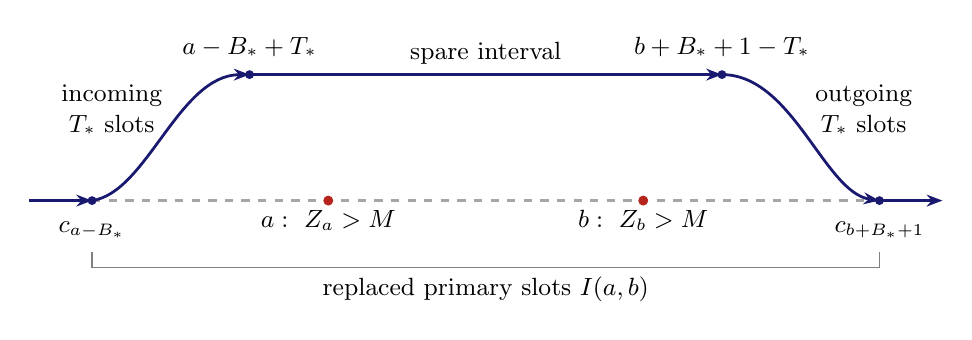
\begin{tikzpicture}[x=1cm,y=1cm,font=\small,
  route/.style={draw=MidnightBlue,line width=1pt,
    -{Stealth[length=2mm]}}]
 \draw[black!35,dashed,line width=0.8pt] (0,0)--(10,0);
 \draw[route] (-0.8,0)--(0,0);
 \draw[route] (10,0)--(10.8,0);
 \draw[route] (0,0) .. controls (0.7,0.1) and (1.1,1.6) .. (2,1.6);
 \draw[route] (2,1.6)--(8,1.6);
 \draw[route] (8,1.6) .. controls (8.9,1.6) and (9.3,0.1) .. (10,0);
 \fill[MidnightBlue] (0,0) circle (1.6pt) (2,1.6) circle (1.6pt)
   (8,1.6) circle (1.6pt) (10,0) circle (1.6pt);
 \fill[BrickRed] (3,0) circle (1.8pt) (7,0) circle (1.8pt);
 \node[below] at (3,0) {$a:\ Z_a>M$};
 \node[below] at (7,0) {$b:\ Z_b>M$};
 \node[above] at (2,1.7) {$a-B_*+T_*$};
 \node[above] at (8,1.7) {$b+B_*+1-T_*$};
 \node[above] at (5,1.6) {spare interval};
 \node[align=center] at (0.25,1.15) {incoming\\$T_*$ slots};
 \node[align=center] at (9.8,1.15) {outgoing\\$T_*$ slots};
 \node[below] at (0,-0.15) {$c_{a-B_*}$};
 \node[below] at (10,-0.15) {$c_{b+B_*+1}$};
 \draw[black!50] (0,-0.65)--(0,-0.85)--(10,-0.85)--(10,-0.65);
 \node[below] at (5,-0.85) {replaced primary slots $I(a,b)$};
\end{tikzpicture}
\caption{An accepted replacement, shown in nominal-parameter
coordinates. The marked primary slots are the extreme flags $a,b$ of
the accepted cluster; they may coincide. The flags use the matched cap
$M$, while the arrows show the actual uncapped physical route. The
diagram is schematic and does not represent a sampled FPP path; each
transition and the intervening spare piece is traversed forward.}
\label{improvement:fig-replacement}
\end{figure}

The latter instruction has an exact finite implementation. A proposed
leftmost flag $a$ and rightmost flag $b\in[a,a+L_*]$ form a complete
short cluster if and only if they are flagged, all consecutive flag
gaps in $[a,b]$ are at most $G_*$, and there is no flag in
$[a-G_*,a-1]$ or $[b+1,b+G_*]$. These tests read only
$[a-G_*,a+L_*+G_*]$. They can never accept a portion of a longer or
infinite cluster. Let $O_i$ indicate replacement of slot $i$. A cluster
covering $i$ has
\[
 a\in[i-L_*-B_*,i+B_*],
\]
so $O_i$ is determined by flags within distance $13B_*$ of $i$ and
transition tests within distance $10B_*$ of $i$. It follows in particular
that
\begin{equation}
 O_i\leq\sum_{a=i-L_*-B_*}^{i+B_*}F_a,
 \qquad \mathbb EO_i\leq H_*p.
 \label{improvement:flags:eq4}
\end{equation}

\emph{Uncovered positive costs.}
If a flagged slot is left uncovered because
its cluster is long or infinite, it contains a flag at distance
strictly greater than $R$. Following its chain from $i$ until the first
such flag gives an index $j$ with
\[
 R<|j-i|\leq R+G_*.
\]
There are $2G_*$ possible witnesses. If the cluster is short but not
accepted, one of the possible incoming tests indexed in
$[i-L_*-B_*,i-B_*]$, or outgoing tests indexed in
$[i+B_*,i+L_*+B_*]$, fails. Each of these at most $2(L_*+1)$ tests is
independent of $Z_i$, because its index is more than $R$ away. Applying
independence to these deterministic possible witnesses, before any
random choice of an extreme, gives
\begin{equation}
 \mathbb E[Z_i^+F_i(1-O_i)]
 \leq C_0\{2G_*p+2(L_*+1)\delta\}.
 \label{improvement:flags:eq5}
\end{equation}
For example each remote-flag term is
$\mathbb E[Z_i^+F_iF_j]=\mathbb E[Z_i^+F_i]p\leq C_0p$;
the failed-test terms are analogous. Thus the expectation of an
uncovered large cost is bounded directly, even if rare values carry a
substantial part of the first moment.

\emph{Retained and discarded primary costs.}
The retained costs satisfy
\begin{equation}
 (1-O_i)Z_i\leq W_i+MO_i+Z_i^+F_i(1-O_i).
 \label{improvement:flags:eq6}
\end{equation}
Indeed on a covered slot the right side is at least $-M+M=0$;
on an uncovered slot only the portion of $Z_i$ above $M$ can increase
its clipped value. In particular discarding negative primary costs
loses at most $M$ times the covered density, whether or not those
costs are correlated with nearby flags.

\emph{Replacement costs.}
By \eqref{improvement:flags:eq4} and independence of the entire spare
and primary fields,
\begin{equation}
 \mathbb E[V_iO_i]\leq H_*C_Vp.
 \label{improvement:flags:eq7}
\end{equation}
We have bounded the success indicator by the event of a nearby primary
flag; success itself need not be independent of $V_i$.

Accepted clusters have density at most $p$, so their two successful
transitions contribute at most $2K_\delta p$ to the mean upper bound.
Charge the remaining bound in \eqref{improvement:flags:eq3} to the
leftmost flag of its cluster. By stationarity, its mean per slot is
bounded by $\mathbb E[V_0O_0]$; unused spare slots in that display are
simply overcharged. Summing these bounds with
\eqref{improvement:flags:eq5}--\eqref{improvement:flags:eq7} proves
\eqref{improvement:flags:eq8}. Each charge and each reassignment involves
a uniformly bounded number of slots. Hence all charges are integrable,
and the expectation calculation requires only first moments.
\end{proof}

\subsection{Physical parameterization and endpoint accounting}
\label{improvement:locality}

The replacement lemma bounds stationary charges assigned to whole
pieces. Three further facts are needed to obtain an admissible road:
the physical concatenation must track the nominal line, its actual
period cuts must have the same mean excess as these charges, and its
full input support must remain bounded. We verify them in this order.

\paragraph{Tracking.}
Each crossing has horizontal drawdown at most $s/20$. The wall and
baseline attachments add only $O(r)$ to this drawdown; successive
walls have horizontal separation $a_0$. On each unchanged primary
slot, or each transition, take the running maximum of the horizontal
coordinate and apply the affine adjustment sending its endpoint
values to the prescribed endpoint parameters. This is continuous and
nondecreasing; constant portions are allowed. The adjustment moves
the horizontal nominal position by $O(s)$, since the horizontal
endpoint errors and the drawdown are $O(s)$. On spare portions use
the original spare nominal parameter. These parameterizations agree
at every concatenation and cover the real line.

Throughout a primary slot the vertical displacement from the nominal
line is $O(s)$. Throughout a transition it lies between its two baseline
offsets, up to $O(s)$, by
\eqref{improvement:transitions:eq1}--\eqref{improvement:transitions:eq2}.
Spare pieces have offset $10s$. Thus in the $(v,w)$ tracking norm the
entire output has tracking error at most $C_{\rm tr}s$, with
$C_{\rm tr}$ independent of the cluster and probability parameters.
Local edge repetitions and nominal pauses retain their occurrence
labels; no negative signed traversal is ever substituted for physical
motion.
Every baseline--wall and wall--link splice is at a lattice vertex.
A marked spare cut inside an edge only subdivides consecutive forward
travel along that same baseline occurrence. Merging those subdivisions
therefore leaves a two-sided lattice walk with locally finite edge
occurrences, as required by Definition~\ref{def:fb-road}.

\paragraph{Actual period cuts and integrability.}
To convert the charge bound \eqref{improvement:flags:eq8} into a mean
actual excess, assign the primary gauges to the designated primary
concatenation endpoints, and the compatible spare gauges to spare
endpoints. On each primary or transition piece interpolate its two
endpoint gauges linearly in the fraction of its positive physical
cost already traversed; on spare pieces use the spare interpolation.
These assignments agree at concatenations, are local, and commute
with translation by $A$. In particular they assign a gauge at every
actual first occurrence of an integer nominal level, including when
that occurrence precedes the designated endpoint during a nominal
pause. The assigned gauges are integrable at all these cuts.
Integrability on a transition follows from its positive physical
costs. On success, the total physical passage cost is at most
\[
 K_\delta\beta+|g_{\rm first}|+|g_{\rm last}|+C n,
\]
where the appropriate endpoint gauge may be $H_s$. The right side is
integrable by (G), and any physical subpiece costs at most the whole
physical path. A selected primary candidate has physical cost no
larger than its baseline competitor: their endpoints and corrections
are identical. That competitor lies in a fixed number of integrable
input periods. On primary and transition pieces, linear interpolation
bounds each assigned gauge by the absolute endpoint gauges. On spare
pieces, the original interpolation and (G) give integrability over
bounded parameter windows. Partial primary pieces, successful
transitions, and spare periods are therefore integrable.
This integrability is required at each fixed $n$; the bound need not be
uniform in $n$.

For an interval of $N$ slots, summing the local upper charges used in
\eqref{improvement:flags:eq8} bounds the corrected cost of all complete
primary and replacement pieces. Passing to the actual first-occurrence
endpoint cuts changes this bound only within the bounded number of
primary pieces and replacement intervals meeting the two boundaries.
The primary boundary pieces must be included even when no replacement
is accepted: a terminal wall arm may follow the first occurrence of
the terminal integer. Each boundary remainder is bounded by a fixed
finite sum of the integrable costs and gauges just described. Its
expected absolute value is bounded independently of $N$.
After division by $N$ this boundary error vanishes. The endpoint gauge
difference has zero mean: the complete output rule, including the
choice of endpoint label, is stationary under $A$, so the gauges at
translated cuts have the same integrable distribution. Thus
\eqref{improvement:flags:eq8} indeed bounds the expected actual $Q_n$
per old slot, divided by $\beta$. This uses stationarity of the chosen
labels and does not assume that the mean of the calibration at an
arbitrary random point is zero.

\paragraph{Input locality.}
The finite cluster test and the input supports in
Section~\ref{improvement:worlds} imply a fixed output dependence
radius $R_{\rm out}$ in old spatial units. Numerical caps affect only
comparisons of already calculated local quantities. The large
auxiliary boxes used to prove (L), and the size of its finite cap set,
are not inputs to this path construction. Neither $R_{\rm out}$ nor
$C_{\rm tr}$ depends on $s$, the directional tolerances, the cap, the
seam failure probability, or the input road rule.

\subsection{Choice of constants and contraction of the infimum}
\label{improvement:contraction}

The construction can now be closed in the class used to define $b(n)$.
The order of choices is essential: choose the rescaling from structural
support and tracking bounds first, then the small inward tilt, and only
then the probability and cap tolerances.

\begin{proposition}[Contraction in the original road class]
\label{improvement:contraction-proposition}
For suitable fixed rational $v,w$ near the flat endpoints and $s>0$,
there are an integer $D\ge1$ and $\rho<1$ such that
\[
 b(Dn)\le\rho b(n)
\]
for every sufficiently large admissible $n$. The infimum on both sides
uses the road class of Definition~\ref{def:fb-road}, with costs in their
original units.
\end{proposition}

\begin{proof}
The structural constants $C_{\rm tr},R_{\rm out},C_1$ are uniform
in sufficiently small $s$ and the nearby rational directions.
First choose an integer
\begin{equation}
 D\geq\max\{1000C_{\rm tr},R_{\rm out}/10,1\}.
 \label{improvement:contraction:eq2}
\end{equation}
Next fix rational $0<s<1/10$ and $\epsilon>0$ so small that
$DC_1s<1/4$ and $D\epsilon<1/4$. The geometry and the constants
$R,B_*,G_*,L_*,H_*,C_0,C_V$ have already been fixed uniformly.
If $C_0=0$, the primary costs vanish almost surely and no replacements
are necessary. Otherwise choose
\[
 \delta\leq\min\left\{\frac12,
       \frac{\epsilon}{6(L_*+1)C_0}\right\},
\]
then the corresponding transition cap $K_\delta$. Set
\[
 A_*=2G_*C_0+H_*C_V+2K_\delta,
 \qquad
 M_0\geq\max\{1,3C_0A_*/\epsilon\},
 \qquad \eta\leq\frac{\epsilon}{3(H_*+1)}.
\]
Choose the finite matched-cap range from (L) with this $M_0,\eta$,
and then fix the geometric comparison tolerances and the rational
directions so that it applies uniformly over that range. At every
sufficiently large admissible $n$, choose its deterministic good cap.
Equation~\eqref{improvement:primary:eq4} gives $Mp\leq\eta$, while
$p\leq C_0/M_0$ by Markov's inequality. In
\eqref{improvement:flags:eq8} the failed-test error, the terms
$A_*p$, and the terms $(H_*+1)\eta$ are each at most
$\epsilon/3$. We obtain an actual stationary local road with
\begin{equation}
 \mathbb E Q_n(\hbox{one old output slot})
       \leq(C_1s+\epsilon)\beta.
 \label{improvement:contraction:eq1}
\end{equation}
Regard $D$ old slots as one new period and use space units $Dn$.
The tracking error is then at most $s/1000$, the input radius at most
$10$, and the rule commutes with translation by $DA$ in old units,
that is by $A$ in new units. Reindexing the private product field by
this rescaling preserves its shift-invariant law: a new lattice shift
corresponds to the old lattice shift multiplied by $D$. Thus it is in the original road class at
scale $Dn$. The same construction in the other direction gives a pair
with common mean bound
\begin{equation}
 D(C_1s+\epsilon)\beta.
 \label{improvement:contraction:eq3}
\end{equation}
All the rational meshes have fixed denominators; multiplication of
an admissible $n$ by the integer $D$ preserves admissibility.

Let $b(n)$ be the infimum of the common mean bound over that road
class. Invoke the uniform input estimates with the fixed enlarged
prefactor $2C_s$; this changes only the threshold for $n$. That
threshold is therefore uniform over members with
$\beta\leq2C_s n^{1-c}$. Since $b(n)\leq C_s n^{1-c}$, for each
sufficiently small $t>0$ one can choose a pair with
$\beta\leq b(n)+t\leq2C_s n^{1-c}$. Apply
\eqref{improvement:contraction:eq3} and then let $t\downarrow0$; existence
of a minimizing road is unnecessary. This proves
\begin{equation}
 b(Dn)\leq D(C_1s+\epsilon)b(n).
 \label{improvement:contraction:eq4}
\end{equation}
All directions, meshes, and tolerances are fixed in the stated order,
and the choices give $\rho=D(C_1s+\epsilon)<1/2$. This proves the
assertion for all admissible $n$ above the common threshold.
\end{proof}

\section{Excluding flat faces}
\label{conclusion:section}

\begin{proof}[Proof of Theorem~\ref{thm:exponential-shape}]
Suppose $\partial\Bcal$ contains a nontrivial segment, and fix the
maximal supporting face with extreme endpoints $a,b$ described in
Section~\ref{model:section}. The same admissible road class has the
bounds
\[
 0<c_0\le b(n)\le C_s n^{3/4}
\]
from Propositions~\ref{prop:fb-positive} and \ref{prop:fb-upper}.

Proposition~\ref{improvement:contraction-proposition} supplies fixed
rational directions, $s>0$, an integer $D\ge1$, and $\rho<1$ such that
$b(Dn)\le\rho b(n)$ for every sufficiently large admissible $n$.
Choose an admissible $n_0$ above the common threshold. Multiplication
by $D$ preserves admissibility, so iteration gives
\[
 0<c_0\le b(D^k n_0)\le\rho^k b(n_0)
 \qquad(k\ge0),
\]
a contradiction. Thus every supporting face is a single point.

To express this as strict convexity, take distinct
$x,y\in\partial\Bcal$ and $0<t<1$. Convexity gives
$\mu((1-t)x+ty)\le1$. Equality would provide a supporting functional
$\ell\le\mu$ at this point, and therefore
\[
 1=(1-t)\ell(x)+t\ell(y),\qquad \ell(x),\ell(y)\le1.
\]
Both endpoint values would be one, so the entire segment $[x,y]$
would lie in a nontrivial supporting face. This has been excluded.
Therefore $\mu((1-t)x+ty)<1$ for the rate-one exponential law.

Theorem~\ref{thm:gamma-differentiability} with shape $\kappa=1$
gives Fr\'echet differentiability of this norm away from the origin and
a $C^1$ unit sphere, with a unique supporting line at every point.
To pass to any rate $\lambda>0$, couple the weights by
$\tau_e^{(\lambda)}=\lambda^{-1}\tau_e^{(1)}$. Then every path cost,
and hence every passage time, is multiplied by $\lambda^{-1}$. Thus
\[
 T_\lambda(x,y)=\lambda^{-1}T_1(x,y),\qquad
 \mu_\lambda=\lambda^{-1}\mu_1,\qquad
 \Bcal_\lambda=\lambda\Bcal_1.
\]
Multiplication by a positive scalar preserves differentiability,
strict convexity, and the $C^1$ boundary property. This proves every
assertion of the theorem.
\end{proof}

\section{Geometric and geodesic consequences}
\label{sec:consequences}

The first two subsections concern the exponential law of arbitrary rate
$\lambda>0$. Theorem~\ref{thm:exponential-shape} supplies both regularity
properties needed there. The final two subsections apply
Theorem~\ref{thm:gamma-differentiability} to a quantitative midpoint
estimate and to cone-tip competition for the whole Gamma family.

For a Euclidean unit vector $u$, put $v_u=u/\mu(u)$ and
$\rho_u=\nabla\mu(u)$. Homogeneity gives
$\rho_u\cdot v_u=1$, and the supporting inequality gives
$\rho_u\cdot x\le\mu(x)$ for every $x$. Hence
\[
 P_u=\{x:\rho_u\cdot x=1\}
\]
is the supporting line at $v_u$. Strict convexity gives
$P_u\cap\Bcal=\{v_u\}$: two contact points would put their entire
segment in the boundary. Thus the set of radial directions of contact
with $P_u$ consists of the single direction $u$.

\subsection{A fixed deterministic direction}

A finite geodesic is a path realizing the passage time between its
endpoints. An infinite geodesic, or a bigeodesic, is respectively a
one-sided or two-sided infinite path every finite segment of which is
a finite geodesic. For the Gamma laws in this paper, finite geodesics
exist and are almost surely unique. Indeed, choose $\theta>0$ so large
that $3\E e^{-\theta\tau_e}<1$. Counting simple paths shows that the
probability of a simple path from a fixed vertex with at least $m$
edges and cost at most $t$ is bounded by
$C e^{\theta t}(3\E e^{-\theta\tau_e})^m$. Thus almost surely only
finitely many simple paths from that vertex have cost below any fixed
bound. Thus every passage ball $\{z:T(x,z)\le t\}$ is finite, and a
minimum is attained between any two vertices. Two distinct simple paths with the
same endpoints have different edge sets; conditioning on all but an
edge in their symmetric difference shows that their costs are unequal
almost surely. Countability gives uniqueness simultaneously for all
lattice endpoints.

A sequence $(z_n)$ is directed toward a unit vector $u$ when
$\lVert z_n\rVert_2\to\infty$ and
$z_n/\lVert z_n\rVert_2\to u$. An infinite geodesic has direction $u$
when its vertex sequence has this property. Write $\Gamma(x,y)$ for the
unique finite geodesic between lattice vertices $x$ and $y$. Local
convergence of paths rooted at $x$ means eventual agreement of each fixed
finite initial segment.

\begin{corollary}\label{cor:fixed-direction}
Fix a deterministic unit vector $u$. There is an event $\Omega_u$ of
probability one on which all the following statements hold.
\begin{enumerate}
\item For every $x\in\Z^2$ there is exactly one infinite geodesic
      $\Gamma_x^u$ from $x$ with direction $u$. For every sequence $(z_n)$
      directed toward $u$, including a sequence chosen from the edge
      configuration,
      $\Gamma(x,z_n)\to\Gamma_x^u$ locally.
\item For every $x,y\in\Z^2$, the paths $\Gamma_x^u$ and
      $\Gamma_y^u$ have a common tail.
\item No bigeodesic has an end with direction $u$.
\item For every $x,y\in\Z^2$, the limit
\[
 B_u(x,y)=\lim_{n\to\infty}\bigl(T(x,z_n)-T(y,z_n)\bigr)
\]
      exists and is independent of the choice of sequence directed toward
      $u$. Moreover,
\[
 \E B_u(0,x)=\nabla\mu(u)\cdot x,
\]
      and, for every $\varepsilon>0$, only finitely many $x\in\Z^2$
      satisfy
\[
 |B_u(0,x)-\nabla\mu(u)\cdot x|>\varepsilon\lVert x\rVert_1.
\]
\end{enumerate}
\end{corollary}

\begin{proof}
Damron--Hanson's product-measure hypothesis A1$'$ holds: the common law
is continuous, and the minimum $Y$ of the four weights incident to the
origin is exponential of rate $4\lambda$, whence
$\E Y^2=1/(8\lambda^2)<\infty$.
Their geometric assumptions (2.1)--(2.2) require differentiability at
the chosen boundary point and at both endpoints of its supporting face.
The preceding supporting-line calculation identifies that face with
$\{v_u\}$. Thus their supporting sector is exactly the direction $u$.
Theorems~1 and~2 of \cite{DH2017} give the convergence, coalescence,
bigeodesic exclusion, and Busemann statements on one probability-one
event for this fixed $u$. Their normalized supporting vector is
$\rho_u=\nabla\mu(u)$ by that calculation.

For completeness, uniqueness follows from the convergence assertion.
If $(x=x_0,x_1,\ldots)$ is any infinite geodesic of direction $u$, then
its segment ending at $x_n$ is $\Gamma(x,x_n)$ by uniqueness of finite
geodesics. These segments converge both to that infinite geodesic and
to $\Gamma_x^u$, so the paths agree.
\end{proof}

The Busemann limit also has an elementary pathwise description. If $c$
is any common vertex after $\Gamma_x^u$ and $\Gamma_y^u$ have coalesced,
local convergence implies that both finite geodesics to $z_n$ pass
through $c$ for all sufficiently large $n$. Hence
\begin{equation}\label{eq:busemann-common-vertex}
 B_u(x,y)=T(x,c)-T(y,c).
\end{equation}
In particular the displayed difference defining $B_u(x,y)$ is eventually
constant for each fixed pair and each such target sequence. Taking limits
in the triangle inequality and in differences of passage times gives
\[
 |B_u(x,y)|\leq T(x,y),\qquad
 B_u(x,z)=B_u(x,y)+B_u(y,z).
\]
The first inequality also gives integrability. If $y$ lies on
$\Gamma_x^u$, then $B_u(x,y)=T(x,y)$. Translation of the environment and
of the targets shows that this additive random function is stationary.

The direction $u$ is fixed before taking the probability-one event.
One may intersect these events for a prescribed countable set of
directions. The result does not assert simultaneous uniqueness in all
directions, or simultaneous absence of all bigeodesics.

Independently of these shape arguments, the companion manuscript
\cite[Theorem~1.1]{OpenAINoBigeodesics2026} excludes all bigeodesics on one
probability-one event for iid $\operatorname{Gamma}(\kappa,\lambda)$ edge
weights, for each fixed $\kappa,\lambda>0$. This includes the exponential
laws here; these distributions satisfy its nonatomic minimum-second-moment
hypotheses.

\subsection{Passage through a prescribed vertex}

\begin{corollary}\label{cor:midpoint}
For every nonzero $v\in\Z^2$,
\[
 \lim_{n\to\infty}
 \PP\bigl(\lfloor n/2\rfloor v\in\Gamma(0,nv)\bigr)=0.
\]
More generally, let $a_n,b_n,z_n$ be deterministic lattice vertices with
\[
 \lVert a_n-z_n\rVert_2\to\infty,
 \quad\lVert b_n-z_n\rVert_2\to\infty,
 \quad
 \frac{b_n-z_n}{\lVert b_n-z_n\rVert_2}\longrightarrow u
\]
for a deterministic unit vector $u$. Then
$\PP(z_n\in\Gamma(a_n,b_n))\to0$.
\end{corollary}

\begin{proof}
Set $p_n=a_n-z_n$ and $q_n=b_n-z_n$. Translation invariance gives
$\PP(z_n\in\Gamma(a_n,b_n))=
\PP(0\in\Gamma(p_n,q_n))$.
If the asserted probabilities had positive limsup,
the event that $0\in\Gamma(p_n,q_n)$ for infinitely many $n$ would
have positive probability. Intersect this event with $\Omega_u$ from
Corollary~\ref{cor:fixed-direction}.
Restrict to the infinite set of indices for which
$0\in\Gamma(p_n,q_n)$. On the intersection, the arm from $0$ to $q_n$ converges locally to
$\Gamma_0^u$. Both arms have lengths tending to infinity, since their
endpoints tend to infinity. Local finiteness of the lattice permits a
diagonal subsequence along which the other arm also converges to an
infinite path. Every finite segment of the resulting two-sided path is
a segment of one of the finite geodesics $\Gamma(p_n,q_n)$, and hence
is geodesic. The two arms have no vertex in common except $0$, because
each finite geodesic is simple. This constructs a bigeodesic with an
end of direction $u$, contradicting Corollary~\ref{cor:fixed-direction}.
The first assertion uses $a_n=0$, $b_n=nv$, and
$z_n=\lfloor n/2\rfloor v$.
\end{proof}

This is the compactness argument underlying \cite[Theorem~2.1]{DH2017}.
Ahlberg and Hoffman \cite[Theorem~2.1]{AH2019} already prove the whole
qualitative corollary for arbitrary deterministic endpoint sequences
escaping from the tested site, assuming continuity and the
minimum-of-four second moment. This includes all Gamma laws here and
requires no shape regularity. The proof above records its connection
with the fixed-direction consequences.

\subsection{A quantitative midpoint bound for Gamma weights}

Differentiability has a useful consequence even when strict convexity
has not been established: a $C^1$ planar convex body cannot have only
finitely many extreme points. This verifies the geometric hypothesis
of the quantitative midpoint theorem of Dembin, Elboim, and Peled.

\begin{corollary}[Quantitative midpoint bound for the Gamma family]
\label{cor:gamma-quantitative-midpoint}
For every $\kappa>0$ there is $C_\kappa<\infty$ such that, for every
$\lambda>0$ and all $a,b,z\in\Z^2$ with
$D=\min\{\lVert a-z\rVert_1,\lVert b-z\rVert_1\}\geq1$,
\[
 \PP\bigl(z\in\Gamma_{\kappa,\lambda}(a,b)\bigr)
 \leq C_\kappa\frac{\log^2(D+2)}{D^{1/16}},
\]
where $\Gamma_{\kappa,\lambda}$ denotes the unique geodesic for
iid $\operatorname{Gamma}(\kappa,\lambda)$ edge weights.
\end{corollary}

\begin{proof}
Theorem~\ref{thm:gamma-differentiability} gives a $C^1$ boundary. We verify that such a
compact planar convex body has infinitely many extreme points.
At a boundary point choose a supporting line. Its intersection with
the body is a point or a compact segment, and its endpoints are
extreme points of the body: any convex decomposition of an endpoint
must stay in the supporting line, where extremality is immediate.
Thus every boundary point is a convex combination of extreme points.
Every interior point lies between two boundary points, so the whole
body is the convex hull of its extreme points. If there were only
finitely many, the body would be a polygon with nonempty interior.
At a vertex of that polygon the two adjacent sides give distinct
supporting lines, contradicting differentiability. Hence the number
of extreme points exceeds forty.

The Gamma density is absolutely continuous, has no atom at zero,
and has a finite exponential moment by Lemma~\ref{df:ga:moment}.
All the hypotheses of \cite[Theorem~1.2]{DEP2024} are therefore
satisfied. Apply that theorem at rate one to obtain $C_\kappa$.
The coupling $t_e^{(\kappa,\lambda)}=
t_e^{(\kappa,1)}/\lambda$ leaves every geodesic unchanged and proves
the assertion for all positive rates with the same constant.
\end{proof}

For Gamma laws, differentiability also verifies the tangent and
supporting-face endpoint assumptions of \cite{DH2017}. Its conclusions
then retain the supporting-sector formulation. The single-direction
statements of Corollary~\ref{cor:fixed-direction} use the strict
convexity established for exponential weights.

\subsection{Cone-tip competition for Gamma weights}

We apply the tangent theorem of Ahlberg, Deijfen, and Sfragara
\cite[Theorem~1]{ADS2026} to their simultaneous cone-versus-tip initial
configuration.

\begin{corollary}[Gamma and Richardson cone-tip survival]
\label{cor:gamma-cone-tip}
Fix $\kappa,\lambda>0$, a deterministic unit vector $\theta\in S^1$,
and a geometric half-angle $0\le\alpha\le\pi$. Define the closed cone
\[
 \begin{aligned}
 C^\theta_\alpha&=\{0\}\cup
 \{x\in\R^2\setminus\{0\}:\angle(x,-\theta)\le\alpha\},\\
 I_1&=(C^\theta_\alpha\cap\Z^2)\setminus\{0\},
 \qquad I_2=\{0\},
 \end{aligned}
\]
where $\angle(x,-\theta)$ is the Euclidean angle between the two vectors.
Use one iid $\operatorname{Gamma}(\kappa,\lambda)$ field on unoriented
nearest-neighbor edges of $\Z^2$, with passage metric $T$. At time zero,
start type 1 from every site of $I_1$ and type 2 from $I_2$.
Both types use this same realization of $T$, and each site is permanently
claimed by the type that reaches it first. With
$T(I,z)=\inf_{x\in I}T(x,z)$, interpreting the infimum of the empty set
as $\infty$, the sites eventually claimed by type 2 are almost surely
\[
 \mathcal E_2=\{z\in\Z^2:T(0,z)<T(I_1,z)\}.
\]
Then
\[
 \PP\bigl(|\mathcal E_2|=\infty\bigr)>0
 \quad\Longleftrightarrow\quad
 \alpha<\pi/2.
\]
In particular, at $\alpha=\pi/2$, when the cone is the closed half-plane
$\{x:x\cdot\theta\le0\}$, type 2 claims only finitely many sites almost
surely. At $\kappa=1$, this gives Benjamini's cone-tip prediction for
equal-rate Richardson competition with any common rate $\lambda>0$ in
the same initial configuration.
\end{corollary}

\begin{proof}
The Gamma law is atomless for every $\kappa>0$, including $\kappa<1$.
For four independent samples,
\[
 \E\bigl[\min(\tau_1,\ldots,\tau_4)^2\bigr]
 \le \E\tau_1^2
 =\frac{\kappa(\kappa+1)}{\lambda^2}<\infty.
\]
Thus the continuity and minimum-second-moment hypotheses of
\cite[Theorem~1]{ADS2026} hold.

The infinite seed set causes no ambiguity in the arrival-time comparison.
If $I_1$ is nonempty, choose one seed as a finite upper bound for
$T(I_1,z)$. Only finitely many seeds lie in the corresponding passage
ball about $z$, so the infimum is attained. Simple paths from distinct
seeds to $z$ have different edge sets. Conditioning on all edge weights
except one in their symmetric difference and using atomlessness rules
out equal costs;
countability gives this simultaneously for all such paths and sites.
Thus the shared-metric competition is described by the displayed strict
comparison defining $\mathcal E_2$.

Theorem~\ref{thm:gamma-differentiability} gives a $C^1$ boundary.
For the fixed $\theta$, put
$h(\theta)=\max_{x\in\Bcal}x\cdot\theta>0$. The supporting line
\[
 L_\theta=\{x:x\cdot\theta=h(\theta)\}
\]
is perpendicular to the positive $\theta$-ray and meets that ray at
$h(\theta)\theta$. At any contact point with $\Bcal$, the $C^1$ boundary
makes $L_\theta$ the unique supporting line, hence a tangent in the
sense of \cite{ADS2026}; the contact point need not lie on the ray.
For a seed set $I\subset\Z^2\setminus\{0\}$, write
$\mathcal E_2(I)=\{z\in\Z^2:T(0,z)<T(I,z)\}$, with the same
empty-set convention for $T(I,z)$. If $I\subset J$, then
$T(J,z)\le T(I,z)$ and hence
$\mathcal E_2(J)\subset\mathcal E_2(I)$. If $\alpha<\pi/2$, choose
$\alpha<\alpha'<\pi/2$. The source's cone of half-angle $\alpha'$
contains the closed $\alpha$-cone, regardless of its boundary convention,
so its Theorem~1 gives positive survival for the closed $\alpha$-cone
as well. If
$\alpha\ge\pi/2$, the closed $\alpha$-cone contains the closed critical
half-plane. Theorem~5 gives almost-sure finite type-2 growth for that
half-plane, and monotonicity gives the same conclusion for the larger
cone. This proves the stated closed-cone convention throughout
$[0,\pi]$, without strict convexity, for every prescribed orientation.

When $\kappa=1$, the shared exponential edge field gives the equal-rate
two-type Richardson model. The coupling
$\tau_e^{(\lambda)}=\tau_e^{(1)}/\lambda$ multiplies both arrival
times by the same positive constant and leaves every comparison
defining $\mathcal E_2$ unchanged. This proves the stated specialization.
\end{proof}

The probability assertion is for each fixed orientation, not a simultaneous
pathwise statement over all directions. Below the threshold it asserts a
positive survival probability without claiming that this probability is one.
It does not address unequal rates, independent type-specific metrics,
coexistence from two finite seed sets, or the rate or asymptotic shape of
type-2 growth.

\bibliographystyle{plain}
\bibliography{references}
\end{document}
